% !TeX program = XeLaTeX
\documentclass[9pt,svgnames]{extbook}
% \usepackage[b5paper, top=10mm, text={144mm, 208mm}, includehead, includefoot, hmarginratio=1:1, heightrounded]{geometry}
\usepackage[a4paper, top=16mm, text={170mm, 246mm}, includehead, includefoot, hmarginratio=1:1, heightrounded]{geometry}
	% \pdfpagewidth=176truemm
	% \pdfpageheight=250truemm
	\pdfpagewidth=210truemm
	\pdfpageheight=297truemm
\usepackage[explicit,clearempty]{titlesec}
\usepackage{wallpaper,changepage,fancyhdr,tikz,indentfirst}
\usepackage{amssymb,amsfonts,amsthm,bm,mathrsfs,etoolbox}
\usepackage[leqno]{amsmath}
% \def\pgfsysdriver{pgfsys-dvipdfm.def}
\usepackage[all]{xy}
\usetikzlibrary{shapes,positioning}
\usepackage{hyperref}
	\hypersetup{bookmarksnumbered=true}

%% Define how the chapter title is printed
\titleformat{\chapter}{}{}{0pt}{
%% Background image at top of page
%% Draw a semi-transparent rectangle across the top
	%% Check if on an odd or even page
	\strictpagecheck\checkoddpage
	\ifoddpage{
	}
	\else {
		\newpage
		\thispagestyle{plain}
	}
	\fi
	\tikz[overlay,remember picture]
	\fill[opacity=.7]
	(current page.north west) rectangle 
	([yshift=-3cm] current page.north east);
	\begin{tikzpicture}[overlay,remember picture]
	\node[anchor=south west,text=white,
		xshift=20mm,yshift=-25mm,
		font=\sffamily\bfseries\huge] 
		at (current page.north west) 
		{\chaptername\ \thechapter};
	\node[fill=Sienna!80!black,text=white,
		font=\Huge\bfseries, 
		inner ysep=12pt, inner xsep=20pt,
		rounded rectangle,anchor=east, 
		xshift=-20mm,yshift=-30mm] 
		at (current page.north east) {#1};
	\end{tikzpicture}
}
%% Define how the chapter title is printed
\titleformat{name=\chapter,numberless}{}{}{0pt}{
%% Draw a semi-transparent rectangle across the top
\tikz[overlay,remember picture]
	\fill[opacity=.7]
	(current page.north west) rectangle 
	([yshift=-3cm] current page.north east);
	\begin{tikzpicture}[overlay,remember picture]
	\node[fill=Sienna!80!black,text=white,
		font=\Huge\bfseries, 
		inner ysep=12pt, inner xsep=20pt,
		rounded rectangle,anchor=east, 
		xshift=-20mm,yshift=-30mm] 
		at (current page.north east) {#1};
	\end{tikzpicture}
}
\titlespacing*{\chapter}{0pt}{0pt}{120mm}
\titlespacing*{name=\chapter,numberless}{0pt}{0pt}{60mm}

%% Set the uniform width of the colour box
%% displaying the page number in footer
%% to the width of "99"
\newlength\pagenumwidth
\settowidth{\pagenumwidth}{99}

%% Define style of page number colour box
\tikzset{pagefooter/.style={
anchor=base,font=\sffamily\bfseries\small,
text centered,text depth=17mm,text width=\pagenumwidth}}

%% Concoct some colours of our own
\definecolor[named]{GreenTea}{HTML}{000000}

%%%%%%%%%%
%%% Re-define running headers on non-chapter pages
%%%%%%%%%%
\fancypagestyle{headings}{%
	\fancyhf{}   % Clear all headers and footers first
	%% Right headers on odd pages
	\fancyhead[RO]{%
	%% First draw the background rectangles
	%% Then the decorative line and the right mark
	\begin{tikzpicture}[xshift=-.75\baselineskip,yshift=.25\baselineskip,remember picture,    overlay,fill=GreenTea,draw=GreenTea]\fill circle(3pt);\draw[semithick](0,0) -- (current page.west |- 0,0);\end{tikzpicture} \sffamily\itshape\small\nouppercase{\rightmark}
	}

	%% Left headers on even pages
	\fancyhead[LE]{%
	%% Background rectangles first
	%% Then the right mark and the decorative line
	\sffamily\itshape\small\nouppercase{\leftmark}\ 
	\begin{tikzpicture}[xshift=.5\baselineskip,yshift=.25\baselineskip,remember picture, overlay,fill=GreenTea,draw=GreenTea]\fill (0,0) circle (3pt); \draw[semithick](0,0) -- (current page.east |- 0,0 );\end{tikzpicture}
	}

	%% Right footers on odd pages and left footers on even pages,
	%% display the page number in a colour box
	\fancyfoot[RO,LE]{\tikz[baseline]\node[pagefooter]{\thepage};}
	\renewcommand{\headrulewidth}{0pt}
	\renewcommand{\footrulewidth}{0pt}
}

%%%%%%%%%%
%%% Re-define running headers on chapter pages
%%%%%%%%%%
\fancypagestyle{plain}{%
	%% Clear all headers and footers
	\fancyhf{}
	%% Right footers on odd pages and left footers on even pages,
	%% display the page number in a colour box
	\fancyfoot[RO,LE]{\tikz[baseline]\node[pagefooter]{\thepage};}
	\renewcommand{\headrulewidth}{0pt}
	\renewcommand{\footrulewidth}{0pt}
}
% \usepackage[fontset=windows]{ctex}
\usepackage[fontset=fandol]{ctex}
	% \CTEXoptions[today=old]
	% \CTEXoptions[contentsname=Table of Contents]
\usepackage{paralist,wrapfig}
	\setlength{\pltopsep}{3pt}
	\setlength{\plpartopsep}{3pt}
\usepackage{titletoc,makeidx}
	\setcounter{secnumdepth}{5}  
	\setcounter{tocdepth}{5} 
	\makeindex

\renewcommand\thechapter{\Roman{chapter}}

\usepackage{hyperref}
	\hypersetup{bookmarksnumbered=true}

% \newcommand{\no}[1]{$(#1)$}
% \renewcommand{\not}[1]{#1\!\!\!/}
\newcommand{\rr}{\mathbb{R}}
\newcommand{\zz}{\mathbb{Z}}
\newcommand{\cc}{\mathbb{C}}
\newcommand{\aaa}{\mathfrak{a}}
\newcommand{\pp}{\mathfrak{p}}
\newcommand{\mm}{\mathfrak{m}}
\newcommand{\dd}{\mathrm{d}}
\newcommand{\oo}{\mathscr{O}}
\newcommand{\ff}{\mathscr{F}}
\newcommand{\scrg}{\mathscr{G}}
\newcommand{\scr}[1]{\mathscr{#1}}
\newcommand{\bbp}{\mathbb{P}}
\newcommand{\bba}{\mathbb{A}}
\def\A{\mathbb{A}}
\def\P{\mathbb{P}}

\DeclareMathOperator{\im}{im}
\DeclareMathOperator{\Hom}{Hom}
\DeclareMathOperator{\id}{id}
\DeclareMathOperator{\rank}{rank}
\DeclareMathOperator{\tr}{tr}
\DeclareMathOperator{\supp}{supp}
\DeclareMathOperator{\coker}{coker}
\DeclareMathOperator{\codim}{codim}
\DeclareMathOperator{\height}{height}
\DeclareMathOperator{\sign}{sign}
\DeclareMathOperator{\spec}{Spec}
\DeclareMathOperator{\proj}{Proj}
\DeclareMathOperator{\res}{res}

\DeclareMathOperator{\Gal}{Gal}
\DeclareMathOperator{\ann}{ann}
\DeclareMathOperator{\Ann}{Ann}
\DeclareMathOperator{\ev}{ev}

\newcommand{\hyp}{-}
\newcommand{\nottran}{\rule{2mm}{2mm}}
\newcommand{\idx}[1]{\textit{#1}\index{#1}}
\newcommand{\idxx}[2]{\textit{#2}\index{#1!#2}}

\newcommand{\moha}[1]{\stackon[1pt]{#1}{\hbox to 0pt{\hss
\includegraphics[width=.8em,bb=0 0 118 66]{naive.pdf}\hss}}}
\newcommand{\Naive}{Na\moha{\i}ve}
\newcommand{\naive}{na\moha{\i}ve}

\theoremstyle{plain}
\newtheorem{thm}{Theorem}[chapter]
\newtheorem{pro}[thm]{Proposition}
\newtheorem{lem}[thm]{Lemma}
\newtheorem{coro}[thm]{Corollary}

\theoremstyle{definition}
\newtheorem{defi}[thm]{Definition}
\newtheorem{exe}[thm]{Exercise}
\newtheorem{exa}[thm]{Example}

\renewcommand*{\proofname}{Proof}
\renewcommand{\thethm}{\thechapter\raisebox{.15ex}{-}\arabic{thm}}

\renewcommand\thechapter{\Roman{chapter}}
	\newcommand{\cc}{\mathbb{C}}

\newcommand{\picc}[1]{\begin{center}\includegraphics[scale=0.5]{#1}\end{center}}
\newcommand{\pic}[1]{\picc{#1}}

\begin{document}
\begin{titlepage}
\setcounter{page}{-1}
\thispagestyle{empty}
	\begin{flushright}
	{\Huge\bfseries 概形的几何}\\[\baselineskip]
	% {{\scshape In\:}\Large {\itshape a simple} {\scshape Way}} \par
	{by xxx}\par
	\today
	\end{flushright}
	\vfill
	{\Large\itshape 仅作内部交流用}
\end{titlepage}
\clearpage
\frontmatter
\pagestyle{plain}
\ThisULCornerWallPaper{1}{Pictures/0.png}
\tableofcontents
\mainmatter
\pagestyle{headings}
	\chapter*{前言}
暂略。
	\renewcommand{\pic}[1]{\picc{chap_1/pics/#1}}

\chapter{基本定义}
\ThisULCornerWallPaper{1}{Pictures/1.png}
	\renewcommand{\pic}[1]{\picc{chap_2/pics/#1}}

\chapter{例子}\label{chap:2}
\ThisULCornerWallPaper{1}{Pictures/2.png}
\section{代数闭域上的约态概形}

概形概念的发始,即是想要推广经典的代数闭域上的仿射簇,我们将从它开始一系列关于概形的例子。在这里,代数闭域$K$上的仿射簇是指一个仿射概形$\spec R$,其中$R$是一个簇$X$的坐标环\index{坐标环},即$R$是一个有限生成的约态$K$\hyp 代数\index{约态!代数}。(回忆一个环是约态的,是指它没有非零幂零元。)$\spec R$时常被叫做\textit{相伴于簇}$X$的概形\footnote{译者注:在下面的行文中,翻译中也会将$\spec R$称为$X$的相伴概形。同时,有时候也会反过来,称一个簇或者闭点相伴于某个概形。由于有时候一个理想也给出一个簇,所以有时也会用相伴于理想的概形,或者理想的相伴概形等说法。}:这种概形有时就直接被称作仿射簇。在以后几节中,我们将考虑不同于这个基本模型的概形。

相伴于代数闭域$K$上的仿射簇的$K$\hyp 概形与这个簇是等价的对象:它们都可以决定一个相同的坐标环或者被一个相同的坐标环决定。但是,在这个例子中已经有所表现的是,在概形理论中,一些经典的概念,比如簇的相交或者映射的纤维,应有更精确的解释。在这以及接下来的章节中,我们将看到这个现象的例子。

\subsection{仿射空间}

我们从概形$\mathbb{A}^n_K:=\spec K[x_1$, $\dots$, $x_n]$开始,其中$K$是一个代数闭域。这个概形被称为$K$上的\textit{仿射}$n$-\textit{空间}。

这里将使用一个标准但绝不平凡的代数结论 ------ Hilbert's Nullstellensatz(零点定理)的一种形式;比如可见 Eisenbud [1995].

\begin{thm}[Nullstellensatz]
	设$K$是一个域,如果$\mathfrak{m}$是多项式环$K[x_1$, $\dots$, $x_n]$的一个极大理想(或者更一般地,$p$是$K$上的一个代数空间的子簇的一个闭点),则
	\[
		K[x_1, \dots, x_n]/\mathfrak{m}=\kappa(p)
	\]
	是一个有限维$K$\hyp 矢量空间。
\end{thm}

在我们的例子中,$K$是代数闭的,这就意味着$\kappa(p)=K$. 因此,记$\lambda_i$是$x_i$在$\kappa(p)$中的像,可以看到
\[
	\mathfrak{m}=(x_1-\lambda_1, \dots, x_n-\lambda_n).
\]
于是,$\mathbb{A}^n_K$中的闭点与$K$中元素的$n$元组相对应,正如期望的那般。有时,我们会用“点$(\lambda_1$, $\dots$, $\lambda_n)$”来指代“点$[(x_1-\lambda_1$, $\dots$, $x_n-\lambda_n)]$”. 

从一维的情况开始,仿射直线
\[
	\mathbb{A}^1_K=\spec K[x]
\]
长得就像它的经典对应,同样被叫做仿射直线的仿射簇。在仿射直线上,每一个$\lambda\in K$都对应有一个闭点,闭点构成的集合上的Zariski拓扑也与仿射簇上的经典的Zariski拓扑相同:开集是有限集的补。概形$\mathbb{A}^1_K$与簇不同的地方只在于它多了一个点,这个点被称为\textit{一般点}\index{一般!点}%
\footnote{译者注:作者后面才会给出明确的定义,这里事先给一下:如果$Y=\overline{\{x\}}$,则称$x$是$Y$的一个一般点。一般而言,一般点可能不存在,也可能不唯一。}%
,对应于零理想$(0)$。
\vspace{-1ex}\begin{center}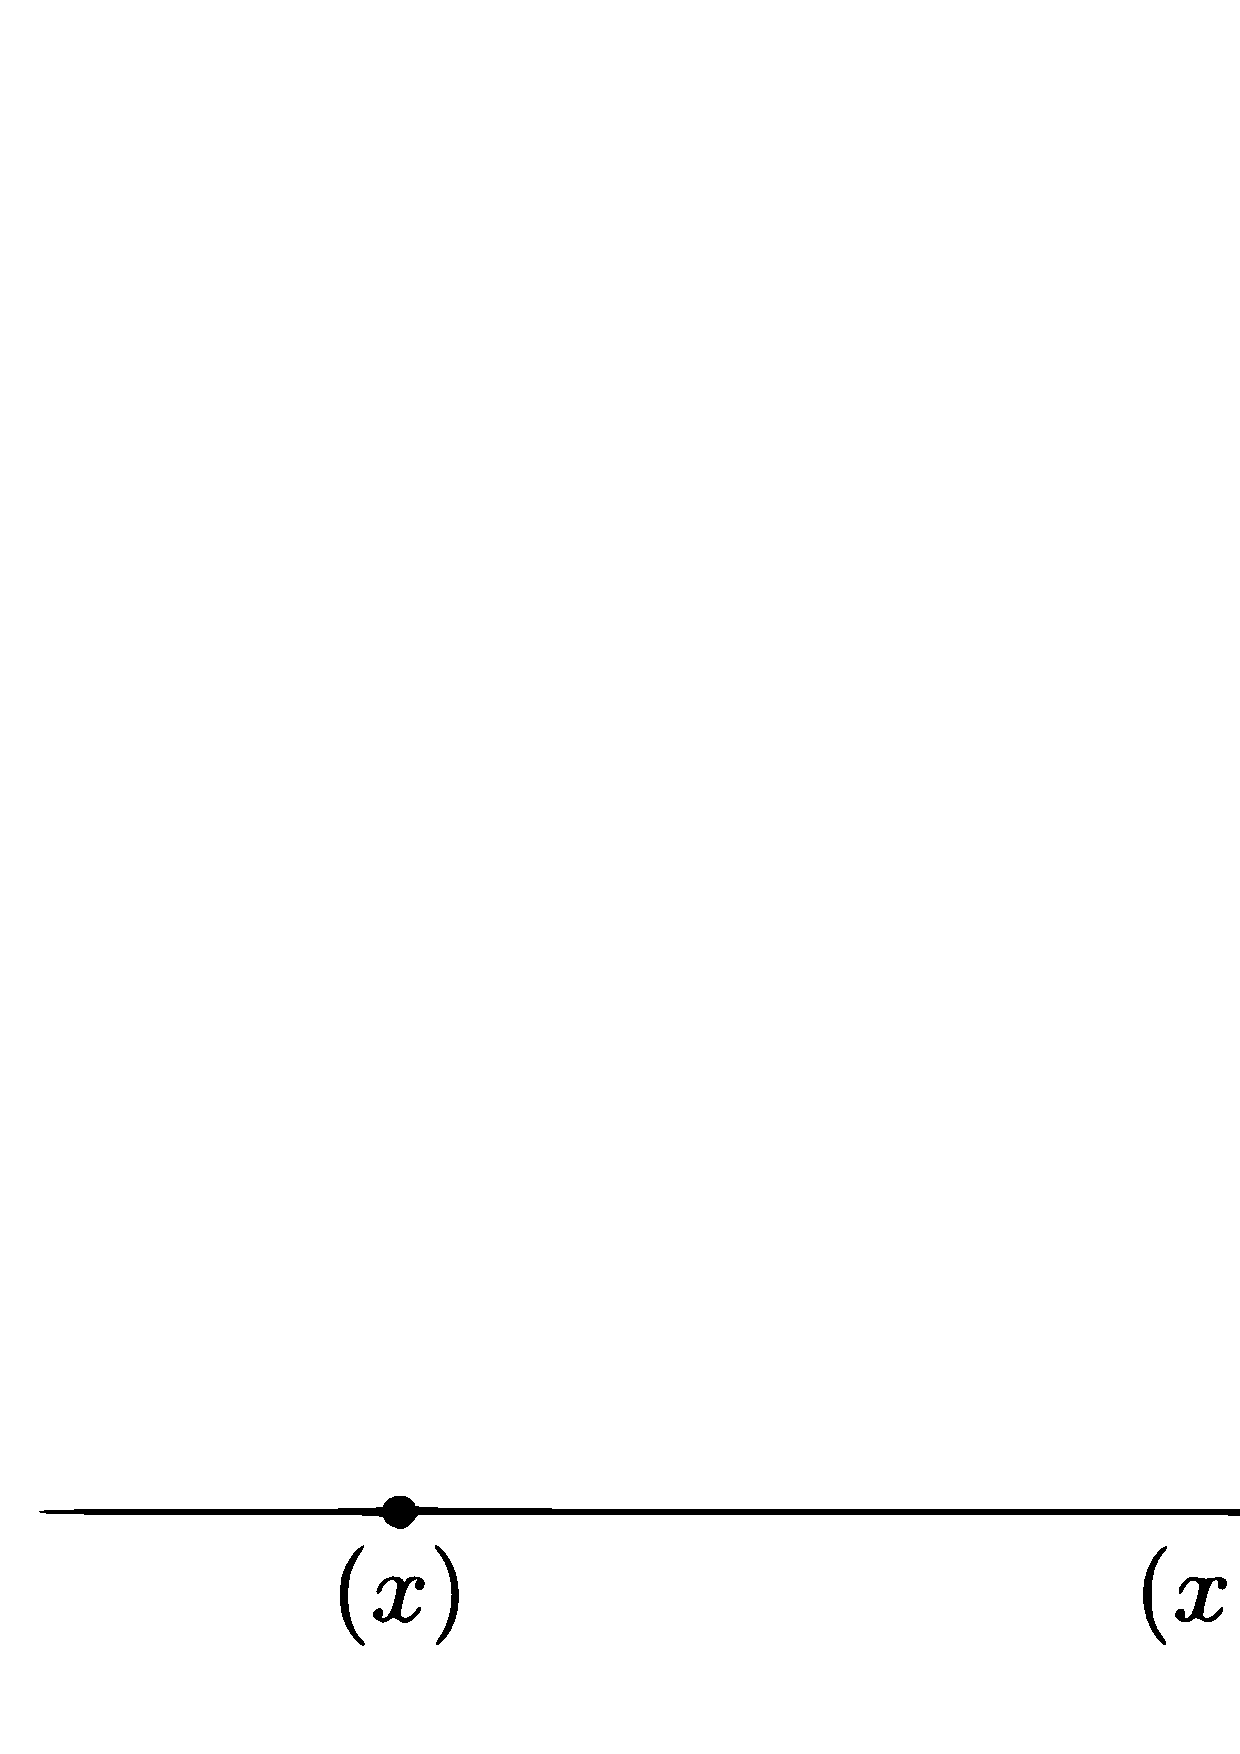
\includegraphics[scale=\scale,bb=0 0 447 81]{\PICDIR/1.png}\end{center}
\vspace{-2ex}点$(0)$的闭包是整个$\mathbb{A}^1_K$,因此,$\mathbb{A}^1_K$的闭子集就是$\mathbb{A}^1_K-\{(0)\}$的有限子集。

仿射平面$\mathbb{A}^2_K=\spec K[x,y]$同样与它的经典对应相似,但现在就多了许多点,同时也表现得更加有趣。像之前一样,我们有来自于极大理想$(x-\lambda,y-\mu)$的闭点,对应于寻常平面中的$(\lambda,\mu)$. 但现在却有两类非闭点。首先,对每一个不可约多项式$f(x,y)\in K[x,y]$,有一点$p$对应于素理想$(f)\subset K[x,y]$,它的闭包包含$p$本身以及所有使得$f(\lambda,\mu)=0$的闭点$(\lambda,\mu)$,点$(f)$被称为该集合的一般点。一般地,概形中的每一个点都被称为该点闭包的一般点。比起簇$\mathbb{A}^2_K$,在概形$\mathbb{A}^2_K$中,对每一条不可约平面曲线,我们都需要加入一点,这个点属于这条曲线的闭包,且该点的闭包等于曲线的闭包。最后,正如在$\mathbb{A}^1_K$中,我们还需加入一个对应于零理想的点,即$\mathbb{A}^2_K$的一般点,它的闭包是整个$\mathbb{A}^2_K$.

\begin{center}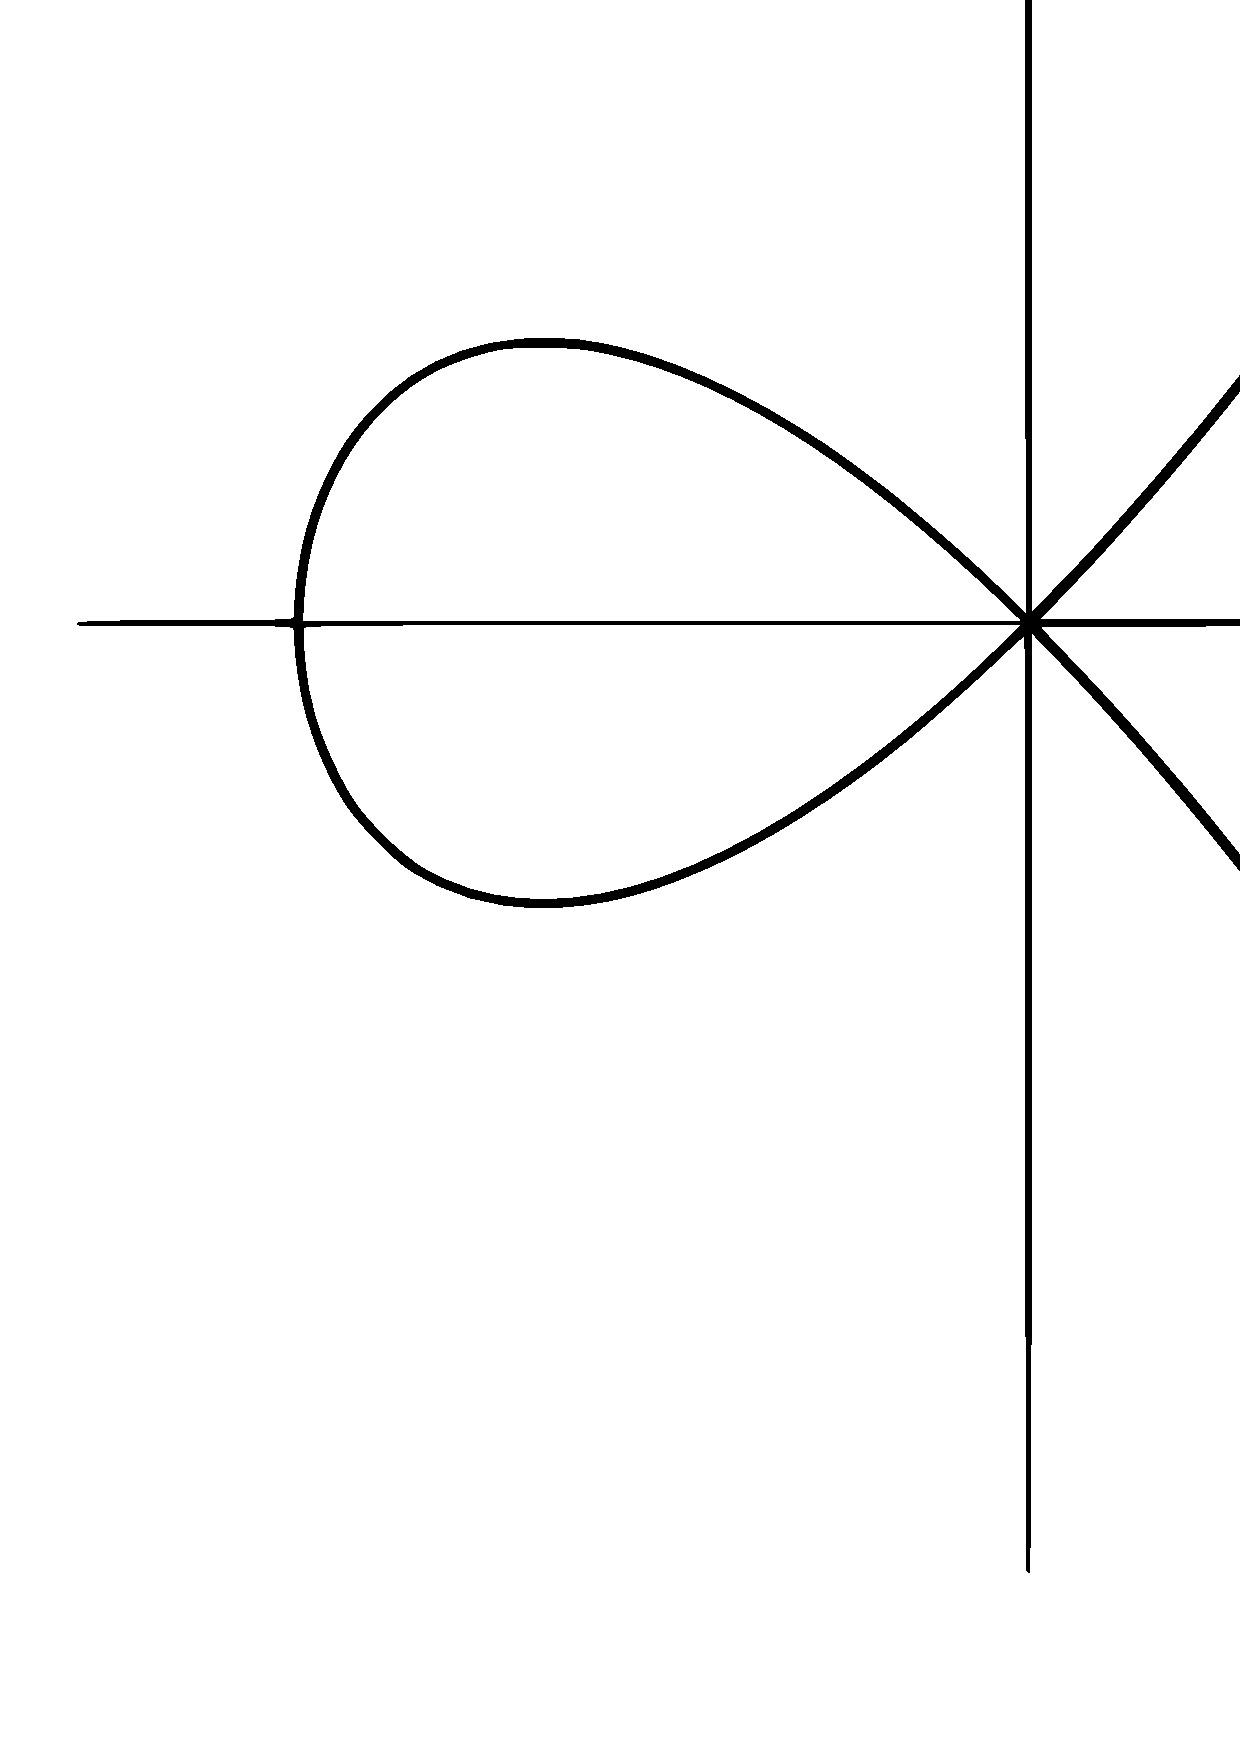
\includegraphics[scale=\scale,bb=0 0 688 413]{\PICDIR/2.png}\end{center}

因为$K[x,y]=K[x]\otimes_K K[y]$,从定义有
\[
	\mathbb{A}^2_K=\mathbb{A}^1_K\times_{\spec K}\mathbb{A}^1_K.
\]
在这里,纤维积显然是一个正确的积,但它作为集合并不等于其因子作为集合的积。

仿射空间$\mathbb{A}^n_K$是上一个例子的直接推广:几何上,可以看到概形$\mathbb{A}^n_K$是经典的仿射$n$-空间对每一个正维数的不可约子簇$\Sigma$加上一点$p_\Sigma$. 与前面一样,$p_\Sigma$属于$\Sigma$的闭包中,且$p_\Sigma$的闭包等于$\Sigma$的闭包,是$\Sigma$的一般点。

更一般的,设$X\subset \mathbb{A}^n_K$是任意的仿射簇,对应于理想$I\subset \mathbb{A}^n_K$以及坐标环$R=K[x_1$, $\dots$, $x_n]/I$,我们能得到对应的仿射概形$\spec R$,并可以通过商映射$K[x_1$, $\dots$, $x_n]\to R$将它看作$\mathbb{A}^n_K$的一个子概形。这个概形,与$\mathbb{A}^n_K$的情形类似,长得就像仿射簇$X$但还需要对每一个正维数的不可约子簇$\Sigma\subset X$加入一个新的一般点$p_\Sigma$.

纤维,或者更一般的原像,是除了簇之外,概形最有可能出现在经典代数几何中的方式。

\begin{exe} \label{exe:2.2}
设$\varphi:K[x]\to K[x]$是一个环同态,他将$x$变成$x^2$,考虑$\varphi$诱导的$\spec K[x]$到自身的映射。证明,在概形意义上,点$0$的纤维是由$(x^2)$定义的子概形。

\begin{center}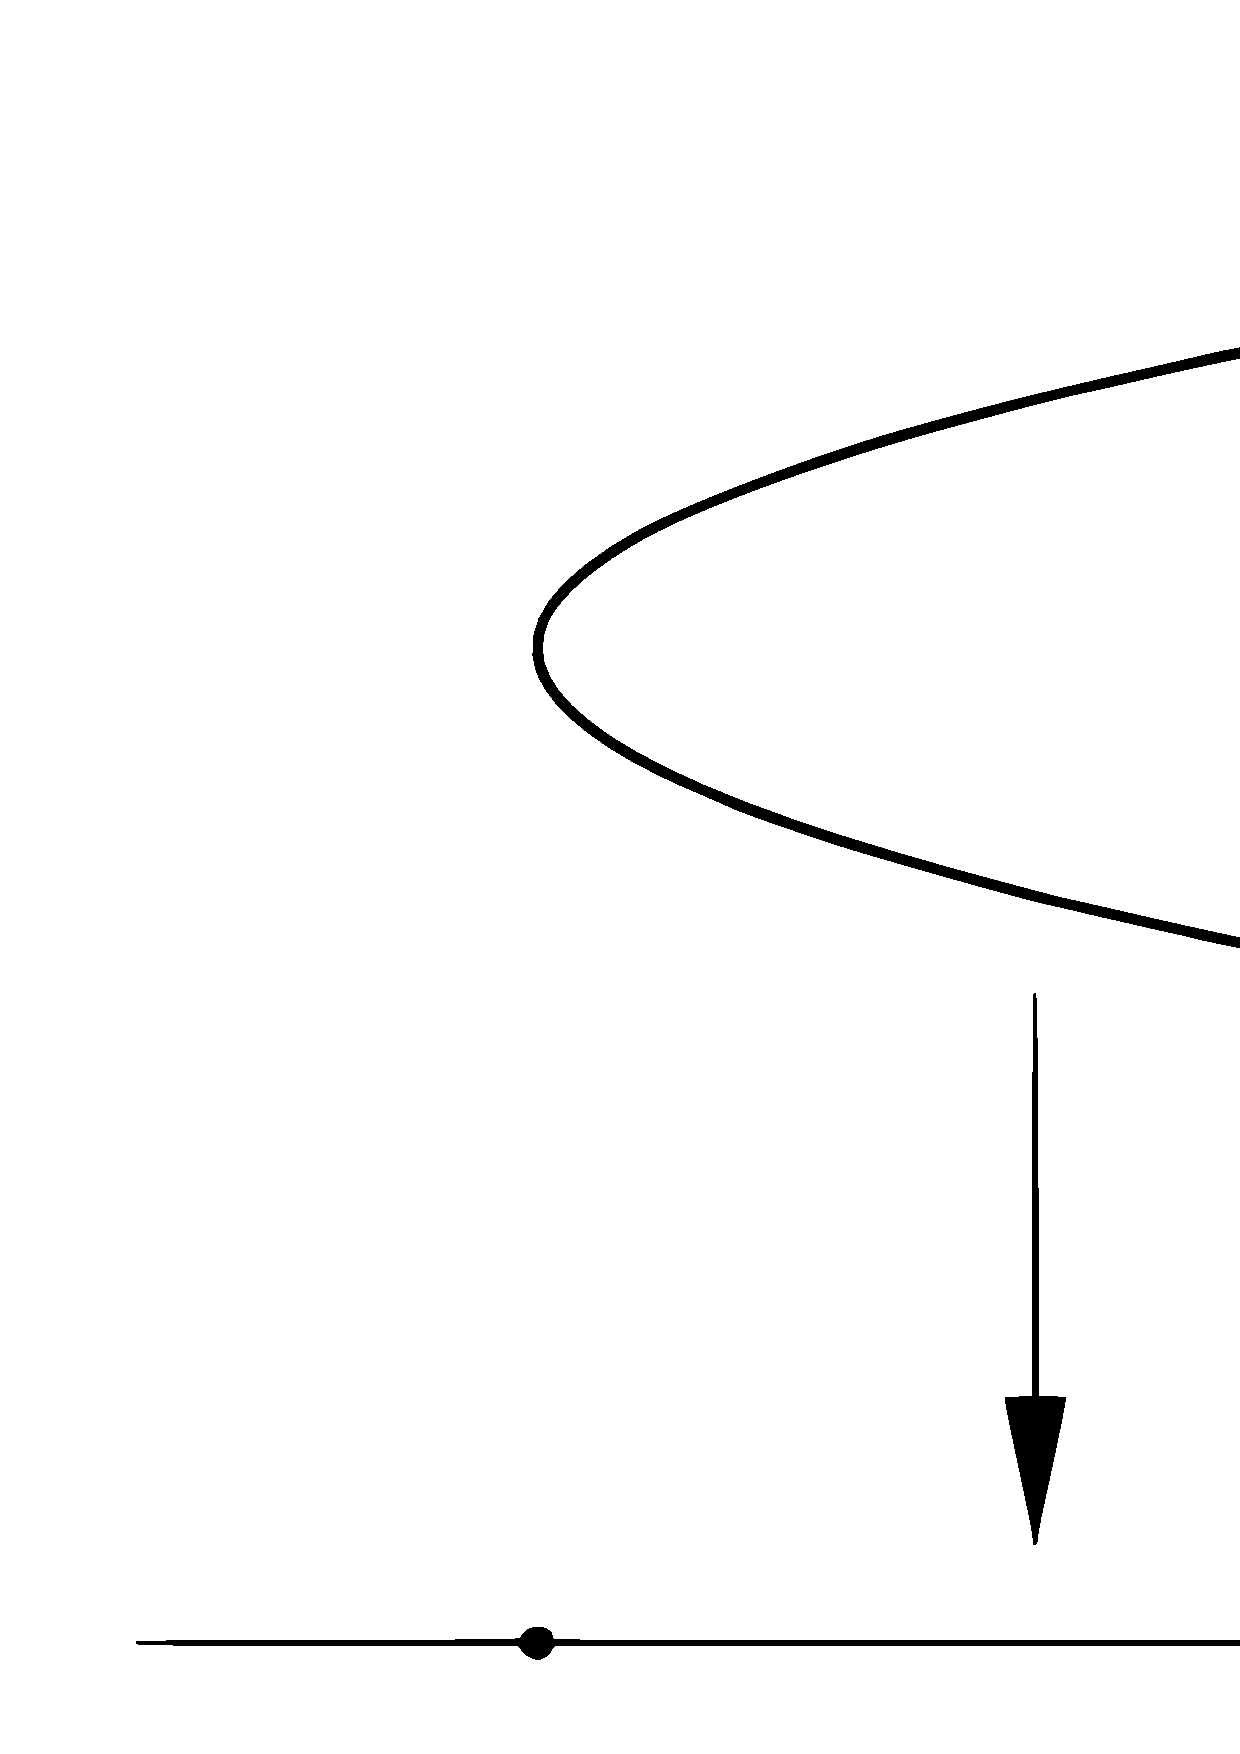
\includegraphics[scale=\scale,bb=0 0 507 309]{\PICDIR/3.png}\end{center}
\end{exe}

在所有的概形中,代数闭域上仿射簇的相伴概形被如下性质的环$R$的谱所刻划,
\begin{compactitem}[~~~--]
\item 有限生成
\item 约态代数\index{约态!代数}
\item 在一个域上
\item 这个域是代数闭域
\end{compactitem}

为了对更一般的概形长什么样有所感觉,以及对它们有什么益处有所把握,我们在接下来的几节中考虑撤去上面四条限制中的几条后将会发生什么。我们会主要考虑那些上面四条限制中只有一条不满足的情况,因为理解它们将帮助我们理解更一般的情况;在习题中,偶尔会提到更复杂的例子。

\subsection{局部概形}

我们的第一类不同于簇的概形的例子是局部环的谱,称之为\textit{局部概形}\index{局部!概形}。我们这里将考虑的例子是代数闭域上约态代数的谱,但不一定是有限生成的。局部概形常常作为技术性工具来研究其他更几何的概形:它们经常被用来关注仿射概形的局部结构上。在只有一个闭点的例子中,概形比起簇新增的点将变得更加醒目。自然,只用一个几何点来表示这些概形是错误的,取而代之的,它们应当被看成簇的芽。只有一个闭点的现象不是新近才被代数学家研究的,作为类似物,当考虑复解析流形上一点处的芽时它已经出现了,那里它给出了一点$x$处“足够小”的邻域的图像:比如,在这个“足够小”的邻域中,每条经过$x$的曲线都可以被区分开来,尽管它们可能除了$x$之外再无在任意的邻域中有定义的点。在局部环的谱上,我们将看到类似的图像。

首先考虑环$K[x]$关于极大理想$(x)$的局部化$K[x]_{(x)}$,令$X=\spec K[x]_{(x)}$. 空间$|X|$只有两个点:一个闭点对应于极大理想$(x)$,另一个开点对应于零理想$(0)$,他的闭包包含点$(x)$. 含入同态$K[x]\hookrightarrow K[x]_{(x)}$诱导了一个映射$X\to \mathbb{A}_K^1$,于是我们将$X$看作$\mathbb{A}_K^1$的子概形(尽管$|X|$在$\mathbb{A}_K^1$不是开的也不是闭的)。子概形$X$是“局部的”,因为$X$是所有$\mathbb{A}_K^1$中包含$(x)$的开集的交%
\footnote{译者注:若一个拓扑空间存在一般点,则其任意开子集都包含所有的一般点。设$\mathbb{A}_K^1$中所有包含$(x)$的开集的交为$U$,因此$X=\{(0),(x)\}\subset U$. 反过来,对任意闭点$p\in \mathbb{A}_K^1$,则$\mathbb{A}_K^1-p$是一个包含$(x)$的开集,但是并不包含$p$,所以$p\not\in U$. 于是$X=U$. 这个命题可以如下推广:设$X$是一个拓扑空间,对$x\in X$,记所有$x$的开邻域的交为$S_x$,则$S_x=\{y\,:\, x\in \overline{\{y\}}\}$.}%
,于是,比如,$X$上的正则函数正好就是$\mathbb{A}_K^1$上在点$0=(x)$处正则的有理函数,即它们是$\mathscr{O}_{\mathbb{A}_K^1}(U)$中的元素,其中$U$是$\mathbb{A}_K^1$中包含点$0=(x)$的某个邻域。在这层意味上,$X$是$\mathbb{A}_K^1$在原点处的芽。

接着,考虑概形$X=\spec R$,其中$R=K[x,y]_{(x,y)}$是$K[x,y]$关于极大理想$(x,y)$的局部化,极大理想$(x,y)$对应于点$(0,0)$. 同上,我们有映射$X\to \mathbb{A}_K^2$,这里我们能将$X$看成$\mathbb{A}_K^2$中所有$(0,0)$的邻域的交。类似地,$X$只有一个闭点,但现在却有了无穷多的非闭点,每一个都对应于一条经过原点的不可约曲线。于是,$X$的子概形是$\mathbb{A}_K^2$的子概形在$(0,0)$的芽,以及$X$本身是$\mathbb{A}_K^2$在$(0,0)$的芽。

对$\mathbb{A}_K^n$乃至对$\mathbb{A}_K^n$的每一个子概形,都有类似的构造:如果$X=\spec K[x_1,$ $\dots$, $x_n]/I\subset \mathbb{A}_K^n$是一个理想为$I$的仿射簇的相伴概形,而$\mathfrak{m}$对应于$X$的一个闭点,我们能将概形$\spec K[x_1,$ $\dots$, $x_n]_\mathfrak{m}/I_{\mathfrak{m}}$看成$X$中$[\mathfrak{m}]$的一个邻域的芽。与在许多语境中谈论一个空间上一点处的函数芽不同,在概形理论中,芽依然是一个概形。

在某些场合,这样引入的局部概形实际上还不够局部:概形一点处的局部环依然包含着许多概形整体结构的信息。比如,非奇异簇$X$的概形在不同闭点处的芽不一定是同构的,尽管当我们考虑由同一个方程定义的复解析簇$X^{\text{an}}$时,任意两点的芽确实是同构的。出现这个现象的实质在于这里用来定义芽的开集太大了。为了在概形语境下得到一个更局部的图像,我们需要观察幂级数环对应的概形:比如,比起考察$\mathbb{A}_K^2$处原点$(0,0)$某个邻域的芽$X=\spec K[x,y]_{(x,y)}$,我们转而考虑概形$Y=\spec K [\![x,y]\!]$. 与前面的例子类似,它只有一个闭点$[(x,y)]$以及一个一般点$[(0)]$,一般点的闭包是整个$Y$,此外,对每一个$x$和$y$的不可约幂级数$\sum a_{i,j}x^iy^j$,$Y$上都对应着有一点。映射 %proofread
\[
	K[x,y]\hookrightarrow K[x,y]_{(x,y)}\hookrightarrow K[\![x,y]\!]
\]
给出了映射$Y\to X\to \mathbb{A}_K^2$,于是我们能把$Y$想象成比$X$“更小的”原点的邻域。(然而,注意到$X$和$Y$都不是$\mathbb{A}_K^2$的开子概形或闭子概形。)比如,如果$X$中对应于素理想$(y^2-x^3-x^2)$的曲线是不可约,且域$K$的特征不是$2$,则$\mathbb{A}_K^2$中被这个方程定义的曲线在$Y$中的原像是两个(非平凡)曲线的并。因为$x^2+x^3$有着幂级数表示的平方根
\[
	u=x+\frac{1}{2}x^2-\frac{1}{8}x^3+\cdots.
\]
因此我们能把$y^2-x^3-x^2$分解为
\[
	y^2-x^3-x^2=(y-u)(y+u),
\]
所以概形$\spec  K[\![x,y]\!]/(y^2-x^3-x^2)$是可约的。(见下图。)

\begin{center}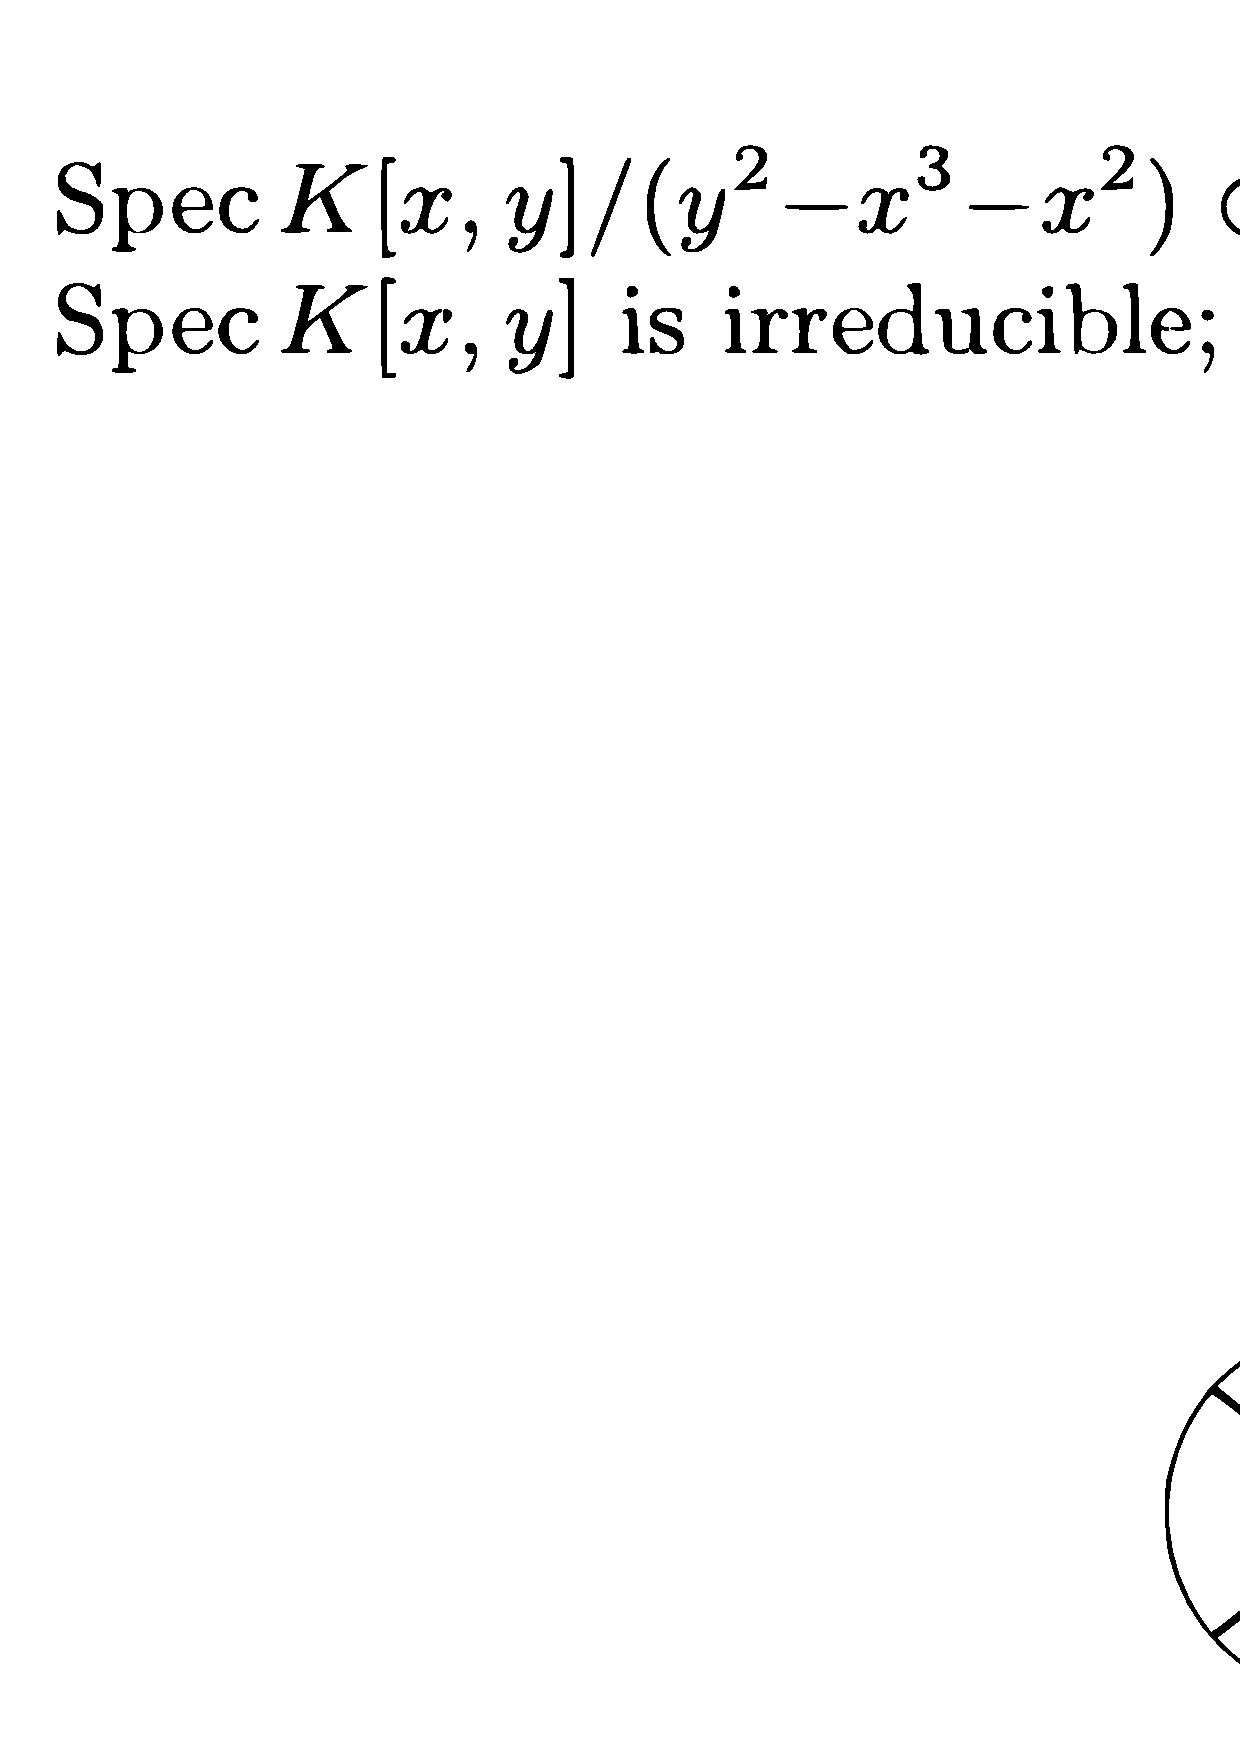
\includegraphics[scale=\scale,bb=0 0 600 444]{\PICDIR/4.png}\end{center}

当然,为使这样的事是可行的,$Y$必然比$X$有“更多”曲线,下面的习题补充了这点。

\begin{exe}
	\begin{compactenum}[(a)]
		\item 同上,设$u=\sqrt{x^2+x^3}$,那么$[(y-u)]$在$\spec K[x,y]$中的像是什么?(提示:这是一个包含$y^2-x^3-x^2$的素理想。)
		\item 证明,$Y$中的点$(y-\sum_{n\geq 1}x^n/n!)$在$\mathbb{A}_K^2$中的像是$\mathbb{A}_K^2$的一般点。
	\end{compactenum}
\end{exe}

一般地,在上面的映射$Y\to X$下,一点的原像对应于一条$\mathbb{A}_K^2$的不可约曲线$C$,它由原点处$C$的所有解析分支构成。(更多关于分支的讨论见Walker [1950]或者Brieskorn以及Kn\"{o}rrer [1986].)

虽然这里有了局部概形的另一个重要例子,但上面的概形$Y$的一个问题是,Exercise {\theexe}(b)中的点与代数的观点相去甚远。为了避免这点,我们可以转而考虑幂级数环的子环$H\subset K[\![x,y]\!]$的谱$Z$,其中环$H$在$K[x,y]$的分式域$K(x,y)$上满足一个代数方程。我们称其为概形$X$的\idx{Hensel化},概形$Z$居于$Y$与$X$之间,使得我们有一列映射
\[
	Y\to Z\to X\to \mathbb{A}_K^2.
\]
这种构造的用处在于,$H$是一系列有限生成$K$\hyp 代数的并,于是$Z$是一族概形的逆极限,这族概形每一个都来自于寻常的簇。几何上来看,$Z$是在$\mathbb{A}_K^2$在\textit{\'{e}tale拓扑}\index{\'{e}tale!拓扑}下的芽。这个概念我们这里按下不表,详细可见Artin [1971].

\begin{exe}
	当$K=\mathbb{C}$,如何将收敛幂级数构成的环的谱纳入这种图像中?
\end{exe}
\section{非代数闭域上的约态概形}

现在我们考虑当观察非代数闭域上的有限生成约态代数\index{约态!代数}的谱时将会发生什么。对这样的结构的兴趣最早来自于数论,当然,它远比概形理论要早得多!比如,关于有理二次型的研究,这是数论中一个古老的课题,能看作对有理数域上二次方程定义的簇的研究。研究有理数域上三个变量的三次型在数论上至今依然是非常活跃的方向,其中现在主要醉心于$\mathbb{Q}$上的椭圆曲线理论。虽然这里最基本的对象是$\mathbb{Q}$上的代数簇(或是$\mathbb{Z}$上的概形,我们以后会回到这个情况),但在处理它们的过程中,数论学家常常使用下面这副图中这些所有的基环,以及许多的中间域以及中间环:
\[
\begin{xy}
	\xymatrix{
		\hat{\mathbb{Z}}_{(p)}\ar[r]&\hat{\mathbb{Q}}_{p}\ar[rr]&&\mathbb{C}_p\\
		\mathbb{Z}_{(p)}\ar[u]&&&\\
		\mathbb{Z}\ar[u]\ar[r]\ar[d]&\mathbb{Q}\ar[r]\ar[uu]&\mathbb{R}\ar[r]&\mathbb{C}\ar[uu]\\
		\mathbb{F}_p\ar[r]&\bar{\mathbb{F}}_p&&&
	}
\end{xy}
\]
概形理论提供了一个相当富有弹性且舒适的框架来处理这些基环的改变。此外,一个性质良好的约态簇,在模$p$后可能突然变成一个非约态的东西,描述这东西需要更完整的概形理论(比如见第 \ref{s:2.4.4} 小节)。

从最简单的例子开始,考虑$\mathbb{A}_{\mathbb{R}}^1=\spec \mathbb{R}[x]$. 使用Nullstellensatz,可以看到$R[x]$中有两类极大理想:一类的剩余类域是$\mathbb{R}$,它们具有形式$(x-\lambda)$,其中$\lambda\in\mathbb{R}$,剩余类域是$\mathbb{C}$,它们具有形式$(x^2+\mu x+\nu)$,其中$\mu$, $\nu\in\mathbb{R}$且满足$\mu^2-4\nu<0$. 另一类理想可以写作$((x-z)(x-\bar{z}))$的形式,其中$z\in \mathbb{C}$不是一个实数。于是,$\mathbb{A}_{\mathbb{R}}^1$中的闭点,对应于一个实数或者一对共轭的复数。最后,$\mathbb{A}_{\mathbb{R}}^1$同样有着唯一的非闭点,对应于素理想$(0)$,它的闭包是整个$\mathbb{A}_{\mathbb{R}}^1$.

接着,我们来到$\mathbb{R}$上的仿射平面,$\mathbb{A}_{\mathbb{R}}^2=\spec \mathbb{R}[x,y]$,以及考虑$R[x,y]$的极大理想$\mathfrak{m}$给出的闭点。同样从Nullstellensatz,$R[x,y]$关于$\mathfrak{m}$的剩余类域只有$\mathbb{R}$与$\mathbb{C}$,于是复合映射
\[
	\rr\to \rr[x,y]/\mm\cong (\rr \text{ or } \cc)
\]
或者是恒同或者是$\rr$到$\cc$的含入。取$\lambda$和$\mu$作为$x$和$y$在$\cc$中的像,对前一种情况,我们可以看到$\mm=(x-\lambda,y-\mu)$对应于$\rr^2$中一般意义上的点。但是对后一种情况,$\mm$同时对应于$(\lambda,\mu)$和$(\bar\lambda,\bar\mu)$:从另一种视角来看,将$x$, $y$变成$\lambda$, $\mu$的同态$\rr[x,y]\to \cc$与另一个将$x$, $y$变成$\bar\lambda$, $\bar\mu$的同态有着相同的核,因为它们只差一个$\cc$在$\rr$上的自同构。

给出上面描述的极大理想的生成元并不是件很困难的事情。如果$\rr[x,y]/\mm\cong \rr $,很清楚地,$\mm=(x-\lambda,y-\mu)$. 另一方面,假设$\lambda$是实数,则$\mu$必须要满足一个不可约二次实系数多项式$y^2+ay+b=0$,于是$\mm$包含理想$(x-\lambda,y^2+ay+b)$. 但这个理想显然是一个素理想(比如,先模掉$x-\lambda$因子),于是$\mm=(x-\lambda,y^2+ay+b)$. 自然,当$\mu$是实数的时候,类似的结果也成立。

最后,假设$\mu$和$\lambda$都不是实数,于是$\mm$包含以$\mu$和$\lambda$为根的不可约实系数多项式$f$和$g$,但是,因为$g$可以在$\rr[x]/(f(x))\cong \cc$上分解为
\[
	g(y)=(y-\mu)(y-\bar\mu),
\]
因此$(f(x),g(y))$不是素理想!在复数域上,可以给出如下图像:

\begin{center}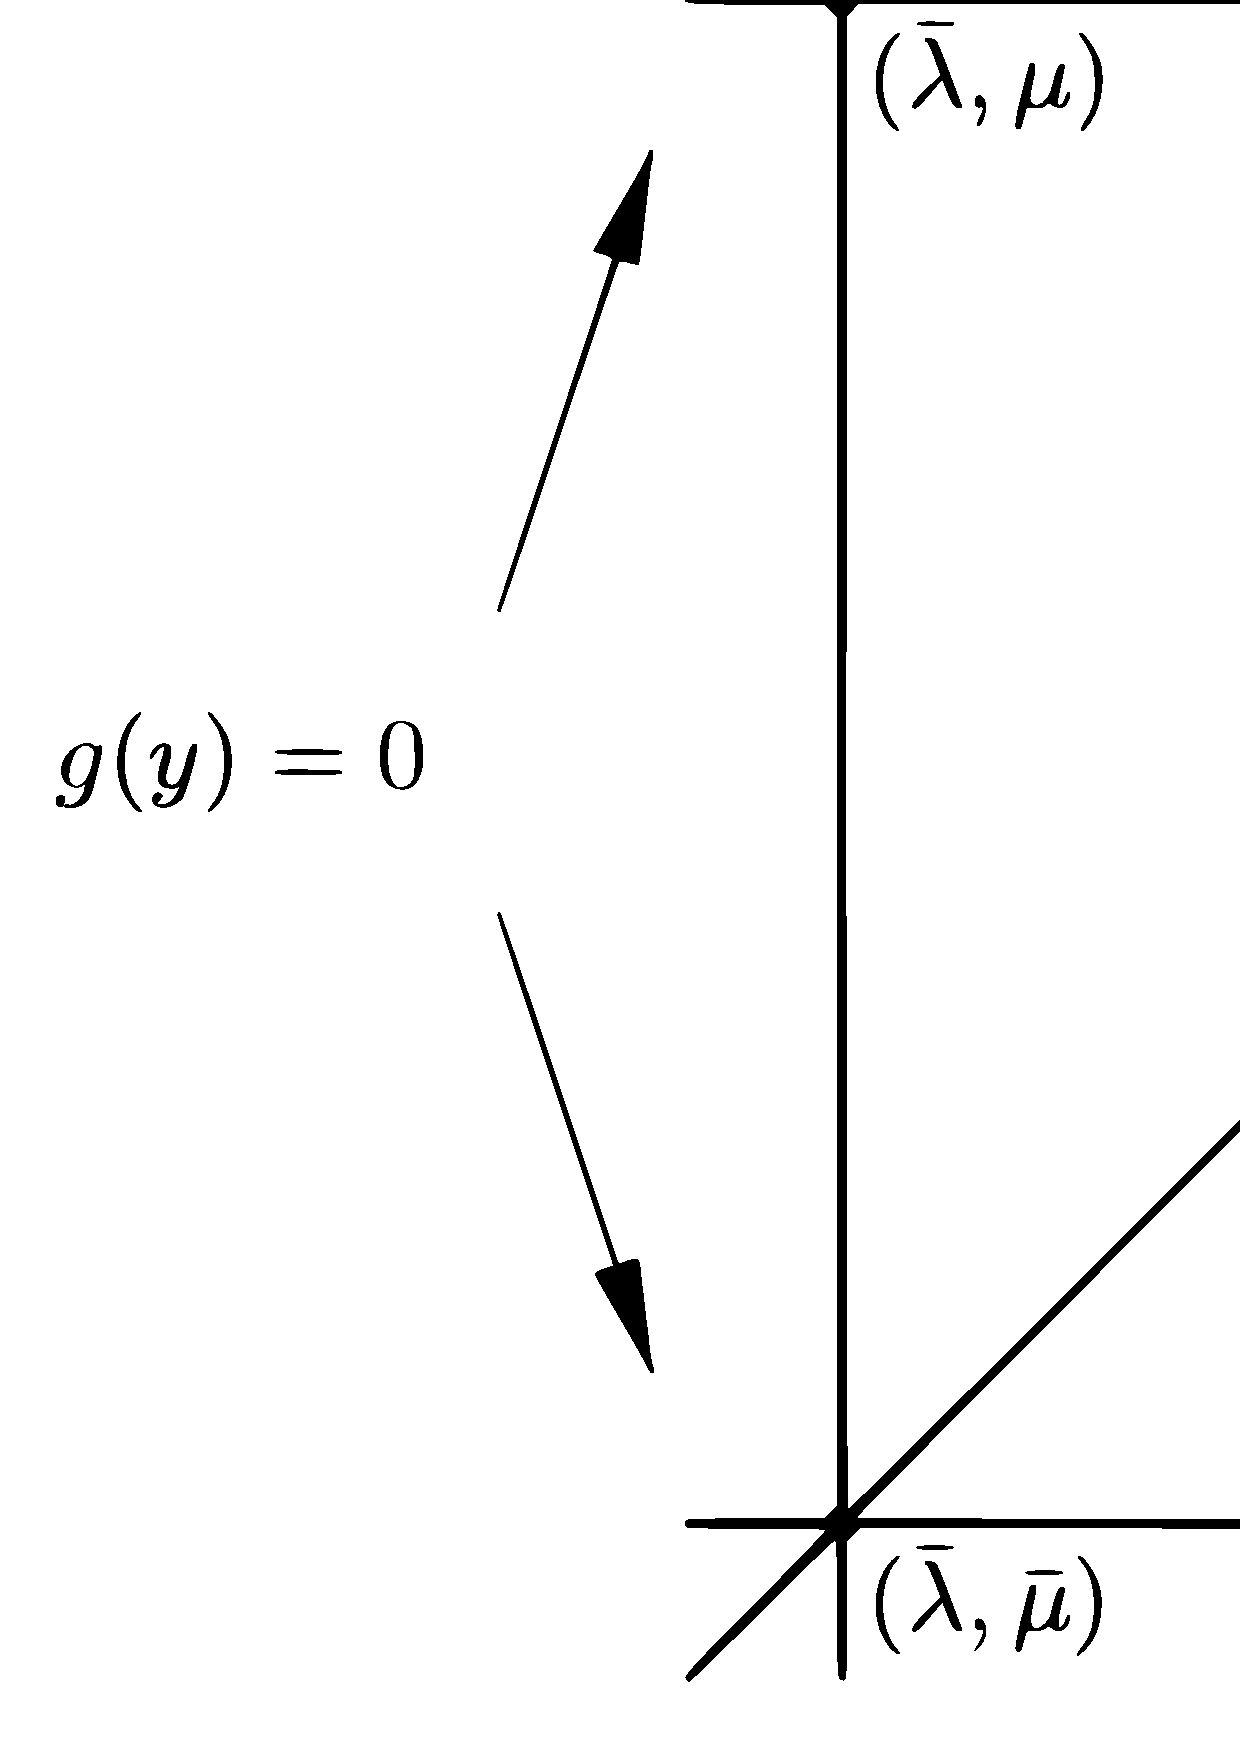
\includegraphics[scale=\scale,bb=0 0 683 419]{\PICDIR/5.png}\end{center}

$f(x)=0$与$g(y)=0$的零点集分别是两条水平线与数值线的并,它们相交于四点$(\lambda,\mu)$, $(\bar\lambda,\mu)$, $(\lambda,\bar\mu)$和$(\bar\lambda,\bar\mu)$. 多项式
\[
	h(x,y)=\mathrm{Im}(\mu) x - \mathrm{Im}(\lambda)  y -\mathrm{Im}(\mu\bar\lambda)
\]
是连接$(\lambda,\mu)$和$(\bar\lambda,\bar\mu)$的那条实系数直线。理想
\[
	(f(x),h(x,y))=(g(y),h(x,y))\subset \rr[x,y]
\]
严格包含理想$(f(x),g(y))$,它就是我们寻找的极大理想,这点可以通过检查
\[
	\rr[x]\cong \rr[x,y]/(h)\cong \rr[y]
\]
得到(这些同构中,注意到$(\bar\mu-\mu)$与$(\bar\lambda-\lambda)$都非零)。

总之,$\mathbb{A}_{\rr}^2$的闭点集,对应于$\mathbb{A}_{\cc}^2$中的点$(\lambda,\mu)$,其中$\lambda$和$\mu$都是实数,或者对应于(无序)偶对$(z,w)$或者$(\bar z,\bar w)\in \mathbb{A}_{\cc}^2$,其中$z$, $w$至少有一个不是实数。从另一种角度来看,$\mathbb{A}_{\rr}^2$的闭点对应于$\mathbb{A}_{\cc}^2$中点共轭作用后的轨道。(注意,特别地,$\mathbb{A}_{\rr}^2$的闭点不是$\mathbb{A}_{\rr}^1$中闭点的有序偶对!)同样可以注意到,$\mathbb{A}_{\rr}^2$中点$(\lambda,\mu)$处的剩余类域是$\rr$,其中$\lambda$, $\mu$都是实数,而$\mathbb{A}_{\rr}^2$中复共轭的一对点处的剩余类域是$\cc$.

\begin{exe}
	证明$\mathbb{A}^2_{\rr}$的全部非闭点是
	\begin{compactenum}[(a)]
		\item $[(0)]$,它的闭包是整个$\mathbb{A}^2_{\rr}$,或者
		\item 点$[(f)]\in \mathbb{A}^2_{\rr}$对应于不可约多项式$f\in \rr[x,y]$.
	\end{compactenum}

	上面的(b)类点的多项式在$\cc[x,y]$中不一定还是不可约的,故$\mathbb{A}^2_{\rr}$中的非闭点$(f)$会对应于$\mathbb{A}^2_{\cc}$的一个非闭点($f$在$\cc[x,y]$中还是不可约的)或者两个非闭点($f$在$\cc[x,y]$能写成乘积$g\bar g$,其中$g\in\cc[x,y]$). 这样的非闭点的闭包中的闭点,要么上面的第一类第二类都有,要么只有第二类。试给出所有这些可能性的例子。
\end{exe}

一般的情况按下面这列例子进行:如果$K$是任意的域,$\bar K$是它的代数闭包,而$G=\mathrm{Gal}(\bar K/K)$是对应的Galois群,则$\mathbb{A}_{K}^n$中的点对应于$G$作用在$\mathbb{A}_{\bar K}^n$上的点的轨道(比如见Nagata [1962, Theorem 10.3])。闭点对应于闭点的轨道,而轨道是有限的。点$p$处的剩余类域,对应于在某条轨道上使其一点不动的子群$G_p$作用在$\bar K$上的不变域。比如,$\mathbb{A}^1_\mathbb{Q}$的闭点对应于代数数模掉共轭;以及对素数$q\in \mathbb{Z}$,$\mathbb{A}_{\mathbb{F}_q}^1$的闭点对应于$\mathbb{F}_q=\mathbb{Z}/(q)$的代数闭包的Frobenius自同构的轨道(即,$0$以及映射$a\mapsto a^q$在乘法群$\bar K^*$上的轨道,也能被描述为所有阶数与$q$互素的循环群的归纳极限,或者是$\mathbb{Q}/\mathbb{Z}$的$q$-无挠部分)。

\begin{exe}
	域的含入映射$K\hookrightarrow L$诱导了映射$\mathbb{A}_L^n\to \mathbb{A}_K^n$. 找出下面这些$\mathbb{A}_{\overline{\mathbb{Q}}}^n$的点在这个映射下在$\mathbb{A}_{\mathbb{Q}}^n$中的像。
	\begin{compactenum}[(a)]
		\item $(x-\sqrt{2},y-\sqrt{2})$
		\item $(x-\sqrt{2},y-\sqrt{3})$
		\item $(x-\zeta,y-\zeta^{-1})$,其中$\zeta$是$p$次单位根,而$p$是一个素数
		\item $(\sqrt{2}x-\sqrt{3}y)$
		\item $(\sqrt{2}x-\sqrt{3}y-1)$
	\end{compactenum}
	如果可能则做出图像。
\end{exe}

\begin{exe}
	我们说子概形$X\subset \mathbb{A}_K^n$是\textit{绝对不可约的}\index{不可约!绝对}或者是\textit{几何不可约的}如果$X$在$\mathbb{A}_{\bar K}^n$中的原像是不可约的。(更一般地,我们说任意$K$\hyp 概形$X$是绝对不可约的如果纤维积$X\times_{\spec K}\spec \bar{K}$是不可约的。)将下面这些$\mathbb{A}_\mathbb{Q}^2=\spec \mathbb{Q}[x,y]$的子概形分类成可约的、不可约但不是绝对不可约的或者绝对不可约的。
	\begin{compactenum}[(a)]
		\item $V(x^2-y^2)$
		\item $V(x^2+y^2)$
		\item $V(x^2+y^2+1)$
		\item $V(x+y,xy-2)$
		\item $V(x^2-2y^2,x^3+3y^3)$
	\end{compactenum}
\end{exe}

最后,这里有一个联合了局部概形与非代数闭域上的概形两个概念的例子。经典地,对平面曲线$X\subset \mathbb{A}_\cc^2$,如果在原点处有一个解析邻域,使得在其中$Y$的复点的轨迹\footnote{译者注:原文是``if in some analytic neighborhood of the origin the locus of complex points of $Y$''. $Y$似乎应该理解成$X$在这个解析邻域里面的像。复点的意思在后文才被揭示,是在那里剩余类域为$\cc$的点。 ``locus''请允许我翻译成轨迹,其实想象成这些点的集合就行,毕竟是经典图像。}$Y$由两条在$(0,0)$处横截相交的光滑弧构成,则$X$被称为在原点处有一个\idx{结点}(node)。在概形的语言中,这等价于说,$X$与形式邻域$\spec \cc[\![x,y]\!]\to \spec \cc[x,y]=\mathbb{A}_\cc^2$的纤维积同构于$\spec \cc[\![u,v]\!]/(uv)$.

现在考虑实平面上的曲线$X\subset \mathbb{A}_\rr^2$. 这种情况下,我们称$X$在原点处有一个结点,如果对应的复曲线
\[
	X\times_{\spec \rr}\spec \cc \subset \mathbb{A}_\cc^2
\]
在原点处有。在这个例子里,形式邻域
\[
	X\times_{\spec \rr[x,y]}\spec \rr[\![x,y]\!]
\]
可能具有两种形式,同构于$\spec \rr[\![u,v]\!]/(uv)$或同构于$\spec \rr[\![u,v]\!]/(u^2+v^2)$,这两种形式不同构。前一种情况是如果$X$的实点的轨迹(即剩余类域为$\rr$的点的轨迹)在$(0,0)$的解析邻域中看上去像是两条光滑实弧线横截相交,经典地,这样的点被称为$X$的\idx{叉点}(acrunode)。后一种情况是原点作为$X$的实点被孤立了,这样点以前被称为\idx{孤立点}(acnode)。

\begin{exe}
	验证上面的断言:明确来说,证明如果$\mathbb{A}_\cc^2$中的曲线$X$在原点处有一个结点,则形式邻域$X\times_{\spec \cc[x,y]}\spec \cc[\![x,y]\!]$同构于$\spec\cc[\![x,y]\!]/(uv)$;以及,如果$X\subset \mathbb{A}_{\rr}^2$是一个在原点处有结点的实曲线,那么形式邻域$X\times_{\spec \rr[x,y]}\spec \rr[\![x,y]\!]$是上面提到的两种形式中的一个。证明,存在无限多在原点有结点的曲线$X\subset \mathbb{A}_{\mathbb{Q}}^2$有着不同构的形式邻域。(正如实数情况,我们称$X\subset \mathbb{A}^2_\mathbb{Q}$在原点处有结点,如果对应的复曲线$X\times_{\spec \mathbb{Q}} \spec \cc$有。)
\end{exe}
\section{非约态概形}

我们现在离开那些能被看作概形的对象,即那些仿射概形$\spec R$而$R$是有一个有限生成代数闭域上的代数,且没有幂零元。这里的现象将变得不再那么熟悉,我们需要在他们身上花费更多努力。

这类概形在一些足够简单的几何背景下就已经出现了:比如,下面处理的多重点已经作为两个寻常概形的相交或者作为映射“退化的”纤维出现了,正如Exercise \ref{exe.2.2}中看到的。另一类非约态概形重要的应用在一族簇的理论(theory of families of varieties):形变理论(deformation theory)以及模理论(moduli theory)。我们将解释如何对一族单参数的簇取极限,以及引入平坦性这一关键概念。最后,我们将给出一些非约态概形的例子,这些例子就它们自身而言都是有趣的对象。

从最简单的情况入手,我们将关注仿射空间$\mathbb{A}_K^n$的子概形,其支撑于原点\footnote{译者注:即其支撑只有这点。} ------ 等价地,它由一个理想$I$给出,其零点集$V(I)$作为集合只包含$(0$, $\dots$, $0)$. (回忆一个概形的支撑是指它自有的那个拓扑空间。)

\subsection{双重点}
\index{双重!点}
\begin{exa}
	此类概形最简单的例子是$\mathbb{A}_K^1$由理想$(x^2)$定义的子概形 ------ 即概形$\spec K[x]/(x^2)$,通过商映射$K[x]\to K[x]/(x^2)$诱导的映射看作$\mathbb{A}_K^1$的子概形。这个概形只有一个点,对应于理想$(x)$,但同样作为$\mathbb{A}_K^1$的子概形与作为抽象概形,这与概形$\spec K[x]/(x)=\spec K$不同。作为抽象概形,我们能看到存在如下差别,在$X$上存在非零正则函数(比如$x$)在$X$唯一一点处为零,当然任意这样的函数平方为零。差别在于,作为$\mathbb{A}_K^1$的子概形,$\mathbb{A}_K^1$上的函数$f\in K[x]$在$X$上为零当且仅当$f$和它的一阶导数同时在点$0$为零。于是$X$上的函数包含两个数据,$\mathbb{A}_K^1$上的一个函数与它的一阶导数在点$0$的值。因为这个原因,有时我们将$X$叫做$\mathbb{A}_K^1$中点$0$的\textit{一阶邻域}\index{一阶!邻域}。
\end{exa}

更一般的,对于任意的$n$,理想$(x^n)$定义了一个子概形$X\subset \mathbb{A}_K^1$,它的坐标环为$K[x]/(x^n)$,$\mathbb{A}_K^1$上的函数$f(x)$在$X$上为零当且仅当$f$以及它的前$n-1$阶导数全都在点$0$处为零。

\begin{exa}[双重点]
理解双重点的下一步是考虑$\mathbb{A}_K^2=\spec K[x,y]$中支撑于原点的子概形,这个子概形需要同构于Example {{\addtocounter{thm}{-1}}\thethm{\addtocounter{thm}{1}}}中的那个子概形$X$. 令$Y\subset \mathbb{A}_K^2$是这样的一个子概形,$R=\mathscr{O}_Y(Y)\cong K[\varepsilon]/(\varepsilon^2)$是它的坐标环,以及满射
\[
	\varphi:K[x,y]\to R
\]
定义了$Y$到$\mathbb{A}_K^2$的含入。$R$中唯一的极大理想$\mm$在$K[x,y]$中的原像是对应于原点的理想$(x,y)$,因为在$R$中$\mm^2=0$,所以映射$\varphi$在$(x,y)^2=(x^2,xy,y^2)$上为零,于是诱导了映射
\[
	\bar\varphi:K[x,y]/(x^2,xy,y^2)\to R.
\]
等价地,$Y$必须包含在子概形
\[
	\spec K[x,y]/(x^2,xy,y^2)
\]
中。但环$K[x,y]/(x^2,xy,y^2)$是一个$K$上的三维矢量空间,$R$只有二维。这是因为,$\varphi$的核将包含一个非零齐次线性型$\alpha x+\beta y$,其中$\alpha$, $\beta\in K$. 记
\[
	X_{\alpha,\beta}=\spec K[x,y]/(x^2,xy,y^2,\alpha x+\beta y)\hookrightarrow \mathbb{A}_K^2.
\]
子概形$X_{\alpha,\beta}$能被下面的条件所刻画:

\begin{enumerate}[{(i)}]\setlength{\itemsep}{0pt}
\item 关联于函数$f\in K[x,y]$的理想的$\mathbb{A}^2_K$的子概形,在原点为零以及在那儿其偏导数满足
\[
	\beta\frac{\partial f}{\partial x}-\alpha\frac{\partial f}{\partial y}=0
\]
(因为这可以推出$f=c(\alpha x+\beta y)+\text{高阶项}$),或者
\item Example {{\addtocounter{thm}{-1}}\thethm{\addtocounter{thm}{1}}}中的子概形$X\subset \mathbb{A}_K^1$在$\mathbb{A}_K^1$到$\mathbb{A}_K^2$的含入映射下的像由$x\mapsto (\beta x,-\alpha x)$给出。
\end{enumerate}

经典语言下,子概形$X_{\alpha,\beta}$被称作包含点$(0,0)$以及一个在$\alpha x+\beta y=0$方向上“无穷接近的点”,我们下面在传统图像中以一个小箭头画出$X_{\alpha,\beta}$:

% \pic{6.png}

\noindent 这是打算用一个切空间的可区分的一维子空间在平面上来表示这个点(尽管箭头给出了印象,实际上没有可区分的切矢量)。\nottran
\end{exa}

% \begin{wrapfigure}{i}{140pt}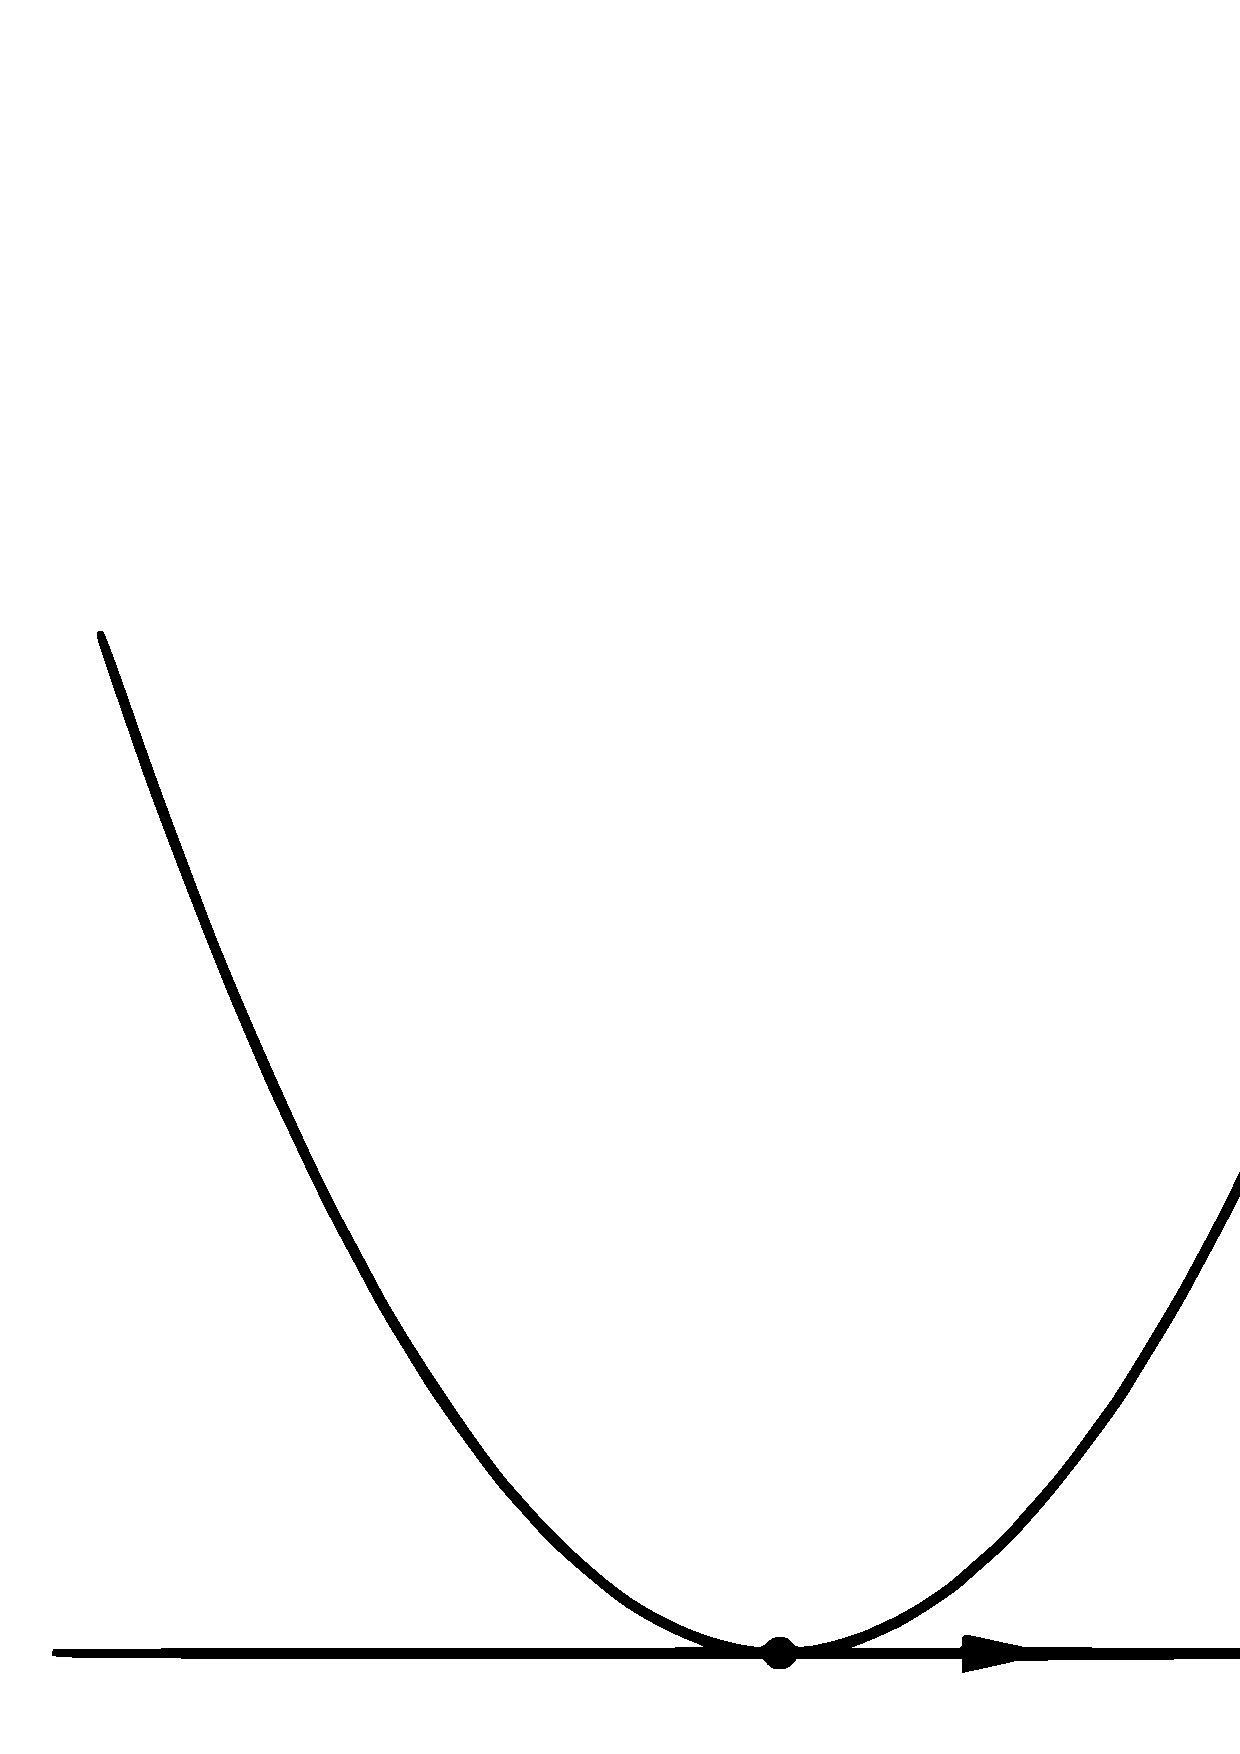
\includegraphics[scale=0.5]{chap_2/pics/7.png}\end{wrapfigure}
在实践中,概形$X_{\alpha,\beta}$会怎么出现呢?一种方式是曲线的相交。比如,当我们想要处理一条直线$L$与一条圆锥曲线$C$相切,显然,只在集合论意义上处理它们的相交是不令人满意的:
一条直线与一条圆锥曲线应该相交两次。甚至,说$C\cap L$的交点“重数为二”也不是完全令人满意的:比如,交点应该决定直线$L$,正如在非相切的例子中那般。真正令人满意的定义是,$C\cap L$是由理想$I_C$与理想$I_L$的和决定的$\mathbb{A}_K^2$的子概形,使得,比如,直线$y=0$以及抛物线$y=x^2$将相交于子概形$X_{0,1}=\spec K[x,y](x^2,y)$. 作为平面中唯一包含于$X_{0,1}$的直线,这将完全决定$L$. 

另一个出现形如$X_{\alpha,\beta}$的子概形的重要方式是作为可约概形的极限。比如,考虑平面上一对不同的点$(0,0)$与$(a,b)$,它们的并是闭子概形
\[
	X=\{(0,0),(a,b)\}=\spec S\subset \mathbb{A}_K^2,
\]
其中
\[
\begin{aligned}
	S&=K[x,y]/\left((x,y)\cap (x-a,y-b)\right)\\
	&=K[x,y]/(x^2-ax,xy-bx,xy-ay,y^2-by).
\end{aligned}
\]
由中国剩余定理,$S\cong K\times K$. 于是,特别地,$S$(作为矢量空间)是一个二维$K$-代数。

现在假设点$(a,b)$沿着一条曲线$(a(t),b(t))$往$(0,0)$移动,其中$(a(0),b(0))=(0,0)$而$a$, $b$是$t$的多项式,我们记作
\[
	a(t)=a_1t+a_2t^2+\dots,\quad b(t)=b_1t+b_2t^2+\dots.
\]

% \begin{center}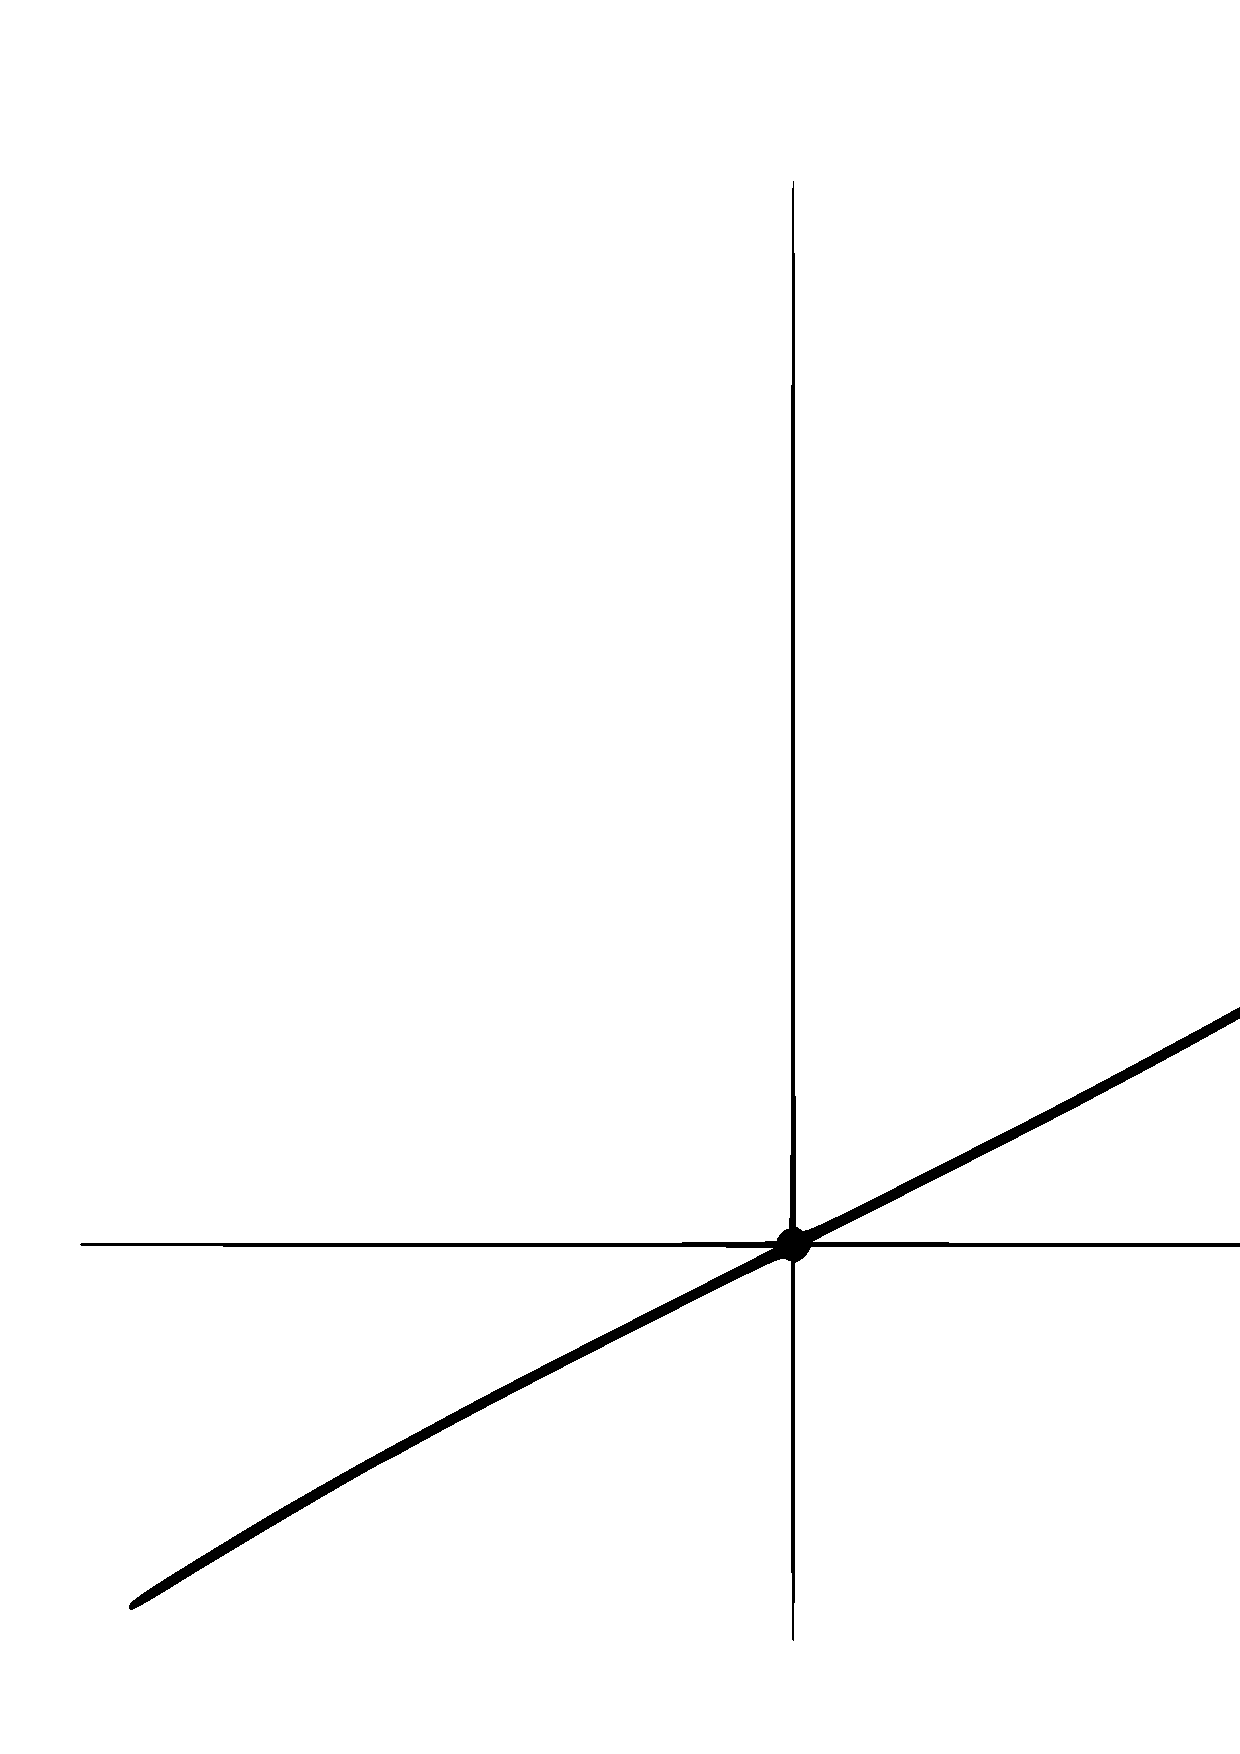
\includegraphics[scale=0.5]{chap_2/pics/8.png}\end{center}

那么$X_t=\{(0,0),(a(t),b(t))\}$在$t\to 0$的极限是什么呢?使用概形,我们能采用一种不常见的观点,在如下的合适表述下,此时它的极限依然是两个点:它将是一个仿射概形$X$,其坐标环依然是一个$K$上的二维矢量空间。我们可以取下面这族理想在$t\to 0$下的极限
\[
	I_t=(x,y)\cap (x-a(t),y-b(t)).
\]
作为关联于$X$的理想来定义$X$. 当然,这仅仅把困难转移到了描述什么是理想族的极限上!但这是简单的:在这个例子中,比如,我们能把它们的极限取为$K[x,y]$
中(看作$K$上的矢量空间时)余维数为$2$的子空间。这个极限依然是一个理想因为乘法是连续的。在理想的余维数是无限时,一个更精巧的解释是必要的,我们将在遇到一维概形族的极限以及再一次在3.3.2节中的射影情况下讨论这个问题。\nottran

为了看看上面说的在实践中是什么意思,首先观察$I_t$生成元$x^2-a(t)x$, $xy-b(t)x$, $xy-a(t)y$以及$y^2-b(t)y$,它们当$t\to 0$的时候有清楚的极限$x^2$, $xy$, $xy$和$y^2$,于是这些多项式应该在$I$中。此外,观察$I_t$包含线性型
\[
	a(t)y-b(t)x=(xy-b(t)x)-(xy-a(t)y),
\]
因此对$t\neq 0$,同样多项式
\[
	\frac{a(t)y-b(t)x}{t}=a_1y-b_1x+t(\dots)
\]
% \begin{wrapfigure}{i}{160pt}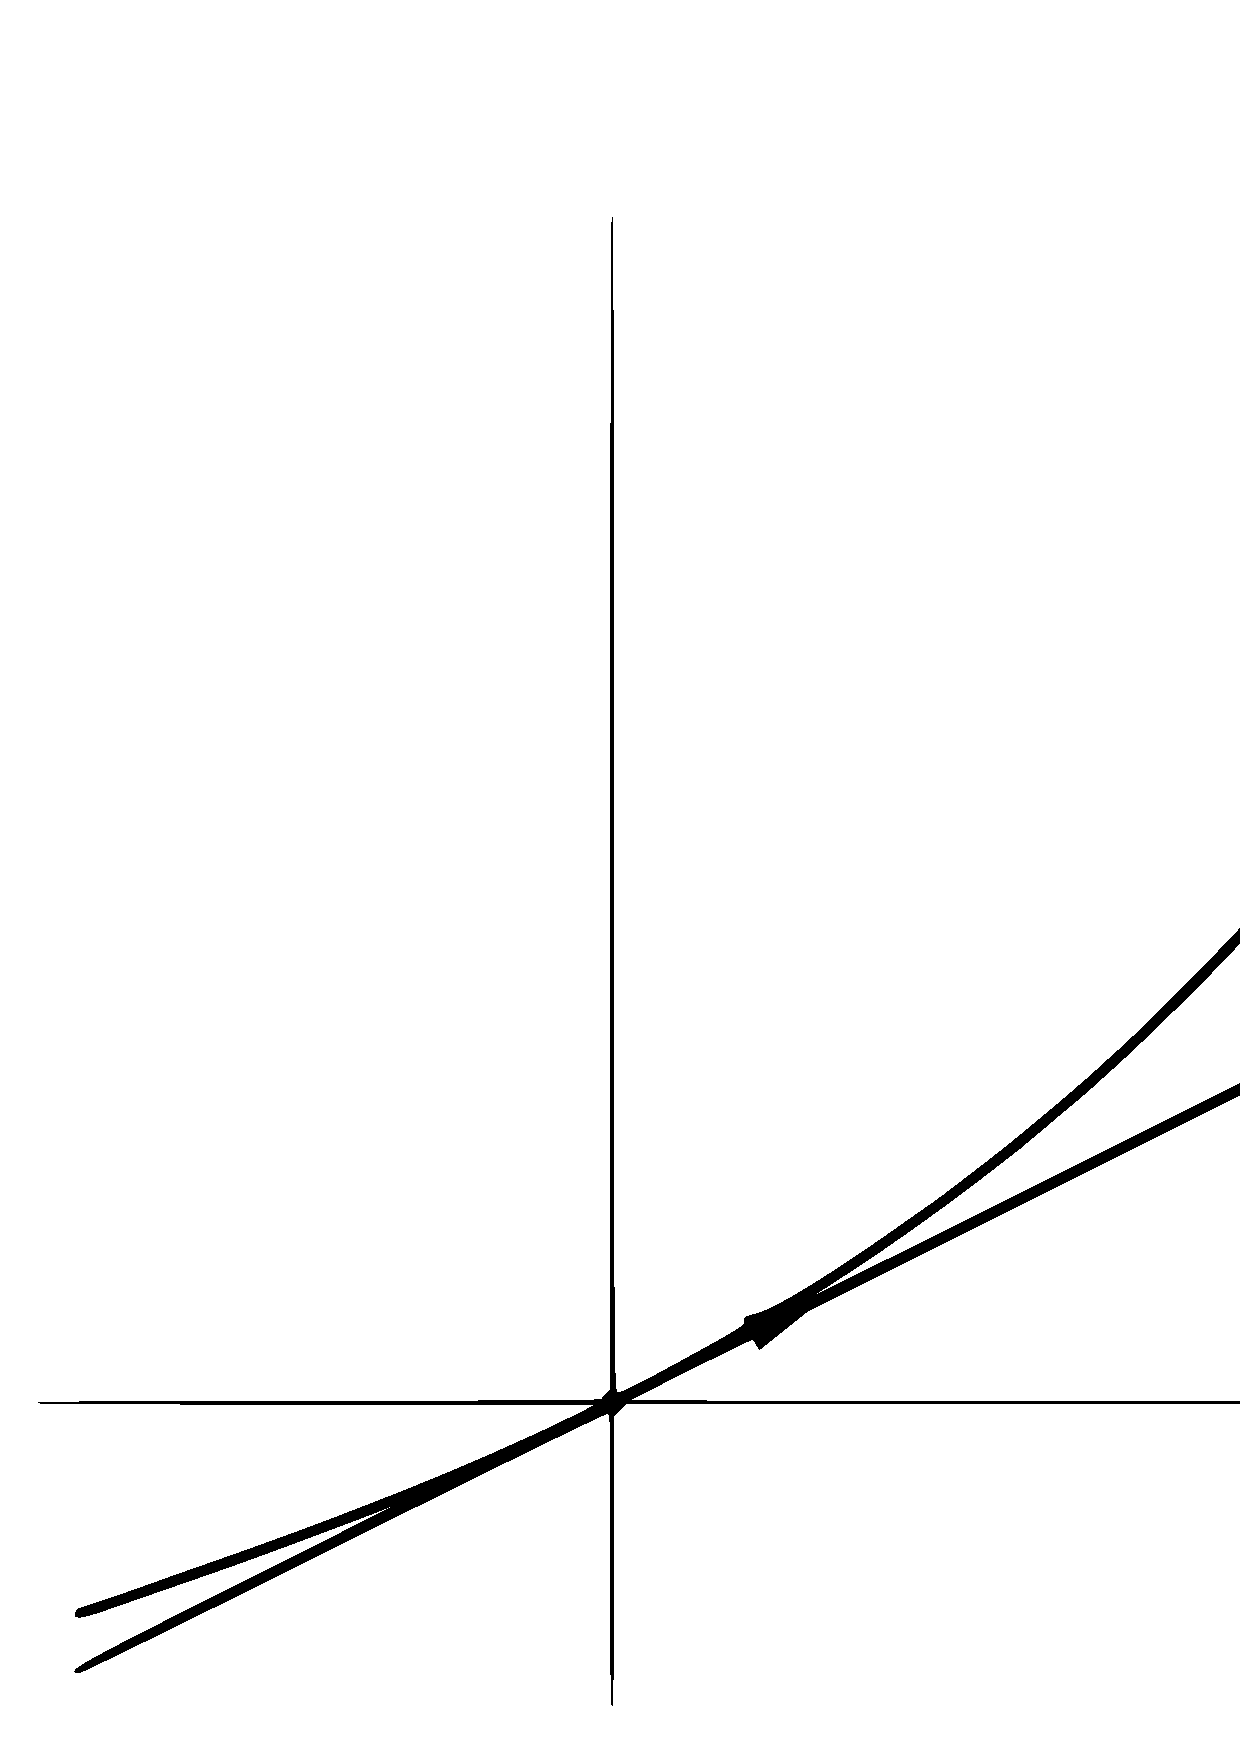
\includegraphics[scale=0.5]{chap_2/pics/9.png}\end{wrapfigure}
也在$I$中。于是,理想$I$同样也包含它的极限$a_1y-b_1x$,于是我们有$I\supset (x^2,xy,y^2,a_1y-b_1x)$. 但是上式右侧作为$K[x,y]$的子空间的余维数已经是$2$了。于是$I=(x^2,xy,y^2,a_1y-b_1x)$,以及,相应地,
\[
	\lim_{t\to 0}(X_t)=X_{\alpha,\beta},
\]
其中$\alpha=b_1$以及$\beta=-a_1$.

从这个例子我们看到,$X$作为$\mathbb{A}_K^2$的子概形,“记住”了$(a(t),b(t))$趋向$(0,0)$的方向:我们认为它包含原点以及原点处沿着直线$a_1y-b_1x=0$的切方向。这条直线是连接$(0,0)$以及$(a(t),b(t))$的直线$L_t$的极限,这就是说,这是曲线被参数化为$(a(t),b(t))$后在原点处的切线,正如图所示。

我们将在\ref{s.2.3.4}节看到如何推广极限的概念。

\subsection{多重点}

上一个例子中的子概形$X_{\alpha,\beta}$被称为平面上的“双重点”,这里\textit{双重}\index{双重!点}指坐标环
\[
	R=K[x,y]/(x^2,xy,y^2,\alpha x+\beta y)\cong K[t]/(t^2)
\]
作为$K$-模的矢量空间维数。一般地,如果$X=\spec R$是一个仿射概形,以及$R$是一个$K$上的有限维矢量空间%\footnote{译者注:即所谓的有限$K$-代数。}
,我们定义$X$相对于$K$的\idx{度}\label{deg}(degree)为$R$作为$K$-矢量空间的维度,记作$\deg_K(X)$或者再简单些$\deg(X)$. (当对域$K$不会产生歧义的时候,我们将在记号和行文中去掉脚标$K$.) 在这种情况下,我们称$\spec R$是一个\textit{有限$K$-概形}。\index{有限!概形}

下面考虑度为3及以上的例子。一些东西在这里将变得不一样了。首先,代数闭域$K$上的所有双重点 ------ 即仿射概形$\spec R$,其中$R$是一个维度为2的局部$K$-代数 ------ 是同构的,因为这样的$R$必然同构于$K[x]/(x^2)$. (证明:令$\mm$是$R$的极大理想,因为$K$没有有限维扩张,于是$R/\mm\cong K$. 因为$R$是二维的,$\mm$是一维的,所以$\mm^2=0$(比如,从Nakayama引理可以得到这点%\footnote{译者注:因为$\mm^2$作为$\mm$的子模,要么是一维的要么是$0$,如果是一维的,则$\mm=\mm^2$,此时由Nakayama引理,存在一个$a\in \mm$使得$am=m$对所有的$m\in \mm$都成立。注意到$\mm$是唯一的极大理想,所以$1-a$可逆,故$m=0$,这与$\mm$是一维的矛盾。}
)。于是从$K[x]$到$R$的自然满射的核包含$x^2$,这样$R$与$K[x]/(x^2)$的同构就已经给出了。)作为对比,对于三重点(度为3的点)这点并不正确:很轻松就可以看出概形
\[
	\spec K[x]/(x^3)\quad\text{和}\quad \spec K[x,y]/(x^2,xy,y^2)
\]
是不同构的。然而,任意三重点同构于上面两者中的一个,这个事实的证明我们留作下面的习题。

\begin{exe}
	设$K$是一个代数闭域,而$K=\spec K[x_1,$ $\dots$, $x_n]/I\subset \mathbb{A}_K^n$是任意的度为3的支撑于原点的零维子概形。证明,$Z$同构于$X=\spec K[x]/(x^3)$或者
	\[
		Y=\spec K[x,y]/(x^2,xy,y^2),
	\]
	以及$X$与$Y$并不同构。
\end{exe}

特别地,任意的$K$-矢量空间维度为3的环$K[x_1,$ $\dots$, $x_n]/I$能被两个$x_i$的线性型生成。几何上来看,这就是说,$\mathbb{A}_K^n$中度为3的点是平面的,即,处于一个线性子空间$\mathbb{A}_K^2\subset \mathbb{A}_K^n$上。在$\mathbb{A}_K^2$中,以上两类三重点能被实现为三个不同的点的极限。同构于$X$的那一类,能被看作三个点都来自于同一条非奇异曲线,然而同构于$Y$的那一类来自于当两个点以两个不同的方向趋向于第三个点。下面的练习包含了这个现象的例子。

\begin{exe}
	\begin{enumerate}[{(i)}]\setlength{\itemsep}{0pt}
		\item 证明,$\mathbb{A}_K^2$的由理想$(y-x^2,xy)$给出的子概形来自于在圆锥曲线$y=x^2$三个点的极限,这个子概形同构于上面的$X$,但是不包含$\mathbb{A}_K^2$的任意直线。

		% \pic{10.png}

		\item 证明,来自于当两个点以两个不同的方向趋向于第三个点极限的$\mathbb{A}_K^2$的子概形同构于上面的$Y$.
	\end{enumerate}
\end{exe}

\begin{exe} (对那些熟悉Grassmannian的人。)上面的例子可能让人觉得同构于$X$的概形是那些同构于$Y$的概形的极限。然而事实并不如人所愿,下面的例子与其刚好相反。令$\mathscr{H}$是$\mathbb{A}_K^2$中支撑于原点的度为$3$的有限子概形,$\mathscr{H}$可以通过六维矢量空间$K[x,y]/(x,y)^3$ 余维数为$3$的子空间们的Grassmannian的一个闭子概形自然地参数化。证明$\mathscr{H}$是一个曲面,其中一点对应于唯一的子概形$\spec K[x,y]/(x^2,xy,y^2)$,它同构于$Y$,其余的点对应于同构于$X$的子概形。证明,概形$\mathscr{H}$同构于$\mathbb{P}^3_K$中的一个二维立体圆锥,其顶点对应于$Y$.
\end{exe}

\begin{exe}
	令$C$是$\mathbb{A}_K^n$的由理想
	\[
	J=(x_2-x_1^2\text{, }x_3-x_1^3\text{, }\dots)
	\]
	给出的子概形。$C$中的一个闭点具有形式$f(t)=(t$, $t^2$, $t^3$, $\dots$, $t^n)$,其中$t\in K$,它有理想$(x_1-t$, $x_2-t^2$, $\dots)$. 考虑对$t\neq 0$的三点子概形
	\[
	X_t=\{f(0)\text{, }f(t)\text{, }f(2t)\}\subset C.
	\]

	\begin{enumerate}[{(a)}]\setlength{\itemsep}{0pt}
		\item 证明,当$t\to 0$时候概形$X_t$的极限是
		\[
		X_0=\spec K[x_1\text{, }\dots\text{, }x_n]/(x_2-x_1^2\text{, }x_1x_2\text{, }x_3\text{, }x_4\text{, }\dots\text{, }x_n),
		\]
		他同构于上面提到的三重点$\spec K[x]/(x^3)$.
		\item 证明,然而,$X_0$并不包含于$C$在原点的切线。而是,$X_0$包含的$\mathbb{A}_K^n$的最小线性子空间是$C$的密切平面
		\[
		x_3=x_4=\cdots=x_n=0,
		\]
		(回忆,按定义,这是切线以及$C$上原点附近其他点张成的平面在这些点趋向原点时的极限)\nottran,然而$C$的切线是$\mathbb{A}_K^n$的最小线性子空间包含$X_0$坐标环的极大理想的平方定义的子概形。于是,在这层意味上,$X_0$同时“记住”了$C$的切线与密切平面。
	\end{enumerate}
\end{exe}

\begin{exe}
	考虑对$t\neq 0$,子概形
	\[
	X_t=\{(0,0)\text{, }(t,0)\text{, }(0,t)\}\subset \mathbb{A}_K^2
	\]
	每个都包含了$\mathbb{A}_{K}^2$中三个不同的点。

	\begin{enumerate}[{(a)}]\setlength{\itemsep}{0pt}
		\item 证明,这族概形当$t\to 0$时的极限为
		\[
		X_0=\spec K[x,y]/(x^2,xy,y^2).
		\]
		\item 证明,$\mathbb{A}_K^2$上的函数$f\in K[x,y]$限制在$X_0$上决定了也被决定于它在原点的值以及在原点处任意方向的一阶导数值。于是我们可以认为$X_0$是$(0,0)$的一阶无穷小邻域。
		\item 证明,$X_0$包含于任意两条穿过$(0,0)$不同的直线的并中。
		\item 证明,$X_0$不包含于任意的非奇异曲线中,因此特别地,不是$\mathbb{A}_K^2$中任意两条非奇异曲线概形意义上的交。
	\end{enumerate}
\end{exe}

正如我们说的,两类三重点都可以嵌入到任意仿射空间中的平面中。但是四重点$\spec K[x$, $y$, $z]/(x,y,z)^2$不能,因为它的极大理想不能被两个元素所生成。其他新的现象将在空间(即不能包含在平面中)以及更高维度空间中的多重点上出现。比如,在四维仿射空间中不是每个度为$21$的点都可以写成$21$个不同的点的极限,就像下一个习题中所表现的那样。(同样可见Iarrobino [1985].)

\begin{exe}
	考虑$\mathbb{A}_K^4$的度为$21$零维子概形$\Gamma$,使得
	\[
	V(\mm^3)\subset \Gamma \subset V(\mm^4),
	\]
	其中$\mm$是$\mathbb{A}_K^4$中原点的极大理想。证明存在一个这样子概形的$84$维族,然后推出一个一般的这样的子概形不是一个约态概形的极限。
\end{exe}

\begin{exe}
	将$\mathbb{A}_K^2$的度为4和5的且支撑于原点的零维子概形分类到同构。其中哪些同构于$\spec K$上的概形。
\end{exe}

\begin{exe}
	一个支撑于一点的概形被称为\textit{曲线的},如果(局部)环的极大理想被一个元素生成,或者等价地,如果它的Zariski切空间的维度为0或者1. (这个名字来自于如下事实:正好就是这些概形能被包含于一条非奇异曲线中。)证明,对任意两个度为2且支撑于一点的$\mathbb{A}_K^2$的子概形,可以通过一个平面的线性变换从一个变成另一个,但是对长为3的曲线概形就不对了。(但注意,任意有着相同的度的两个$\mathbb{A}_K^2$的曲线子概形\textit{能}通过一个$\mathbb{A}_K^2$的自同构从一个变到另一个。)
\end{exe}

\begin{exe}
	(对那些熟悉曲线的人。)对度为7的支撑于原点的3维仿射空间的子概形,存在无限多的同构型。对度为8的支撑于原点的仿射平面的子概形,存在无限多的同构型。
\end{exe}

正如所预料的那样,非代数闭域上非约态概形的行为将变得更加复杂。下面的习题给给出一个例子。

\begin{exe}
	分类所有度为2和3的$\rr$上支撑于$\mathbb{A}_\rr^2$原点的概形。$\rr$上的概形$X$的复化指$\cc$上的概形$X\times_{\spec \rr}\spec \cc$. 特别地,证明尽管$\rr$上每个复化同构于$\spec \cc[x]/(x^3)$的概形都同构于$\spec \rr[x]/(x^3)$,但存在且只存在两个不同构概形$X$,它们的复化都同构于$\spec \cc[x,y]/(x^2,xy,y^2)$.
\end{exe}

\subsubsection*{度与重数}
\addcontentsline{toc}{subsubsection}{度与重数}

回忆在第\pageref{deg}页,我们定义了一个有限仿射$K$-概形$X=\spec R$的\textit{度}是$R$作为$K$-矢量空间的维度,其中$R$是有限维的。当$K$是代数闭的时候,这样一个概形$X$的度,从某种角度来说,度量了它的非约态的程度。然而,就像最后一个习题所展现的,在一般的情况下这并不是正确的:$\spec \cc$是约态的,但是作为$R$上的概形,它的度为2.

这里有另一个概念,称为重数(multiplicity),它度量了$X$非约态的程度。与度依赖于基域$K\subset R$选取不同,重数是$X$本身的不变量,它在更一般的情况下有定义 ------ 我们这里将在任意Krull维数为零局部环$R$(即任意Artin局部环)上定义它。

令$R$是任意的零维局部环,它的极大理想是$\mm$. 可以选取$R$的一列理想
\[
	R\supset \mm = I_1\supset I_2\supset \cdots \supset I_{l-1}\supset I_l=0
\]
使得每一个商$I_j/I_{j+1}$作为$R$-模同构于$R/\mm$. (比如,我们能从一个比较粗的列
\[
	R\supset \mm \supset \mm^2\supset \cdots \supset 0
\]
开始,然后不断选取任意$R/\mm$-矢量空间$\mm^j/\mm^{j+1}$的子空间来加细它。)尽管这样一条列不唯一,但是它的长度$l$确实与选取无关的,我们定义$l$为环$R$或者零维概形$X$的\textit{重数}或者\textit{长度}\index{长度!环的}\index{长度!概形的}(比如见Eisenbud [1995, Section 2.4])。注意在原来的情况,当$R$是一个$K$上的有限维矢量空间时,剩余类域$R/\mm=\kappa$是$K$的一个有限扩张,所以我们有关系
\[
	\deg_K(X)=[\kappa:K]~\mathrm{mult}(X).
\]

对于任意的零维概形$X$,以及点$p\in X$,我们定义$X$在点$p$处的\textit{重数}为局部环$\mathscr{O}_{X,p}$的重数,记作$\mathrm{mult}_p(X)$. 如果$X$是一个有限$K$-概形,则$X$相对于$K$的度由
\[
	\deg_K(X)=\sum_{p\in X}[\kappa(p):K]~\mathrm{mult}_p(X)
\]
给出。

在第三章,我们将看到度和重数的概念如何拓展到正维数的概形上面去。

\subsection{嵌入点}

我们现在考虑一些高维非约态概形的例子,为简单起见,我们只考虑基本的约态概形是一条直线。\nottran 尽管如此,大量可能的行为出现了,比如,存在概形除了一点外看起来都像约态概形,或者存在概形处处都是约态。在这一小节中,我们考虑前者。术语上,我们称概形$X=\spec K[x_1$, $\dots$, $x_n]/I\subset \bba_{K}^n$有一个嵌入组分,如果某个开集$U\subset \mathbb{A}^n_K$交$X$于一个$X$的稠密子集,且$X\cap U$(定义于\ref{s.1.2.1}小节)的闭包并不等于$X$;或者,等价地,理想$I$的准素分解包含嵌入素理想们(见下面对准素分解的讨论)。如果嵌入素理想是极大的(等价地,如果$U$可以取为一个点的补),我们谈论的是\textit{嵌入点},因为我们下面讨论的概形$X$都是一维的,这是我们会看到的。\nottran

除了在一点外都是约态的非约态概形最简单的例子是$X=\spec K[x,y]/(y^2,xy)\subset \bba_K^2$. 理想$I=(y^2,xy)\subset K[x,y]$是在直线$y=0$为零以及在点$(0,0)$有二阶零点的平面上的函数构成的理想。代数上来讲,这就意味着$(y^2,xy)=(y)\cap (x,y)^2$. 于是,我们可以将概形$X$看作直线$y=0$稍作变形得到的,即,$X$上的函数$f$被其在$y=0$上的限制$f(x,0)$与其在$(0,0)$处沿着直线的导数$\partial f/\partial y(0,0)$所定义。

将$X$具象为一条由$y=0$定义的直线与一个非约化点的并是比较方便的,比如,由理想$(x^2,xy,y^2)$定义的“原点的一阶邻域”。

% \pic{11.png}

这样的准素分解对任意概形是存在的:我们这里简单地回顾一下代数基础知识。更多的细节,比如可见,Eisenbud [1995]; Atiyah \& Macdonald [1969]或者是这些参考文献中可能最平易近人的,Northcott [1953].

\subsubsection*{准素分解}
\addcontentsline{toc}{subsubsection}{准素分解}

给定Noether环$R$中的一个理想$I$,我们定义关联于$I$的素理想是那些素理想$\pp$使得$\pp$是$R/I$中某个元素的零化子。这个素理想构成了一个有限集。

一个理想$\mathfrak{q}\subset \pp$被称为$\pp$-准素的,如果$\pp$是$\mathfrak{q}$的根(那些存在一个幂在$\mathfrak{q}$中的元素构成的集合),任取$f$, $g\in R$满足$fg\in \mathfrak{q}$但$f\not\in \pp$,则我们有$g\in\mathfrak{q}$;等价地,$\mathfrak{q}$是$\pp$-准素的,如果$\pp$是它的根以及局部化映射$R/\mathfrak{q}\to R_{\pp}/\mathfrak{q}R_\pp$是一个单射。

任意理想$I$能被表为一族准素理想的交。因为准素于某素理想的理想们相交依然准素于这个素理想,$I$甚至能被表为准素于不同素理想的理想的交。如果我们有了这样一个分解,使得每一个准素理想都准素于不同素理想,且在该分解中不能再去掉任意的准素理想,此时这样的分解就被称为$I$的一个\textit{准素分解},此分解中的准素理想就被称为\textit{准素组分}。

关联于$I$的素理想就是那些准素组分的根。给定一个关联于$I$的素理想$\pp$,$I$的$\pp$-准素组分不由$I$唯一决定,然而,如果当$\pp$在关联于$I$的素理想中是极小素理想时,$I$的$\pp$-准素组分由$I$唯一决定。这样的准素组分被称为\textit{孤立组分}。

\begin{exe}
	取$I=(y^2,xy)$,分解
	\[
	I=(y)\cap (x,y)^2
	\]
	已经将$I$分解为两个准素理想的交(第一个是素理想,第二个准素于$(x,y)$)。
\end{exe}

因为$(y)$或者$(x,y)^2$都不能从上述分解中略去,这是一个准素分解,与其关联的概形$X$(正如下面定义的)就是直线$X_{\mathrm{red}}$以及在原点处的约态点。关联于$(x,y)$的准素组分在分解中不是唯一的,他可以取作$(x,y^2)$或者$(x+y,y^2)$,或者实际上无数多这样的理想中的任意一个,以及它们的交$(x^2,xy,y^2)$,或者对任意的$n\geq 2$,理想$(x^2,xy,y^2)$. 当然,对应于$(y)$的准素组分$(y)$是唯一的,因为$X_{\mathrm{red}}$并不包含于其他任意的关联概形中。

尽管有这种不唯一性,但对关联于一个给定的素理想$\pp$的准素组分却有一个良定的\textit{长度}概念,不需要写出准素分解,它等于环$R_\pp/IR_\pp$中最长的有限长理想的长度。这里一个模$M$的长度是指子模链
\[
	M\supsetneqq M_1 \supsetneqq M_2 \supsetneqq \cdots \supsetneqq M_{l-1} \supsetneqq M_l=0
\]
的最长长度。

\begin{exe}
	$(xy,y^2)$在原点处的准素组分的长度是$1$.
\end{exe}

\subsection{概形的平坦族}\label{s.2.3.4}

概形族是一个相当一般的概形,我们仅将一族概形定义为一个概形间的态射$\pi:X\to B$!族中的概形是$\pi$在$B$上点的纤维。这个概念包含了其他我们能想到的概念,比如一个“含参方程”定义的概形,$B$这是是参数变动的空间。

然而,概形族仅定义为一个任意态射$\pi:X\to B$实在太过一般以至于几乎没啥用,因为这个概形族的纤维可能完全不同。比如,给出一族概形$\pi:X\to B$与一个$B$的闭点$b$,将$X$替换为$X-\pi^{-1}b$与一些其他概形$Y$的不交并,然后将所有$Y$都映射到$b$,我们就构造了一个新的概形族,此时$b$的纤维就变成了$Y$. 因此,如果想要概形族在某种合理的意义上连续地变化,我们必须加上其他条件。这里的“合理”意指什么并不是显然的。至少要求它包含所有的连续变化族的母亲是自然的,即给定度的射影平面曲线(见3.2.8节)。其他例子是由多项式环中有着常有限余维数的理想族定义的概形族,就像我们在多重点的极限那里考虑的那样。

在许多集合理论中,我们能通过要求该族局部平凡得到一个连续变化族的正确概念,即,在某种合适的意义上,这族局部看来像是一个直积往一个因子的投影\footnote{译者注:比如纤维丛。}。但这对我们来说有两点错误。首先,如果我们天真地尝试对概形做同样的事情,将局部理解为Zariski拓扑中的局部,我们将得到了一个限制太多而无用的概念。一个更世故\nottran 的方法是将局部平凡性要求成解析的,就是说,对$x\in X$以及$b=\pi(x)$,要求局部环$\oo_{X,x}$的完备化看起来像一个局部环$\oo_{B,b}$的完备化上的幂级数环。这个概念非常有用(被称为\textit{光滑}),但是他排除了,比如,一族给定度的平面曲线,因为光滑族不能有奇异纤维。光滑性同样排除了上一节中处理的族,不同点的不交并趋向于一个多重点,在多重点处,上述判据不能被满足。因此,我们必须寻找一个更一般的概念。

这种一般概念的最佳候选人是\textit{平坦性}。为了了解这个定义的动机,我们首先考虑更直观的极限概念。

\subsubsection*{极限}
\addcontentsline{toc}{subsubsection}{极限}

理解平坦性的几何内含的起点是概形的单参数族的极限概念。

\subsubsection*{例子}
\addcontentsline{toc}{subsubsection}{例子}

现在我们遇到的极限的例子都是零维度概形的极限。这里有一些涉及正维的例子。 它们也是有启发性的,因为它们说明了嵌入点如何在簇的极限中自然地出现。

\subsubsection*{平坦性}
\addcontentsline{toc}{subsubsection}{平坦性}

\begin{defi}
	设$R$是一个环而模$M$是$R$-模,如果对任意的$R$-模单同态$A\to B$,诱导的映射$M\otimes_R A\to M\otimes_R B$依然是单同态的,则称$M$是平坦的。
\end{defi}

特别地,任意的自由模都是平坦的,于是,如果$R$是一个域,则每一个模都是平坦的。如果$R$是一个Dedekind整环,不难证明,$M$是平坦的当且仅当$M$是无挠的。我们下面建立与之对应的几何定义:

\begin{defi}
	一族概形间的态射$\pi:X\to B$是平坦的,如果对每一个$x\in X$,局部环$\mathscr{O}_{X,x}$通过映射$\pi^\#$作为$\mathscr{O}_{B,\pi(x)}$-模时是平坦的。
\end{defi}

这个概念已足够一般到包含给定度的平面曲线族,但也足够限制,使得平坦族中概形有很多共同点。这是非常令人满意的,除了(最初,至少)它似乎不是一个非常“几何”的性质。 然而,这实际上是上面介绍的朴素极限概念的最自然的( 事实上,这是唯一的可能的)拓展! 我们将建立这个事实,然后继续考虑其他平坦性的性质; 好的技术讨论见Eisenbud [1995]; Matsumura [1986]; Hartshorne [1977]. \nottran

\subsection{多重直线}

我们现在考虑一个非约态仿射概形$X$,它没有嵌入组分且支撑于一条直线。我们将假设这条直线的重数(准素分解意义上)是$2$. 下面我们分析各种可能性。

很容易写出第一个例子:概形
\[
	X=\spec K[x,y]/(y^2)\subset \bba_K^2
\]
显然有我们想要的性质。很清楚,在$\bba_K^2$中此外再无支撑于直线$y=0$的例子,不过我们能在$\bba_K^3$中构造不少。
\section{算术概形}

我们最后一类概形是有限生成约态环但不包含任意域的环的谱。一般地,有限生成$\zz$\hyp 代数的谱被称为\textit{算术概形}\index{概形!算术},它们主要在数论中出现,尽管并非所有数论学家感兴趣的概形都具有这种形式。在这些例子中,我们将看到概形在算术以及几何的观点之间的惊人统一的许多线索。\nottran

\subsection{$\spec \mathbb{Z}$}

我们从最明显的例子开始,概形$\spec \zz$. 环$\zz$的素理想当然是$(p)$,其中$p$是素数,以及$(0)$,前者对应于$\spec \zz$的闭点,剩余类域是$\mathbb{F}_p$,后者是一个“一般”点,闭包是整个$\spec \zz$而剩余类域是$\mathbb{Q}$. 图像如下:

% \pic{15.png}

\noindent 这与域上的直线$\mathbb{A}_K^1$在形式上是相似的,事实上,这只是一系列类比的开始,因此在看下面的例子时应将其铭记在心。然而,这种类比也有着它的不足:尽管$\spec \zz$表现得很像$\mathbb{A}_K^1$,但比如$\mathbb{A}_K^1$是$\mathbb{P}_K^1$的稠密开子概形,而$\spec \zz$不是任何一个概形的稠密开子概形。

\subsection{数域中整数环的谱}

其次,考虑概形$\spec A$,其中$A\subset K$是数域$K$中的整数环。作为例子,我们将分析$K=\mathbb{Q}[\sqrt{3}]$以及$A=\mathbb{Z}[\sqrt{3}]$. 正如$\spec \zz$的情况,$\spec A$有两类点,一类对应于$A$的非零素理想,具有有限剩余类域,另一类是一个一般点,对应于$(0)$,剩余类域是$K$. 含入映射$\zz\hookrightarrow A$诱导的映射$\spec A\to \spec \zz$让这个例子变得有趣起来。比如说,考虑点$[(p)]\in \spec \zz$处的纤维,这就是$A$中包含理想$pA\subset A$的所有素理想的集合,它将表现为下面三种方式中的一个(关于这里没解释的材料的一个好的基础参考文献是Serre [1979]):

\begin{compactenum}[(1)]
	\item 如果$p$整除$K$在$\mathbb{Q}$上的判别式$12$,即对$p=2$或$3$,理想$(p)$是$A$中一个理想的平方,我们有
	\[
	2A=(1+\sqrt{3})^2
	\]
	以及,当然,
	\[
	3A=(\sqrt{3})^2.
	\]
	点$(1+\sqrt{3})$和点$(\sqrt{3})\in\spec A$的剩余类环分别为$\mathbb{F}_2$和$\mathbb{F}_3$.

	\item 否则,如果$3$是一个模$p$的二次剩余,于是素理想$(p)$能分解为两个不同素理想的乘积,比如
	\[
	11A=(4+3\sqrt{3})(4-3\sqrt{3})
	\]
	以及
	\[
	13A=(4+\sqrt{3})(4-\sqrt{3}).
	\]
	在这些点的剩余类域依然是元素个数为素数的有限域,分别是$\mathbb{F}_{11}$以及$\mathbb{F}_{13}$.

	\item 最后,如果$p>3$以及$3$不再是一个模$p$的二次剩余,比如$p=5$或者$7$时,理想$pA$依然是素理想,它对应于$\spec A$中的一个点。在这种情况下,剩余类域是$\mathbb{F}_p$的二次扩张,比如在上面的两个例子中是$\mathbb{F}_{25}$以及$\mathbb{F}_{49}$.
\end{compactenum}

一般地,就像这个例子中,如果$K$是一个二次数域,$A$是$K$中的代数整数环,那么包含$Z\subset A$诱导了概形的映射$\psi:\spec A\to \spec \zz$,$\psi$在每一个闭点$(p)\in \spec \zz$处的纤维是下面的可能中的一个:

\begin{compactenum}[(1)]
	\item 一个非约态的点,其坐标环同构于$A/\pp^2$. 它在$\spec \zz$中的像是约态点$\pp$,而剩余类域是$\mathbb{F}_p$,如果$p$在$A$中\textit{分岔},即$pA$是$A$中一个素理想$\pp$的平方。

	\item 两个约态点$\pp$和$\pp'$的并,剩余类域是$A/\pp=A/\pp'=\mathbb{F}_p$,如果$pA$是$A$中两个不同素理想的乘积。

	\item 一个约态点,它的剩余类域$A/\pp$是$\mathbb{F}_p$的二次扩张,如果$p$在$A$中仍然是素的。
\end{compactenum}

在每个例子中,纤维的坐标环作为$\mathbb{F}_p$\hyp 代数,维数都是2. 这是因为$A$是一个秩为2的自由$\zz$\hyp 模。这里感兴趣的类比是,映射$\spec A\to \spec \zz$与Riemann面的一个分支覆盖(或者更一般地,一个代数闭域,比如$\cc$上的一维概形)。 基本上,我们能将$\spec A$想象成$\spec \zz$的两层覆盖然后在“分岔”素数上分支,比如就像,$\spec \cc[z]$是$\spec \cc[z^2]$的一个双重覆盖,它在原点处分支。对于$\spec \zz$处的点,一个明显的不同是,分岔点处我们有两个不同的重数为1的点,但在不同于分岔点的点$(p)\in \spec \zz$处,我们只有一个重数为1的点,其剩余类域是$\mathbb{F}_p$的二次扩张,这样的点在下图中我们以均匀的灰色点表示:

% \pic{16.png}

一个具有更丰富内容的类比是非代数闭域上的一维概形之间的有限映射。比如考虑映射
\[
	\spec \rr[x][y]/(y^2-x)\to \mathbb{A}_\rr^1=\spec \rr[x],
\]
只看$\mathbb{A}_\rr^1$中那些剩余类域为$\rr$的点,即对实数$\lambda$形如$(x-\lambda)$的点,我们在点$(x)$处有分岔,对$\lambda\neq 0$,$(x-\lambda)$的原像是剩余类域为$\rr$的两个不同的点(若$\lambda>0$)或是一个剩余类域为$\cc$的点(若$\lambda<0$)。

我们通过观察概形$\spec B$,其中$B\subset A\subset K$是数域的一个序,即$K$中的整数环的子环也有着分式域$K$,来进一步深入上面这个类比。举个例子,$A=\zz[\sqrt 3]$以及$B=\zz[11\sqrt 3]$. 上面描述的映射$\spec A\to \spec \zz$现在可以分解为$\spec A\to \spec B\to \spec \zz$,事实上,映射$\spec A\to \spec B$除了两个点$(4+3\sqrt 3)$和$(4-3\sqrt 3)\in \spec A$同时映到$(11,11\sqrt 3)\in\spec B$之外,它就是一个同构。我们于是将$\spec B$画成一种“结点曲线”,即,$\spec A$到$\spec \zz$的双重覆盖中的两点在这里重合了。

% \pic{17.png}

或者,考虑$A=\zz[\sqrt 3]$以及$B=\zz[2\sqrt 3]$的情况。这里映射$\spec A\to\spec B$是一对一的但不是一个同构,点$[(1+\sqrt 3)]$映到了$[(2,2\sqrt{3})]$.

\begin{exe}
	证明,点$p=[(2,2\sqrt{3})]$是概形$\spec \zz[2\sqrt 3]$的一个“尖点”,即这是一个奇异点以及消除奇异性的映射$\spec A\to \spec B$在点$p$处的纤维包含一个二重点。
\end{exe}

\subsection{$\spec \mathbb{Z}$上的仿射空间}

我们下一个例子是一个二维概形$\spec \zz[x]$,或者被记作$\mathbb{A}_\zz^1$. $\zz[x]$中的素理想是
\begin{compactenum}[(i)]
	\item $(0)$;
	\item $(p)$,其中$p\in\zz$是一个素数;
	\item 主理想$(f)$,其中$f\in\zz[x]$是一个$\mathbb{Q}$上的不可约多项式,且所有系数的最大公因子为$1$;
	\item 极大理想$(p,f)$,其中$p\in \zz$是一个素数,而$f$是一个首一多项式,模$p$后是不可约的。
\end{compactenum}

\begin{exe}
	证明这点。
\end{exe}

这些素理想中,只有最后一类是闭点。第一类的闭包是整个$\mathbb{A}_\zz^1$,第二第三类的闭包我们下面描述。

可能图像化$\mathbb{A}_\zz^1$的最好方式是通过映射$\mathbb{A}_\zz^1\to\zz$(依然是平坦映射!)。在这个映射下, 上面的第二第四类便被映射成$(p)\in\spec \zz$,而第一第三类点将被映射成$\spec \zz$的一般点$(0)$. 实际上,这个映射在点$(p)$的纤维同构于$\mathbb{A}_{\mathbb{F}_p}^1=\spec \mathbb{F}_p$,点$(p,f)\in\mathbb{A}_\zz^1$将对应于多项式$f$在代数闭包$\bar{\mathbb{F}}_p$中的根给出的$\mathbb{A}_{\mathbb{F}_p}^1$中的点(回忆,$\mathbb{A}_{\mathbb{F}_p}^1$中的点对应于Galois群$\mathrm{Gal}\left(\bar{\mathbb{F}}_p/\mathbb{F}\right)$作用在$\mathbb{F}_p$上的轨道)。类似地,一般点$(0)$处的纤维是概形$\mathbb{A}_\mathbb{Q}^1=\spec \mathbb{Q}[x]$,$(f)\in\mathbb{A}_\zz^1$交$\mathbb{A}_\mathbb{Q}^1$于$f$在$\bar{\mathbb{Q}}$中的根对应的点。因此,图像如下:

% \pic{18.png} 
\label{p.2.18}

点$(p)\in\mathbb{A}_\zz^1$的闭包是点$(p)\in \spec \zz$处的纤维$\mathbb{A}_{\mathbb{F}_p}^1$. 其他非闭点,即上面的第三类点,的闭包更有趣。它们将包含点$(f)$本身,它在点$(0)$处的纤维$\mathbb{A}_\mathbb{Q}^1$中,以及所有点$(p,g)\in\mathbb{A}_\zz^2$,其中$g$是$\bar{\mathbb{F}}$上$f$的一个因子,即对$\mathbb{A}_\zz^1$的每一条纤维$\mathbb{A}_{\mathbb{F}_p}^1$,$\mathbb{A}_{\mathbb{F}_p}^1$中点的并对应于$f$模$p$后的根。

\begin{exe}
	在上图中打问号的点是上面?为什么点$(4x+1)$以及$(x-2)$的闭包是相切于点$(3,x-2)$且都横截$(3)$的闭包的那两条曲线?(一个答案见到Exercise \ref{e.2.44}前的讨论。)为什么点$(4x+1)$的闭包画出来在点$(2)\in\spec \zz$上有一个竖直的渐近线?
\end{exe}

另一个例子,考虑由一个单线性多项式生成的理想,比如$(5x-49)$. 为了继续$\spec \zz$与域上的仿射直线的类比,我们把该点的闭包想象成$\spec\zz$上函数$49/5$的图像,这是一个在点$(5)$处有一个单极点,在点$(7)$处有一个双重零点的函数。(这条曲线相切于$\mathbb{A}_K^1$的子概形$(x)$,正如下面事实所暗示的那样:$(x)$与子概形$(5x-49)$不止相交于点$(7,x)$,而且还包含一个非约化点,其支集是该点。)

点$(x^2-3)$的闭包长得稍微有点不一样,如下图所示:

% \pic{19.png}

\noindent 它的闭包是上面描述过的概形$\spec \zz[x]/(x^2-3)=\spec \zz[\sqrt 3]$,这里被实现为$\mathbb{A}_\zz^1$的一个子概形。

\begin{exe}
	确定上图中三个没有标记的点是什么?
\end{exe}

更一般地,概形$\mathbb{A}_\zz^n=\spec \zz[x_1$, $\dots$, $x_n]$最好通过自然映射$\mathbb{A}_\zz^n\to\spec \zz$来看,它的纤维是概形$\mathbb{A}_{\mathbb{F}_p}^n$以及$\mathbb{A}_{\mathbb{Q}}^n$.

\subsection{$\spec \mathbb{Z}$上的圆锥曲线}\label{sec:2.4.4}

我们的下一个例子给出了概形理论取得的几何与算术的深刻统一性的线索。我们考虑概形
\[
	\spec \zz[x,y]/(x^2-y^2-5),
\]
它同构于$\spec \zz$.

首先,这个概形在一般点$[(0)]\in \spec \zz$处的纤维是概形$X=\spec \mathbb{Q}[x,y]/(x^2-y^2-5)$,我们已经描述过它了:它的点是满足$x^2-y^2=5$的偶对$(x,y)\in \bar{\mathbb{Q}}\times \bar{\mathbb{Q}}$在Galois群$G=\mathrm{Gal}(\bar{\mathbb{Q}}/\mathbb{Q})$作用下的轨道。类似地,点$(p)$处的纤维是$\mathbb{F}_p$上仿射平面$\mathbb{A}_{\mathbb{F}_p}^2$的由方程$x^2-y^2=5$定义的子概形,即,它的点是满足$x^2-y^2=5$的偶对$(x,y)\in \bar{\mathbb{F}}_p\times \bar{\mathbb{F}}_p$在Galois群$G=\mathrm{Gal}(\bar{\mathbb{F}}_p/\mathbb{F}_p)$作用下的轨道。

与一般点处的纤维类似,这个概形在除了素数$2$和$5$之外的所有纤维都是非奇异的圆锥曲线。

\begin{exe}
	是否存在$\spec \zz$上的平面圆锥曲线是约化且非奇异的?分类它们。
\end{exe}

然而,$(2)$和$(5)$处的纤维是奇异的:在模$2$的情况下,我们有
\[
	x^2-y^2-5=(x+y+1)^2,
\]
在模$5$的情况下,我们有
\[
	x^2-y^2-5=(x+y)(x-y).
\]
于是$(2)$处的纤维是一条二重直线,而$(5)$处的纤维是两条直线的并(于是特别地,有两个非闭点映射到点$(5)$,而只有一个这样的点映射到其他的$(p)\in \spec \zz$)。

% \pic{20.png}

% \begin{wrapfigure}{r}{160pt}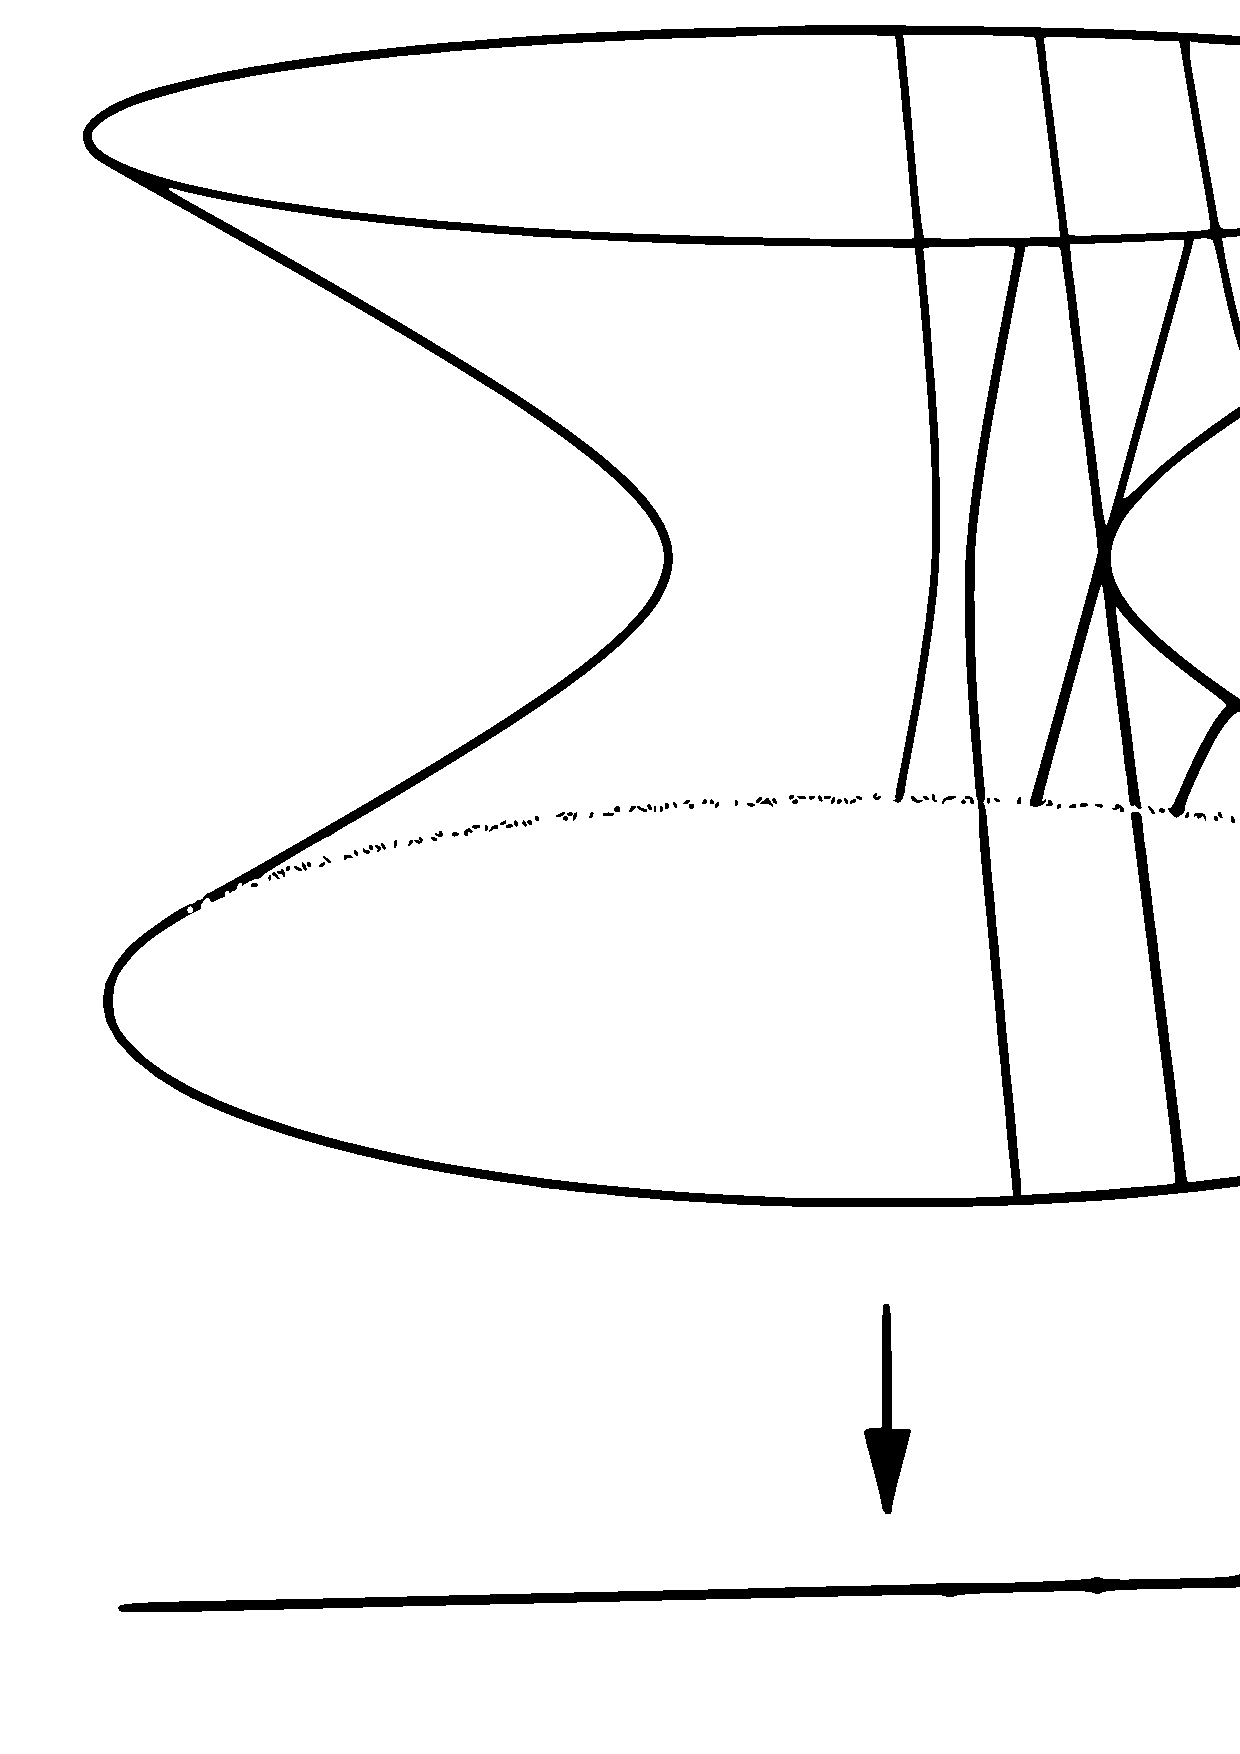
\includegraphics[scale=0.5]{chap_2/pics/21.png}\end{wrapfigure}
\noindent\textbf{Exercise\hspace{0.38em}{\addtocounter{thm}{1}}\thethm.}(这题需要有一定的射影几何知识。)设$(p)\in\spec\zz$满足$p\neq 5$且$p\equiv 1\text{ mod } (4)$,则$X$在点$(p)$上的纤维是一个双曲线,即,它相交于纤维$\mathbb{A}_{\mathbb{F}_p}^2$中“无穷远直线”的两个点,此二点的剩余类域是$\mathbb{F}_p$以及同构于$\mathbb{A}_{\mathbb{F}_p}^1-\{0\}$. 举个例子,若$(p)$上的纤维是曲线$x^2+y^2-5=0$,则它在$\mathbb{F}_p$上的投射平面上的闭包具有方程$X^2+Y^2-5Z^2=0$,于是它在无穷远处交直线$Z=0$于两点$[1,\alpha,0]$,其中$\alpha^2=p-1\text{ mod } (p)$. 证明,与此不同,若$p\equiv 3\text{ mod } (4)$,则纤维是一个椭圆,即,它与无穷远直线相交于一个点,该点处的剩余类域是$\mathbb{F}_{p^2}$. \vspace{0.5em}

上述图像非常符合其几何类比,一个纤维于一条曲线的曲面。比如,曲面$V(x^2-y^2-z)\subset \spec K[x$, $y$, $z]$纤维于$z$\hyp 直线$\spec K[z]$。纤维于一条曲线的曲面将具有有限个奇异纤维,正如右边的经典图片所示。

\subsection{$\mathbb{A}_\zz^1$中的双重点}

接着,我们考虑$\zz$上的双重点。再次,令
\[
	X=\bba_\zz^2=\spec\zz[x].
\]
若$Z\subset X$是一个支集只有一点的闭子概形,关联于素理想$(p,f)$,正如在域上的有限子概形那般,我们希望谈论$Z$的度。在域上的概形中,我们定义度为$\oo_Z(Z)$作为$K$\hyp 矢量空间的维度。但是现在$\oo_Z(Z)$可能不再能包含任意的域,比如它可能是$\zz/(p^2)$. 更加令人困惑的时候,它的剩余类域可能不是$\zz/(p)$. 因此,摆脱手头这困境最实惠的方式是,首先注意到基数$\# \oo_Z(Z)$一定具有形式$p^d$,进而可以我们可以取度为$d$,显然,如果$\oo_Z(Z)$是一个$\zz/(p)$\hyp 矢量空间的话,这就是它的维度。(一个更精致的方法是,先定义约态闭点的度为$\zz/(p)$\hyp 矢量空间的维度,然后定义$Z$的度为约态点的度乘以$Z$在该点的重数。)

比如考虑支集为点$(7,x)$的度为$2$的子概形,它们表现得很像域上的仿射平面上度为$2$的子概形。这样的子概形的理学一定包含极大理想$\pp=(7,x)$的平方,以及同样由$\pp^2$与一个$\pp$中的元素生成,因此
\[
	I=I_{\alpha,\beta}=(49,7x,x^2,\alpha 7+\beta x),
\]
其中$\alpha$, $\beta\in\zz$但不能同时被$7$整除。它只依赖于$\alpha$, $\beta$在$\zz/(7)$中的同余类,同时,将$(\alpha,\beta)$同时呈上$\zz/(7)$中的一个单位将不改变$I$. 因此,对每一个$7$元素域上的投射直线上的点$[\alpha,\beta]$,我们得到了一个支集为$\pp$的双重点。

\begin{exe}
证明这个对应是双射。
\end{exe}

支集为$(7,x)$的度为$2$的子概形的集合于是可以等同于域$K=\mathbb{F}_7$上的投射直线$\mathbb{P}_K^1$,就像域$K$上的$\mathbb{A}_K^2$的子概形可以等同于那个域上的投射直线。(在上述任何一种情况下的等同实际上都是将\textit{Zariski切空间}投射到外围空间中。\nottran)然而这有一个不同:$\mathbb{A}_K^2$中所有支集只有一点的度为$2$的子概形都是同构的,但是由$I_{\alpha,\beta}$定义的子概形$Z_{\alpha,\beta}$看起来是不同,甚至抽象地就可以看出来。若$\beta\neq 0$,我们有
\[
	Z_{\alpha,\beta}=\spec \zz/(49),
\]
但
\[
	Z_{1,0}=\spec(\zz/(7))[x]/(x^2)
\]
与其是不同构的。

\begin{exe}
分类,(a) 支集为点$(7,x)\in\mathbb{A}_\zz^1$的度为$3$的子概形,以及(b) 支集为点$(2,x^2+x+1)$的度为$4$的子概形。
\end{exe}

\begin{exe}\label{e.2.44}
参照第\pageref{p.2.18}页的图,使用前面的讨论来证明曲线$(4x + 1)$和$(x-2)$相切,而曲线$(4x + 1)$和$(11)$横截。
\end{exe}

最后,这里有一个$\spec \zz$上的平坦族的例子。回忆在上一节中讨论过直线对的族$M\cup L_t$,其中$M$是直线$x=z=0$以及$L_t$是直线$y=z-t=0$. 那里关键的观察是概形$M\cup L_t$的平坦族当$t\to 0$时并不是概形$M\cup L_0$,而是在原点有一个嵌入点的概形。

这里在由$\spec \zz$参数化的族也有着类似的现象。令$U=\spec \zz[7^{-1}]=\spec \zz-\{(7)\}$是点$(7)\in\spec\zz$的补,令
\[
	W=\bba_U^3:=\spec \zz[7^{-1},x,y,z]\subset \bba_\zz^2
\]
是对应的$\bba_\zz^3$的子概形。令$\mathscr{N}$与$\mathscr{L}$是$\bba_\zz^3$中由分别理想$(x,z)$以及$(y,z-7)$给出的闭子概形,再令$\mathscr{N}^*=\mathscr{N}\cap W$以及$\mathscr{L}^*=\mathscr{L}\cap W$. 令$\mathscr{X}^*$是$\mathscr{N}^*$和$\mathscr{L}^*$的并,$\mathscr{X}\subset \bba_\zz^3$是$\bba_\zz^3$中$\mathscr{X}^*$的闭包。于是,我们能把$\mathscr{X}^*$想成由$U$参数化的直线对的族,以及$\mathscr{X}$在点$(7)\in\spec \zz$的纤维$X_7$是这个平坦族“当$7$趋向于$0$”时的极限。正如我们期待的,纤维$X_7$的支集是$\mathscr{N}$与$\mathscr{L}$在点$(7)$处的纤维$(x=z=0)$与$(y=z=0)$的并,但概形$X_7$是非约态的,就像上一节的图片一样,它在原点处有一个嵌入点。

\begin{exe}
验证$\spec\zz$上$\mathscr{X}$的平坦性并描述$X_7$. 你能在$\spec\zz$上找到上节中讨论的其他平坦族的类似物吗?
\end{exe}
	% \def\PICDIR{chap_3/pics}

\chapter{射影概形}\label{chap:3}
\ThisULCornerWallPaper{1}{Pictures/3.png}

在我们理解了仿射概形后,射影概形\index{射影!概形}的理论并不会包含太多新奇的东西:在大多数情况下,它与射影簇的经典理论的差别完全类似于仿射概形和仿射簇的经典理论之间的差别。

我们首先将引入两个有限性条件,\textit{有限}以及\textit{有限型},然后定义和讨论\textit{分离}以及\textit{逆紧}态射\index{逆紧!态射},它们分别对应于绝大多数几何中的Hausdorff性与紧性。而正是部分因为射影簇和概形有这些性质,它们才是经典代数几何以及概形理论的基本研究对象。

这章的下一部分将引入射影概形以及给出一些例子。如同仿射概形的情形,有两种入手射影概形的法子:一种是定义出射影空间然后取它们的子概形,另一种是将所有的射影概形建立在同一个根基上,从分次代数入手。正如处理仿射情况那般,这里我们采用第二种方法。

在介绍了射影概形的基础定义以及它们的子概形后,我们将描述射影概形之间的态射,相较于仿射对应,它将更加微妙而难以捉摸(就像在簇范畴中那样)。我们将用一些射影概形的例子结束这节,其中最值得注意的是Grassmannian.

本章的最后一节将给出嵌入在射影空间中的射影概形的三个不变量,它们由 David Hilbert 所引入:Hilbert 多项式、Hilbert 函数以及自由分解(free resolution). 使用它们,我们有时能区分类似的概形,比如射影双重直线,以及可以
揭示平坦性的一些新现象。在一个射影概形的不变量中,可以根据其 Hilbert 多项式定义的不变量的是它的度数;在这方面的联系,我们将讨论著名的 B\'{e}zout 定理。

\section{一些态射的性质}\label{s:3.1}

\subsection{有限性条件}\label{s:3.1.1}

在大多数有关概形的非平凡结论中,有两个有限性条件。它们有着相似的名字但非常不同的性质。第一个有限性条件,有限型,是一个在绝大多数几何背景中产生的态射都满足的直截了当的性质,他被引入常是为了排除无穷维的纤维或者“非几何”的概形,比如局部环的谱。而另一个有限性条件,有限,比较起来就是一个非常严格的条件:它是说一个态射是逆紧的以及它的所有纤维都是有限的(特别地,零维的)。

首先,我们称一个概形间的态射$\varphi:X\to Y$是\textit{有限型}的,如果对每一点$y\in Y$,都存在一个$y$的仿射开邻域$V=\spec B\subset Y$使得它的原像被一族仿射开集$U_i\cong \spec A_i$有限覆盖,即
\[
	\varphi^{-1}(V)=\bigcup_{i=1}^n U_i,
\]
并且在映射
\[
	\varphi_V^\#:B=\oo_Y(V)\to \oo_X (\varphi^{-1}V)\to \oo_X(U_i)=A_i
\]
下,每个$A_i$都是一个有限生成$B$\hyp 代数。因此,比如,任意$\mathbb{A}_K^n$或$\mathbb{P}_K^n$的子概形是在$K$上有限型的(意思是,结构态射$X\to \spec K$是有限型的),而一个正维数的局部$K$\hyp 代数的谱不是。

一个态射$\varphi:X\to Y$被称为\textit{有限}\index{有限}的,如果对每点$y\in Y$都有它的一个开仿射邻域$V=\spec B\subset Y$使得原像$\varphi^{-1}(V)=\spec A$也是仿射的,以及通过拉回
\[
	\varphi_V^\#: B =\oo_Y(V)\to \oo_X(\varphi^{-1}V)=A,
\]
$A$是一个有限生成$B$-模。这是一个比有限型更强的条件,首先,马上可以由其给出$\varphi$的纤维是有限的,其次,拓扑空间之间的映射$|\varphi|:|X|\to |Y|$是一个闭映射。因此,对$Y=\spec B$以及多项式$f\in B[x]$,如果$f$的最高项系数是一个可逆元但其他不是,则态射$\spec(B[x]/(f))\to Y$是有限的。这些都可以参考 Eisenbud [1995, Chapter 4 and Section 9.1].

\subsection{逆紧性和分离性}\label{s:3.1.2}

许多几何技术当应用于紧Hausdorff空间时可以获得最完整的结果。尽管仿射概形在Zariski拓扑下是预紧的,但是它们并不共享在其他理论中紧空间的良好属性,因为Zariski拓扑不是Hausdorff的。举个例子,即使$X$是预紧的,仿射概形间的正则映射$\varphi:X\to Y$的像也可能不是闭的。

Zariski拓扑并不Hausdorff这点还有着其他令人不爽的结果。回忆在流形的一般定义中,我们从一个Hausdorff空间开始,在它上面装备一个坐标卡的覆盖,坐标卡是一个标准型(即欧式空间中的球)。但注意到,即使这些球都是Hausdorff的,也不足以说明整个空间是Hausdorff的。这就是为什么在Exercise \ref{exe:1.44} 中描述的具有双重原点的直线(这里重新展示如下)

\begin{center}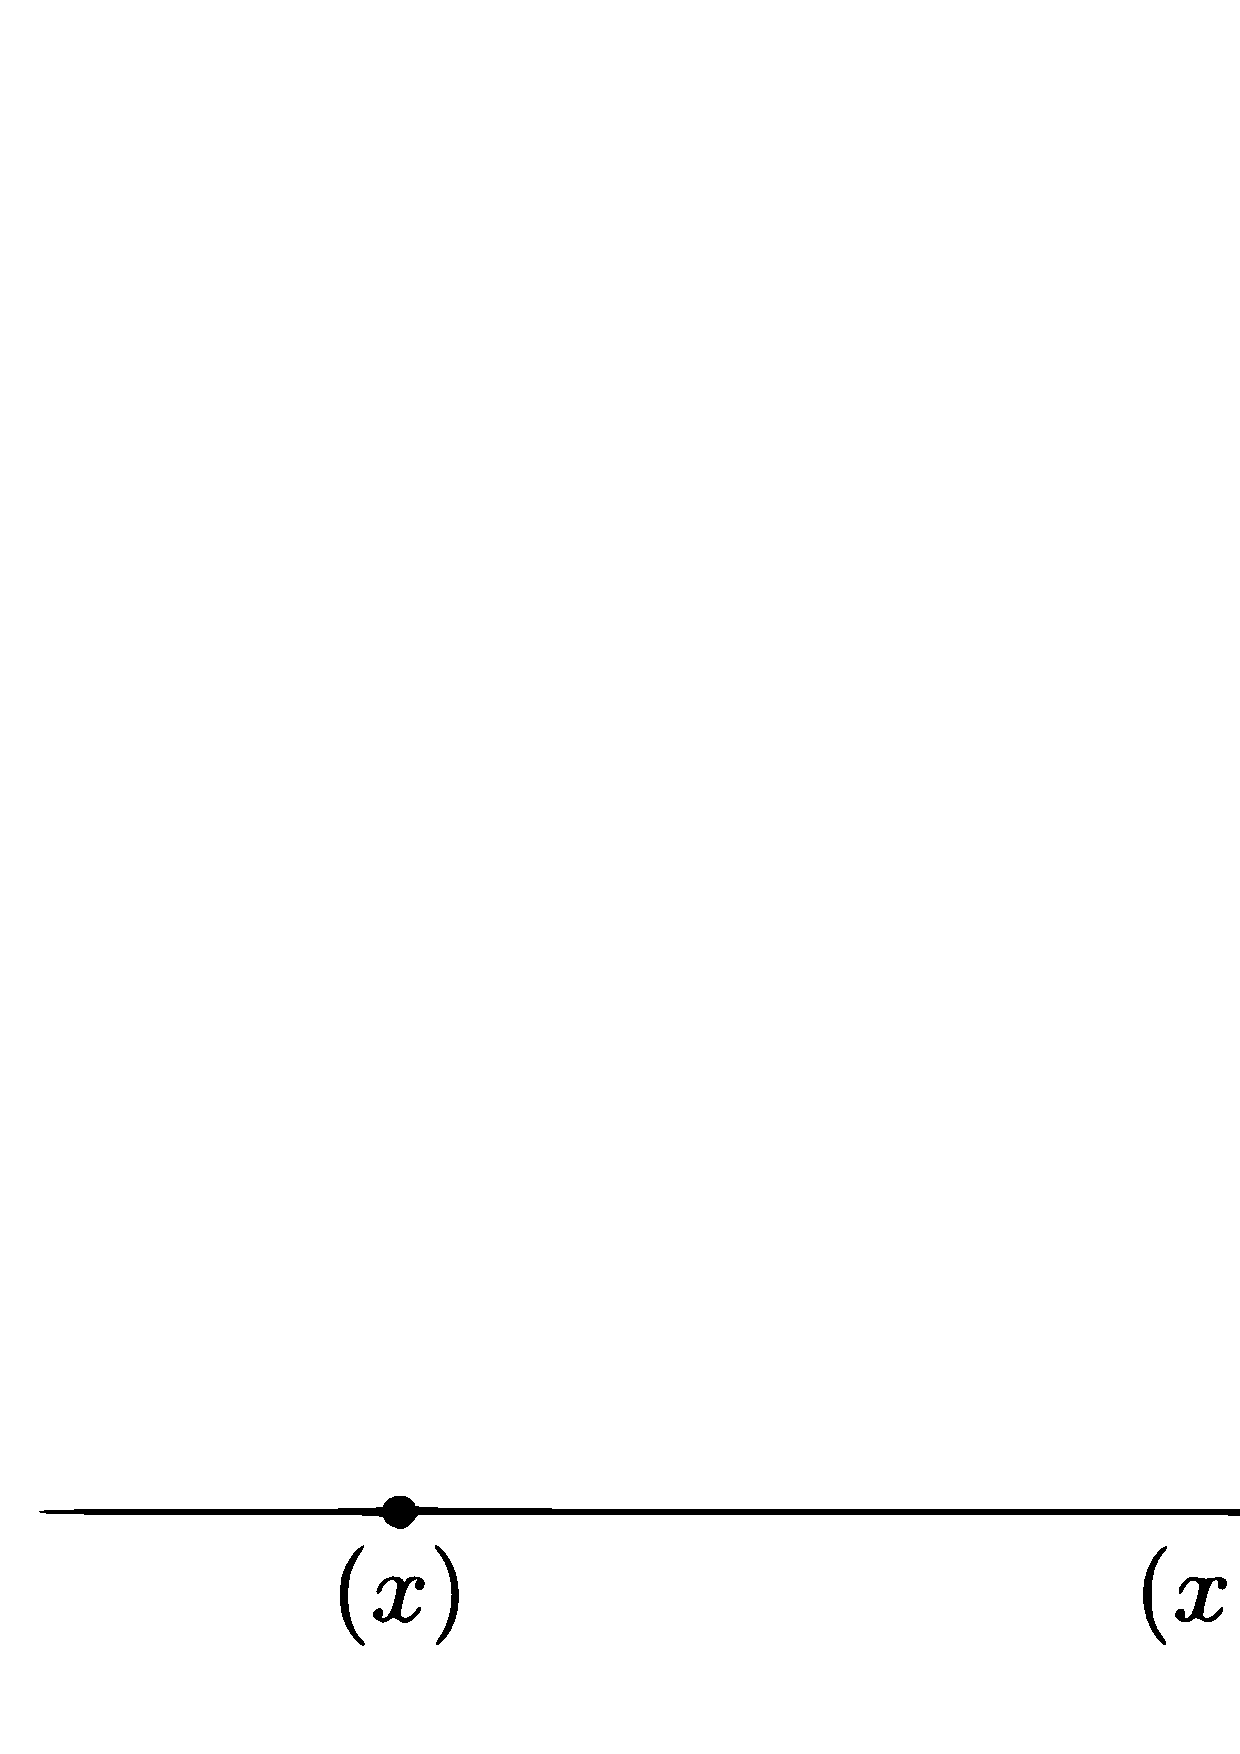
\includegraphics[scale=\scale,bb=0 0 562 68]{\PICDIR/1.png}\end{center}

\vspace{-0.4em}\noindent 不是一个流形。然而,在处理由仿射概形拼成的概形(或者簇)的时候,我们不能指定整个空间是Hausdorff的,因为即使就局部来说,那些拼合部件也不是Hausdorff的。于是,对给定两个概形之间的两个态射$\varphi$, $\psi:X\to Y$,$\varphi$和$\psi$相等的点构成的集可能不会是闭的。下面的习题是这方面的一个典型例子。

\begin{exe}
\begin{compactenum}[(a)]
\item 令$Y$是在域$K$上的具有双重原点的直线,正如在Exercise \ref{exe:1.44} 中的定义,以及令$\varphi_1$, $\varphi_2:\mathbb{A}_K^1\to Y$是两个显然的含入映射,证明$\varphi_1$和$\varphi_2$相等的点(仅作为拓扑空间间的连续映射)构成的集合不是闭的。
\item 现在令$X=Y\times_K Y$以及$\varphi$和$\psi$分别是两个到$X$到$Y$的典范投射。证明,$\varphi$和$\psi$相等的点构成的集合不是闭的(注意到这就是下面要定义的对角线)。证明,使得$\varphi$和$\psi$相等的闭点构成的集合也不是闭的。所以,这个病态现象并不是概形特有的,它在簇范畴中已经出现了。
\end{compactenum}
\end{exe}

然而,当$X$是一个仿射概形时,这样的病态现象并不会出现,同样,当$X$是一个射影概形时,这样的事情也被证明是不会出现的。这些概形所具有的理想性质,正是对应的流形上Hausdorff性的最重要结果之一(分离性),它表为:$X$作为一个概形在$K$上是\textit{分离的}。一般地,给定概形间的任意的映射$\alpha:X\to S$,我们定义\textit{对角}子概形$\Delta\subset X\times_S X$如下:局部地,在$X\times_S X$的每一个仿射开集上
\[
	X\supset \spec A\xrightarrow{\alpha|_{\spec A}}\spec B\subset S,
\]
它由所有形如
\[
a\otimes 1 - 1\otimes a \in A\otimes_B A
\]
的元素生成的理想$I$所定义。接着,我们称$\alpha$是\textit{分离的},或者说$X$是\textit{在$S$上分离的概形},如果$\Delta$是$X\times_S X$的一个闭子概形。

\begin{exe}
令$Y\to S$是拓扑空间之间的一个映射,然后令
\[
	\Delta \subset Y\times_S Y
\]
是其对角。证明,如果$\Delta$是一个闭集,那么对任意的交换图
\[
	\xymatrix{
		X\ar@<0.3ex>[rr]^\varphi \ar@<-0.3ex>[rr]_\psi\ar[dr] &&Y\ar[ld]\\
		&S&
	}
\]
$X$中使得$\varphi$和$\psi$相等的点集是一个闭集。现在证明对概形正则映射的相似引理:证明,存在一个自然定义的(即,极大的)闭子概形使得限制在上面$\varphi$和$\psi$是相同的。
\end{exe}

\begin{exe}
	令$X$是一个在$S$上分离的概形。证明$X$的(闭或开)子概形依然在$S$上分离。
\end{exe}

\begin{exe}
	注意,从对角子概形的定义来看,仿射态射是分离的。
\end{exe}

我们在下面将看到射影概形(等等就会定义)同样是分离的,因此,至少这些Hausdorff空间的性质对它们也是成立的。

在经典的仿射簇的情形中(即使简单如平面曲线),在上个世纪初就意识到,得到一些表现得像一个紧的对象的东西(实际上,在复数域上的仿射簇的情形中,在通常的拓扑下就是紧的),最简单的方式是取一个仿射簇在射影空间中的闭包。事实证明,如果$\varphi:X\to Y$是一个射影簇之间的映射,那么$\varphi$确实会将$X$的闭子簇映成$Y$的闭子簇。稍一般些,如果我们取这样一个映射以及一个任意的簇$Z$,得到
\[
	\psi:=\varphi\times 1_Z:X\times Z\to Y\times Z,
\]
则$\psi$将$X\times Z$的闭子簇映到$Y\times Z$的闭子簇。事实证明,\textit{这个性质连同分离性是使得射影概形如此有用的核心性质}。但是,满足这性质的簇要比射影簇稍多,而且它有时比起射影性更容易验证,所以给一个更一般的定义很重要。

如果$\alpha:X\to S$是一个概形之间的有限型映射,如果$\alpha$是可分的且对所有的映射$T\to S$,纤维积的投影
\[
	X\times_S T\to T
\]
将闭子集变成闭子集,则称$\alpha$是\textit{逆紧的},或者说$X$\textit{在$S$上逆紧}。同前,如果$S=\spec R$是一个环,我们时常会说“在$R$上逆紧”来意指“在$\spec R$上逆紧”。

上面对$\alpha$在分离性外给出的条件时常被叫做$\alpha$是\textit{全景闭的}。\textit{逆紧}这个名字来自一个旧的几何概念:一个Hausdorff空间之间的映射$\alpha:M\to N$被称为逆紧的如果每一个紧集的原像都是紧的。这是映射$\alpha$的一种相对紧性。这个性质与我们的定义之间的联系见下面的习题。

\begin{exe}
令$\mathscr C$是具有可数拓扑基的局部紧Hausdorff空间构成的范畴。证明映射$f:X\to Y$在$\mathscr C$中是全景闭的当且仅当他是逆紧的,即对任意的$Y$中的紧集$C$,$f^{-1}(C)$也是紧的。
\end{exe}

不管对于概形还是对于簇,逆紧这个概念已被证明是代数几何中的关键性质,它起到了其他几何理论中“紧且Hausdorff”的作用。下面我们将引入的射影概形是最一般的在给定概形$B$上逆紧的概形的例子。我们这里不会证明这个关键的结论,它并不是很难,但是将把我们引开太远。证明可以参见,比如,Hartshrone [1977, Theorem II.4.9].

一个有限态射$\varphi:X\to Y$当然是逆紧的,见Eisenbud [1995, Section 4.4].

\section{分次环的\texorpdfstring{$\proj$}{Proj}}\label{s:3.2}

\subsection{\texorpdfstring{$\proj S$}{Proj S}的构造}\label{s:3.2.1}

到目前为止,非仿射概形最重要的例子是在仿射概形$\spec A$上的\textit{射影}概形,
其中$A$是任意一个交换环。(为简单起见,我们常常说一个概形在$A$上射影,
而不说在$\spec A$上射影。)这样的一个概形来自于一个分次$A$-代数,而构造过程
非常类似于从它的齐次坐标环构造一个射影簇。我们同样可以从一个分次$\oo_B$-代数层
开始,定义在任意的基概形$\spec B$上射影的概形,这个推广有重要的应用。
但对这个理论中的大部分情况而言,我们都可以将情况约化到$B$是一个仿射概形,
故而在这里,我们对一般性的追求也仅止于此。

为了描述这个构造,我们从一个正分次$A$-代数开始,其中$A$是这个代数的$0$次部分,
即一个$A$-代数$S$具有分次
\[
	S=\bigoplus_{\nu=0}^\infty S_\nu\quad \text{(作为$A$-模)}
\]
使得
\[
	S_\nu S_\mu \subset S_{\nu+\mu}\quad \text{以及} \quad S_0=A.
\]
$S$中的一个元素如果处于$S_\nu$中,则它被称为$\nu$-\textit{次齐次}的。我们
将从$S$定义一个$A$-概形$X=\proj S$. 在$A$上射影的概形就被定义为具有形式
$\proj S$的概形,其中$S$是一个有限生成$A$-代数。代数$S$被称为$X$的
\textit{齐次坐标环},尽管(类似于射影簇的齐次坐标环)实际上他并不由$X$所决定。

当$S$是$A$上的多项式环
\[
	S=A[\text{$x_0$, $\dots$, $x_r$}]
\]
时,它具有如下分次:$A$中的元素是零次的,而每一个变量的分次都是$1$,则给出的
概形$\proj S$被称为\textit{$A$上的射影$r$-空间},记作$\mathbb{P}_A^r$.
(后面的习题将说明这个概形与第 \ref{chap:1} 章中定义的概形$\mathbb{P}_A^r$
是相同的。)在$A=K$是一个域的例子中,概形$\mathbb P_K^r$与$K$上的
名为射影空间的簇之间的关系就类似于概形$\mathbb A_K^r$与名为仿射$r$-空间
的簇之间的关系。

简单起见,我们将假设代数$S$在$A$上被它的$1$-次元素所生成,类似于多项式环那样,
一般的情况我们留做习题。(换个推广方向,如果$S$并没有假设在$A$上有限生成,
下面我们说的绝大部分内容依然成立,但这种推广用得相对较少)。

$\proj S$可以如下定义:将$S$中的正次齐次元生成的理想记作
\[
	S_+=\bigoplus_{\mu=1}^\infty S_\mu.
\]
我们称一个理想是\textit{齐次}的如果它由齐次元所生成。底空间$|\proj S|$是环$S$中所有不包含$S_+$的齐次素理想的集合(它们有时候被叫做\textit{相关}素理想,而$S_+$因此被叫做\textit{无关理想})。$|\proj S|$上的拓扑通过闭集定义,闭集取做形如
\[
	V(I):=\{\pp\,|\,\text{$\pp$是$S$的包含$I$的相关素理想}\}
\]
的集合,其中$I$是$S$的齐次理想。

我们将在开集基的每一个元素上明确$|\proj S|$的概形结构。为此,令$f$是$S$
的任意$1$-次齐次元素,以及$U$是开集
\[
	|\proj S|-V(f),
\]
即所有不包含$f$的齐次素理想(于是也不包含$S_+$)。$U$中的点可以等同于
$S[f^{-1}]$中的齐次素理想。另一方面,这些齐次素理想对应于环$S[f^{-1}]$
中所有的$0$-次元素的环,记作$S[f^{-1}]_0$,的素理想;
见Exercise \ref{exe:3.6}(a). 
于是,我们可以将$U$与拓扑空间$\spec S[f^{-1}]_0$相等同,
然后给他一个相应的仿射概形结构。我们将用$(\proj S)_f$来记这些
$\proj S$的仿射开子概形。如果$1$-次元$x_0$, $x_1$, $\dots$们生成了一个理想,
它的根是无关理想$S_+$,于是开集
\[
	(\proj S)_{x_i}:=\proj S-V(x_i)
\]
就构成了$\proj S$的一个仿射开覆盖。

如果$g$是$S$的另一个$1$-次元,则重叠部分$(\proj S)_f\cap (\proj S)_g$
是$(\proj S)_f$的由
\[
	S[f^{-1}]_0[(g/f)^{-1}]=S[f^{-1},g^{-1}]_0
\]
的谱给出的仿射开集。因为上式关于$f$和$g$对称,所以我们有一个自然的等同
\[
	((\proj S)_f)_{(g/f)}=((\proj S)_g)_{(f/g)}.
\]
正如第 \ref{s:1.2.4} 节中讨论的黏合构造,它们将$\proj S$变为了一个概形。

在本节的剩余部分以及下节中,我们将展示一些射影概形的基本事实以及
它们的闭子概形。因为这些事实以及它们的证明与簇的情况中的很类似,
我们将它们留作习题。

% proofread @ 2018.04.01

\begin{exe}~\label{exe:3.6}
\begin{compactenum}[(a)]
\item 对$S$任意的齐次理想$I$,以及$1$-次齐次元$f$,交集
\[
	(I\cdot S[f^{-1}])\cap S[f^{-1}]_0
\]
由一族$I$的齐次生成元乘以合适的$f$的(负的)次幂生成
($f$是任意次的推广见 Exercise \ref{exe:3.10})。
于是,$S[f^{-1}]$的齐次素理想一一对应于$S[f^{-1}]$的$0$-次元构成的环的素理想。
对应由$S[f^{-1}]$的素理想$\pp$变为$\mathfrak q=\pp\cap S[f^{-1}]_0$给出,
其逆为将$S[f^{-1}]_0$的素理想$\mathfrak{q}$变为$\mathfrak qS[f^{-1}]$.

\item 令$S=A[x_0$, $\dots$, $x_r]$为多项式环,
而$U$是$\mathbb P_A^r=\proj S$的仿射开集$(\mathbb P_A^r)_{x_i}$. 由定义,
\[
	U=\spec S[x_i^{-1}]_0,
\]
证明
\[
	S[x_i^{-1}]_0=A[x'_0,\dots,x'_r]
\]
为生成元$x'_j=x_j/x_i$的多项式环。(
注意$x'_i=1$,所以这是一个$r$变量的多项式环。)于是
\[
	(\mathbb P^r_A)_{x_i}=\mathbb A_A^r
\]
所以射影$r$-空间被$r+1$个仿射$r$-空间所覆盖,
就像第 \ref{chap:1} 章中所描述的那样。

\item 考虑一个映射$\alpha:S\to S[x_i^{-1}]_0$,
他将$x_i$变为$1$以及对$j\neq i$将$x_j$变为$x'_j$. 
从(a)证明如果$I$是$S$的一个齐次理想,于是
\[
	I':=I\cdot S[x_i^{-1}]\cap S[x_i^{-1}]_0=\alpha(I)'\cdot S[x_i^{-1}]_0.
\]
从$I$构造$I'$的过程被称为\textit{非齐次化}。
像经典的那样,描述与其相反的过程,齐次化。
\end{compactenum}
\end{exe}

\begin{exe}\label{exe:3.7}
如果$I$是一个分次环$S$的齐次理想,我们有一个底空间的包含
\[
	|\proj S/I|\subset |\proj S|.
\]
证明,这个子集与一个仿射开集$(\proj S)_f$的交集是$(\proj S)_f$的一个闭子集,
所以$\proj S/I$能被看作$\proj S$的一个闭子概形。
每个由$1$-次元有限生成的$A$-代数是某个多项式环
$A[x_0$, $\dots$, $x_r]$模掉一个齐次理想得到的商环,
所以我们看到\textit{每个$A$上的射影概形是一个$A$上的射影空间的闭子概形}。
下面我们将在Exercise \ref{exe:3.15} 和 \ref{exe:3.16} 具体看到环$S$的理想
与$\proj S$的闭子概形之间的联系。
\end{exe}

\begin{exe}\label{exe:3.8}
证明$\mathbb P_A^r$是开集$\mathbb A_A^{r-1}$与闭集$\mathbb P_A^{r-1}$
的不交并。特别地,$\mathbb P^0_A=\spec A$. 所以比如,
我们能将$\mathbb P_{\mathbb Z}^1$看成$\zz$上的仿射直线$\mathbb A_\zz^r$
(如第 \ref{chap:2} 章的图)与一个同构于$\spec \zz$的“无穷远点”的并,
如下图所示

\inclugra{2.png}
\end{exe}

\begin{exe}\label{exe:3.9}
在上图中添入点$(4x_1-5x_0)$, $(2x_1-5x_0)$以及$(5)$的闭包
(可以与第 \ref{s:2.4.3} 节中的$\mathbb A_{\mathbb Z}^2$的图相比较)。
\textit{注意}:曲线$(4x_1-5x_0)$应该画得与“无穷远点”$(x_0)$相切,
而曲线$(2x-5x_0)$不能。通俗地,我们可以说这是因为函数$5/4$在$(2)$
处有一个双极点,而$5/2$只有一个单极点。
(同样可见 Exercise \ref{exe:2.38} 中的讨论。)
\end{exe}

\begin{exe}\label{exe:3.10}
按上面的记号,令$h$为$S$的一个正次齐次元。集合
\[
	(\proj S)_h:=\proj S-V(h)
\]
同前为$S$中不包含$h$的齐次素理想构成的集合。
证明这个集合依然一一对应于$S[h^{-1}]_0$的素理想,
所以实际上存在一个$\spec S[h^{-1}]_0$与$\proj S$的(仿射)开子概形的同构。同样证明,这样的仿射开集族
\[
	\{(\proj S)_h\}_{h\in H}
\]
是一个$\proj S$的开覆盖,当且仅当$H$的元素生成了一个根为$S_+$的理想。
\end{exe}

\begin{exe}\label{exe:3.11}
推广$\proj S$的定义到$S$不被$1$-次元所生成的情况,以及证明$\proj S$是一个射影概形。
\end{exe}

\begin{exe}\label{exe:3.12}
令$S$是一个分次环,没必要是有$1$-次元生成的。
对任意的正次$d$,定义$S$的$d$-次\textit{Veronese 子环}为分次环
\[
	S^{(d)}=\bigoplus_{\nu=1}^\infty S_{d\nu}
\]
证明$\proj S$同构于$\proj S^{(d)}$. 
然而,证明如果$S=A[x,y]$,则$S^{(d)}$作为分次代数(甚至仅作为环)并不同构于$S$. 
于是,就像在簇中那样,分次代数与射影概形的对应并不是一一的。
\end{exe}

\subsection{\texorpdfstring{$\proj R$}{Proj R}的闭子概形}\label{s:3.2.2}

一个齐次理想$I\subset A[x_0$, $\dots$, $x_r]$确定了一个凝聚理想层$\tilde I\subset \mathscr O_{\mathbb P_A^r}$,因而一个$\mathbb P_A^r$的闭子概形。下面的习题建立了这些事实。

\begin{exe}\label{exe:3.13}
对每个开集
\[
	U_i=(\mathbb P_A^r)_{x_i}=\spec A[x_0,\dots,x_r,x_i^{-1}]_0\cong \mathbb A_A^r,
\]
令$\tilde I(U_i)$为理想$I\cdot A[x_0,\dots,x_r,x_i^{-1}]\cap A[x_0,\dots,x_r,x_i^{-1}]_0$. 证明这个定义可以以唯一的方式扩张到其他开集$U$上使得$\tilde{I}$成为一个凝聚理想层。所以我们称$\mathbb P_A^r$的闭子概形$V(\tilde{I})$\textit{关联于一个齐次理想$I$}.
\end{exe}

\begin{exe}\label{exe:3.14}
反之,给定一个$\mathbb P_A^r$的一个闭子概形,我们可以定义一个齐次理想$I(X)\subset A[x_0$, $\dots$, $x_r]$,它是齐次多项式$p(x_0,\dots,x_r)$生成的理想,其中齐次多项式需满足对每一个$i$,将其置于$1$后给出了元素
\[
	p(x_0,\dots,1,\dots,x_r)\in \mathscr I_X(U_i)\subset A[x_0,\dots,x_r,x_i^{-1}]_0.
\]
证明,如果$I=I(X)$,则$\tilde I=\mathscr I_X$.
\end{exe}

注意到连同 Exercise \ref{exe:3.7} ,它说明了每一个射影簇的闭子概形也是射影的:如果$I\subset S=A[x_0$, $\dots$, $x_r]$是一个齐次理想,则$V(\tilde{I})\subset \mathbb P^r_A$同构于概形$\proj S/I$.

\begin{exe}\label{exe:3.15}
子概形与理想的对应不再像仿射概形的情况是一一对应了。比如,证明在$\mathbb P_K^1$中,其中$K$是一个域,理想$I=(x_0)$和$I'=(x_0^2,x_0x_1)$都定义了同一个既约、单点子概形。更一般地,证明,如果$I\subset S=K[x_1$, $\dots$, $x_r]$是任意的齐次理想,以及对任意的整数$n_0$,通过
\[
	I'=\bigoplus_{n\geq n_0}I_n
\]
定义一个理想$I'\subset I$,则$I$和$I'$定义了$\mathbb P_K^r$的同一个子概形。
\end{exe}

\begin{exe}\label{exe:3.16}
为了解决这点,定义一个齐次理想$J\subset S:=A[x_0$, $\dots$, $x_r]$的\textit{饱和化}为理想
\[
	I=\{F\in S\,:\, \text{对某个$n$,$F\cdot S_n\subset J$}\},
\]
以及,称一个齐次理想是\textit{饱和}的,如果它等于它的饱和化。证明,存在一个$\mathbb P_A^r$的子概形与饱和理想之间的一一对应。
\end{exe}

\begin{exe}\label{exe:3.17}
证明,Exercise \ref{exe:3.12} 中的同构定义了一个射影空间$\mathbb P_A^r$以及$\mathbb P_A^N$的一个闭子概形之间的同构,其中$N=\dim_A(A[x_0$, $\dots$, $x_r]_d)$.(这就是概形版的Veronese映射。)
\end{exe}

\begin{exe}\label{exe:3.18}
证明,如果$R$是一个环$A=R_0$上的有限生成分次环(没必要是由其$1$-次元生成的),$\proj R$同构于某个射影空间$\mathbb P_A^r$的闭子概形。
\end{exe}

我们以一个定义和基本定理结束这一小节。

\begin{defi}
一个概形间态射$\varphi:X\to Y$被称为\textit{射影}的,如果他是一个闭嵌入$X\to \mathbb P_Y^n$和结构态射$\mathbb P_Y^n\to Y$的复合。
\end{defi}

注意到,如果$Y=\spec A$是仿射的,这相当于说$X$具有形式$\proj S$,其中$S$是一个有限生成$A$-代数。射影态射的基本事实前面已经说过了:

\begin{thm}\label{thm:3.20}
射影态射是逆紧的。
\end{thm}

证明可见Hartshorne [1977, Theorem II.4.9].

\begin{exe}\label{exe:3.21}
证明,有限态射$\varphi:X\to Y$是逆紧的且局部射影的,所谓局部射影即指,
$Y$可以被开集族$U\subset Y$所覆盖,使得限制$\varphi:V=\varphi^{-1}U\to U$
是射影的。(我们采用了 Hartshorn [1977, Section II.4] 中射影态射的定义,
而在 Grothendieck [1961, EGA II, 5.5] 中,
射影是指我们这里被叫做局部射影的性质。)
\end{exe}

\subsection{整体\texorpdfstring{$\proj$}{Proj}} \label{s:3.2.3}

\paragraph*{分次\texorpdfstring{$\oo_X$}{OX}-代数层的\texorpdfstring{$\proj$}{Proj}}\addcontentsline{toc}{subsubsection}{分次\texorpdfstring{$\oo_X$}{OX}-代数层的\texorpdfstring{$\proj$}{Proj}}
分次环$S$的$\proj$的构造给出了一个概形$X=\proj S$以及一个结构态射
$X\to B=\spec(S_0)$. 因为$\proj S$与$S$的关联是函子性的,
所以存在一个更一般的构造,给出概形$X$以及结构态射$X\to B$,
其中$B$是任意概形,使得当$B$是仿射的时候将回到$\proj$:对一般的$B$,
我们只需用$\oo_B$上的代数层代替分次$S_0$-代数$S$.

为实现这个构造,令$B$为任意概形,一个\textit{拟凝聚分次$\oo_B$-代数层}
是指一个$B$上的拟凝聚代数层$\mathscr F$,具有一个分次
\[
	\mathscr F=\bigoplus_{\nu=0}^\infty \mathscr F_\nu
\]
使得$\mathscr F_\nu \mathscr F_\mu\subset \mathscr F_{\mu+\nu}$
以及$\mathscr F_0=\oo_B$. 因此,对每一个仿射开集$U\subset B$,
其坐标环为$A=\oo_B(U)$,环$\mathscr{F}(U)$是一个分次$A$-代数,
其$0$-次部分为$\mathscr F(U)_0=A$. 

给定这样一个层$\mathscr F$,对每个仿射开集$U\subset B$,
我们令$X_U\to U$为概形$X_U=\proj \mathscr F(U)$及结构态射
$\proj \mathscr F(U)\to \spec A=U$. 对每个$B$的开子集的含入$U\subset V$,
限制映射$\mathscr F(V)\to \mathscr F(U)$是一个分次环的同态,
其$0$-次部分为限制映射$\oo_B(V)\to \oo_B(U)$,
所以诱导了一个映射$X_U\to X_V$与结构态射$X_U\to U$和$X_V\to V$以及
含入$U\hookrightarrow V$可交换。我们于是可以将概形$X_U$粘起来得到概形
$X$,其具有结构态射$X\to B$,记作$\proj \mathscr F$,
而$X$的构造则被称为\textit{整体$\proj$}.

就像在普通的$\proj$中一样,大部分情况下代数层$\mathscr F$由其$1$-次部分$\mathscr F_1$所生成,以及$\mathscr F_1$是凝聚的(或者,某种程度上更一般地,对某个$d>0$,Veronese 子层
\[
	\mathscr F^{(d)}=\bigoplus_{\nu=0}^\infty \mathscr F_{d\nu}
\]
由$\mathscr F_{d\nu}$所生成,而$\mathscr F_{d\nu}$是凝聚的
)。在这个假设下,同样如同普通的$\proj$,态射$\proj \mathscr F\to B$是逆紧的。

整体$\proj$最简单的例子给了我们任意概形$S$上的射影空间的另一个构造。回忆在第 \ref{chap:1} 章,任意概形$S$上的射影空间是黏合构造而成的:如果$S$被仿射概形族$U_\alpha=\spec R_\alpha$所覆盖,我们定义射影空间$\mathbb P_S^n$为射影空间$\mathbb P_{U_\alpha}^n$的并,并通过$U_\alpha\cap U_\beta$上的恒等映射诱导的黏合映射粘起来。此外,我们也可以通过乘积来定义它:
\[
	\mathbb P_S^n=\mathbb P_{\mathbb Z}^n\times_{\spec \mathbb Z}S.
\]
最后,我们可以将其实现为$S$上秩为$n+1$的自由层的对称代数的整体$\proj$:

\begin{exe}\label{exe:3.22}
令$S$为任意概形。证明$S$上的射影空间$\mathbb P_S^n$可以由整体$\proj$构造:
\[
	\mathbb P_S^n=\proj \left(\operatorname{Sym}(\oo_S^{\oplus n+1})\right).
\]
\end{exe}

特别地,在纤维积外,我们可以通过整体$\proj$来实现给定概形$S$上的射影空间的乘积:如果我们记$\oo_{\mathbb P_S^r}[X_0$, $\dots$, $X_m]$为分次$\oo_{\mathbb P_S^n}$-代数层$\operatorname{Sym}\left(\oo_{\mathbb P_S^n}^{\oplus m+1}\right)$,则
\[
	\mathbb P^n_S\times_S \mathbb P^m_S=\proj \oo_{\mathbb P^n_S}[X_0,\dots,X_m].
\]
第三种方式是通过\textit{Segre嵌入}:

\begin{exe}\label{exe:3.23}
令$S$为任意概形。证明
\begin{align*}
\mathbb P_S\times_S \mathbb P_S^m &\cong V\left(\{X_{i,j}X_{k,l}-X_{i,l}X_{k,j}\}\right)\subset \proj \oo_S[\{X_{i,j}\}_{0\leq i\leq n;0\leq j\leq m}]\\
& = \mathbb P_S^{(n+1)(m+1)-1}.
\end{align*}
\end{exe}

于是,至少局部地在基上,这给了我们一种方式来描述这样乘积的子概形:

\begin{exe}\label{exe:3.24}
令$S=\spec R$为任意的仿射概形。证明
\[
	X\subset \proj R[x_0,\dots,x_n]\times_S \proj R[y_0,\dots,y_m]=\mathbb P^n_S\times_S\mathbb P^m_S
\]
任意的闭子概形都可以由族$\{F_\alpha(x_0$, $\dots$, $x_n;y_0$, $\dots$, $y_m)\}$的零点集给出,其中$F_{\alpha}$是两族变量$(x_0$, $\dots$, $x_n)$和$(y_0$, $\dots$, $y_m)$的齐次函数。特别地,证明矩阵
$
\begin{pmatrix}
x_0&x_1&\cdots &x_n\\
y_0&y_1&\cdots &y_n\\
\end{pmatrix}
$
的$2\times 2$子式的理想定义了$\mathbb P^n_S\times_S\mathbb P^m_S$中的对角集。推出任意射影态射都是可分的。
\end{exe}

整体$\proj$构造的一个更严肃的应用是定义概形$X$沿着闭子概形$Y\subset X$的\textit{爆破},我们将在第 \ref{chap:5} 章中完整地讨论它。整体$\proj$另一个通常的应用是我们下面描述的向量丛的射影化。

\paragraph*{凝聚层\texorpdfstring{$\mathscr E$}{E}的射影化\texorpdfstring{$\mathbb P(\mathscr E)$}{P(E)}}\addcontentsline{toc}{subsubsection}{凝聚层\texorpdfstring{$\mathscr E$}{E}的射影化\texorpdfstring{$\mathbb P(\mathscr E)$}{P(E)}}
在 Exercise \ref{exe:3.22} 中看到,概形$S$上的射影空间$\mathbb P_S^n$是$\proj(\operatorname{Sym}(\oo_S^{\oplus n+1}))$. 我们将对任意凝聚层$\mathscr E$做一个类似的构造,定义$\mathscr E$的\textit{射影化}$\mathbb P(\mathscr E)$为$B$-概形
\[
	\mathbb P(\mathscr E)=\proj(\operatorname{Sym} \mathscr E)\to B.
\]

检查最简单的情况,令$V$是域$K$上的$n$-维向量空间,看成单点概形$\spec K$上的一个向量丛。$V$的射影化是一个$K$上的维数为$n$的射影空间,而$V^*$的射影化被称为$\mathbb PV$的\textit{对偶射影空间}。$\mathbb P(V)$的$K$-值点对应于$V$的一维商空间,或者等价地,$V$中的超平面。$\mathbb P(V^*)$的$K$-值点对应于$V$的一维子空间,这就是被经典地记作$\mathbb P^n$的射影空间。

一般些,如果$\mathscr E$是一个秩为$n+1$的局部自由层,则$\mathbb P(\mathscr E)$为$B$上的一个\textit{射影丛},即对足够小的仿射开集$U\subset B$,$U$在$\mathbb P(\mathscr E)$中的原像作为$U$-概形同构于射影空间$\mathbb P_U^r$. (如果$\mathscr E$不是局部自由的,则概形$\mathbb P(\mathscr E)$是怎么样的就没那么清楚了。)当$B$是一个代数闭域$K$上的簇,而$\mathscr E$是一个$B$上的向量丛$E$的截面层,则$\mathbb P(\mathscr E^*)$的$K$-值点对应于$\mathscr E$的纤维的一维子空间,而$\mathbb P(\mathscr E)$的$K$-值点对应于$\mathscr E$的纤维的一维商空间,或等价地,纤维中的超平面。

注意到,任意闭子概形$X\subset \mathbb P_B^n$能被实现为$\proj(\mathscr F)$,其中$\mathscr F$是一个分次$\oo_B$-代数的拟凝聚理想层。更一般地,如果$\mathscr E$是任意凝聚层,则其射影化的任意闭子概形$X\subset \mathbb P(\mathscr E)$也可以如此实现。反之,如果$\mathscr F$是分次$\oo_B$-代数的任意拟凝聚理想层,由$\mathscr F_1$生成,则满射$\operatorname{Sym}(\mathscr F_1)\to \mathscr F$给出了嵌入$X=\proj \mathscr F\hookrightarrow \mathbb P(\mathscr F_1)$.

\begin{exe}\label{exe:3.25}
	令$K$是一个域,$\mathbb P_K^2=\proj K[X,Y,Z]$是$K$上的射影平面,$(\mathbb P_K^2)^*=\proj K[A,B,C]$是对偶射影平面。令$\Sigma$是$(\mathbb P_K^2)^*$上的万有直线,即
	\[
		\Sigma=V(AX+BY+CZ)\subset \mathbb P_K^2\times_K (\mathbb P_K^2)^*
	\]
	看作$(\mathbb P_K^2)^*$上的族。证明,$\Sigma\to (\mathbb P_K^2)^*$是$(\mathbb P_K^2)^*$上的秩为$2$的局部自由层$\mathscr E$,并描述$\mathscr E$.
\end{exe}

\begin{exe}\label{exe:3.26}
	令$B$是任意概形,$\mathscr E$是一个$B$上的局部自由层,以及$E=\spec (\operatorname{Sym}\mathscr E^*)\to B$是$\mathscr E$对应的向量丛的全空间。证明,我们可以将$E\to B$完备为一个$B$上的射影空间的从:确切地,证明,我们有一个$E$上的含入,到$\mathbb P(\mathscr E^*\oplus \oo_B)$作为其开子概形,补是一个超平面丛$\mathbb P(\mathscr E^*)\subset \mathbb P(\mathscr E^*\oplus \oo_B)$.
\end{exe}


\subsection{切空间和切锥} \label{s:3.2.4}
\paragraph*{仿射与射影切空间}\addcontentsline{toc}{subsubsection}{仿射与射影切空间}
概形的Zariski切空间是抽象向量空间,但当一个域$K$上的概形$X$被嵌入到一个背景空间中,比如仿射或射影$K$-空间,我们可以将$X$的一个剩余类域为$K$的点$p$关联于一个对应仿射或者射影空间的线性子簇,其被称为$X$在点$p$的\textit{仿射切空间}或\textit{射影切空间}。在仿射概形$X=V(f_1,\dots,f_k)\subset \mathbb A_K^n$以及点$p=(a_1,\dots,a_n)\in X$的情况中,这是一个由
\[
	V\left(\left\{
		\sum_i \frac{\partial f_\alpha}{\partial x_i}(\alpha_1,\dots,\alpha_n)\cdot (x_i-a_i)
	\right\}_{\alpha=1,\dots,k}
	\right)
\]
给出的子簇。为理解这个概形与Zariski切空间之间的关系,注意到域$K$上的一个向量空间与仿射空间$\mathbb A_K^n$并不是同一个东西。但是,给定$K$上的一个$n$-维向量空间$V$,我们可以对$V$给出一个概形$\overline{V}$,它同构于仿射开集$\mathbb A_K^n$,所以$\overline{V}$中剩余类域为$K$的点自然地对应于$V$中的向量:$\overline{V}$就是对偶空间对称代数的谱
\[
	\overline{V}=\spec (\operatorname{Sym}(V^*)).
\]
我们将称$\overline{V}$为\textit{对应于向量空间$V$的概形}。

这告诉我们,与域$K$上的仿射空间$\mathbb A_K^n$在$K$-有理点$p\in \mathbb A^n_K$(即一个剩余类域为$\kappa(p)=K$的闭点)的Zariski切空间相对应的概形$\overline{T_p(\mathbb A^n_K)}$,可以自然等同于仿射空间本身,它将$T_p(\mathbb A_K^b)$的原点变成了$p$. 现在,假设$X\subset \mathbb A_K^n$是任意的子概形,$p\in X$是任意的$K$-有理点。含入$\iota:X\hookrightarrow \mathbb A_K^n$在点$p$处的微分$d\iota_p$将Zariski切空间$T_p(X)$表为一个向量子空间
\[
	d\iota_p:T_p(X)\hookrightarrow T_p(\mathbb A_K^n).
\]
我们取概形的诱导含入
\[
	\overline{d\iota_p}:\overline{T_p(X)}\hookrightarrow
	\overline{T_p(\mathbb A_K^n)}=\mathbb A_K^n
\]
复合上平移态射$t_p:\mathbb A^n_K\to \mathbb A^n_K$,它将原点映射为$p$,得到一个含入
\[
	t_p\cdot \overline{d\iota_p}:\overline{T_p(X)}\hookrightarrow
	\mathbb A_K^n \longrightarrow \mathbb A_K^n.
\]
这个含入的像是$\mathbb A_K^n$的一个仿射子空间,我们将其称为$X$在点$p$的\textit{仿射切空间}。再一次注意到,这是一个概形不是一个向量空间。

对射影概形$X\subset \mathbb P_K^n$的剩余类域为$K$的点$p$,我们可以类似地对应于一个线性子空间$\mathbb T_p(X)\subset \mathbb P_K^n$. 一种实现它的方式是找一个包含$p$的开子集$U\cong \mathbb A_K^n\subset \mathbb P^n_K$,然后取$X\cap U$在点$p$的仿射切空间在$\mathbb P_K^n$中的闭包。但,我们也有另一种更内蕴的方式。首先,我们记背景射影空间$\mathbb P_K^n$为对应于向量空间$V$的射影空间$\mathbb PV$,即是
\[
	\mathbb P_K^n=\proj S
\]
其中
\[
	S=\operatorname{Sym}V^*
\]
是$V$的对偶空间的对称代数。因此,$S_1=V$的$(k+1)$-维线性子空间对应于$\mathbb P_K^n$中的$k$-平面。我们令
\[
	I=I(X)\subset S
\]
为$X\subset \mathbb P_K^n$的齐次理想,以及令$\mm=\mm_p\subset S$为在点$p\in X$为零的齐次多项式构成的理想。令$J$是理想$I+\mm^2\subset S$的饱和化。我们定义$X$在点$p$的射影切空间$\mathbb T_p(X)$为$\mathbb P_K^n$的子空间
\[
	\mathbb T_p (X)=V(J\cap S_1)\subset \mathbb P^n_K.
\]
稍加解释:注意到$J$是$p$在$X$中的一阶邻域的理想,即为$X$与$p$的理想$\mm$的平方定义的“丰满点”$P\subset \mathbb P_K^n$的交。于是,射影切空间$\mathbb T_p(X)=V(J\cap S_1)$就是由这个一阶邻域$V(J)$张成的,即是包含$V(J)$的$\mathbb P_K^n$的最小线性子空间。

\begin{exe}\label{exe:3.27}
	证明这个定义与前面的一开始说的\naive 定义一致。
\end{exe}

因为射影概形$X$在$K$-有理点$p\in X$处的射影切空间$\mathbb T_p(X)$是一个背景射影空间$\mathbb PV$的一个线性子空间,具有形式$\mathbb T_p(X)=\mathbb PW$,其中$W$是一个商向量空间$V\to W\to 0$. 然后,我们可能问向量空间$W$与Zariski切空间$T_p(X)$之间具有什么联系。在第 \ref{s:6.2.1} 节中,我们将看到答案是一个正合列
\[
	0\longrightarrow K\longrightarrow W^* \longrightarrow T_p(X)\longrightarrow 0.
\]
更明确一些,如果$V\to U\to 0$是$V$的一个$1$-维商空间,对应于点$p\in X\subset \mathbb PV$,则满射$V\to U$可以经由满射$\varphi:W\to U$分解,进而我们有一个自然的等同
\[
	T_p(X)=\Hom(\operatorname{Ker}\varphi,U).
\]
无论如何,注意到我们都有一个$\mathbb T_p(X)$中经过$p$的直线的集合与$T_p(X)$中经过原点的直线的集合之间的自然等同。

\begin{exe}\label{exe:3.28}
	令$X=V(F)\subset \mathbb P_K^n$是$\mathbb P_K^n$中的超平面,由齐次多项式$F(Z_0,\dots,Z_n)$给出,再令$p=[a_0,\dots,a_n]\in X$是任意一个剩余类域为$K$的点。证明,射影切空间$\mathbb T_p(X)$就是零点集$V(L)\subset \mathbb P_K^n$,其中$L$是线性多项式
	\[
		L(Z_0,\dots,Z_n)=\sum_{k=1}^n\frac{\partial F}{\partial Z_i}(a_0,\dots,a_n)\cdot Z_k.
	\]
\end{exe}

\paragraph*{切锥}\addcontentsline{toc}{subsubsection}{切锥}
对概形$X$在点$p\in X$的切向表现的更准确描述是它的切锥。为定义它,令$X$为任意的概形,$p\in X$是一个点,$\mathscr O_{X,p}$是$X$在点$p$的局部环,以及$\mm=\mm_{X,p}\subset \mathscr O_{X,p}$是$\mathscr O_{X,p}$的极大理想。我们定义$X$在点$p$的\textit{切锥}$TC_p(X)$为概形
\[
	TC_p(X)=\spec \left(\bigoplus_{\alpha=0}^\infty \mm^\alpha/\mm^{\alpha+1}\right).
\]
这个构造的一些简单观察如下。首先,注意到分次环$B=\bigoplus (\mm^\alpha/\mm^{\alpha+1})$由它的$1$-次分次部分
\[
	B_1=\mm/\mm^2=(T_pX)^*
\]
所生成的,因此,$B$是环
\[
	A=\operatorname{Sym}((T_pX)^*)
\]
的商环。我们于是有了一个含入
\[
	TC_p(X)=\spec B\hookrightarrow \spec A=\overline{T_pX},
\]
或者说,$X$在点$p$的切锥自然地是$X$在点$p$的Zariski切空间$T_pX$对应的概形的子概形。

为给出一个更切实的切锥实现,假设$X$是一个域$K$上的仿射空间的子概形,即
\[
	X\subset \spec K[x_1,\dots,x_n],
\]
再令$I=I(X)\subset K[x_1,\dots,x_n]$是$X$的理想;进一步假设点$p\in X$是原点$(x_1,\dots,x_n)\in \mathbb A_K^n$. 对任意的多项式$f\in K[x_1,\dots,x_n]$,记
\[
	f(x_1,\dots,x_n)=f_m(x_1,\dots,x_n)+f_{m+1}(x_1,\dots,x_n)+\cdots,
\]
其中$f_l(x_1,\dots,x_n)$是$l$次齐次多项式以及$f_m\neq 0$;首个非零项$f_m(x_1,\dots,x_n)$被称为$f$的\textit{领头项}%
%\footnote{译者注:英文是leading term,大概也可以称为首项?好像不太合适}%
。于是,我们有如下诠释:

\begin{exe}\label{exe:3.29}
	证明切锥
	\[
		TC_p(X)\subset \overline{T_pX}\subset \overline{T_p(\mathbb A_K^n)}=\mathbb A_K^n
	\]
	是由所有多项式$f\in I$的领头项的零点集定义的子概形。
\end{exe}

回到一般的情况,注意到因为环$B=\bigoplus (\mm^\alpha/\mm^{\alpha+1})$是分次的,我们可以同样对$(X,p)$关联一个几何对象$\proj B$. 这是$X$在点$p$的Zariski切空间对应的射影空间$\mathbb P(T_p X)\cong \mathbb P^n_{\kappa(p)}$的一个子概形,称作在$X$在点$p$的\textit{射影切锥},记作$\mathbb PTC_p(X)$. 在许多情况中,处理作为射影概形以及比切锥少一维的射影切锥会更方便,但一般来说,他比切锥所包含的信息稍少一些(就像下面的Exercise \ref{exe:3.30} 将展示的,切锥$TC_p(X)$可能在原点有一个嵌入点,而射影切锥没有)。

尽管,射影空间一般的子概形的次数将在第 \ref{s:3.3.1} 节中才定义,我们将在这里提出一个可以由$X$在点$p$的射影切锥定义的概形不变量:定义$X$在点$p$的\textit{重数}为射影切锥$\mathbb PTC_p(X)\subset \mathbb P(T_p X)\cong \mathbb P^n_{\kappa(p)}$的次数。这个定义展现了另一个例子,告诉我们为何概形会在处理簇时自然出现且十分方便:在簇范畴我们依然可以定义切锥(是对应于我们的切锥的既约概形)以及射影切锥,但是它们在族中表现得并不好。

% p.108

有许多非既约切锥的例子。比方说,考虑方程$C_t=\spec K[x,y]/(y^2-tx^2-x^3)$定义的平面三次曲线族(即,我们令$B=\mathbb A^1_K=\spec K[t]$,然后取我们的族为$\mathscr C=V(y^2-tx^2-x^3)\subset \mathbb A_B^2\to B$)。对每一个$t$,曲线$C_t$可以由$t\mapsto (\lambda^2-t,\lambda^3-t\lambda)$定义的映射
\[
	\mathbb A_K^1=\spec K[\lambda]\longrightarrow \mathbb A_K^2=\spec K[x,y]
\]
的像参数地给出。对$t\neq 0$,这个曲线在原点有一个结点,两个点$\lambda =\pm \sqrt t$都映为原点,这在切锥$\mathbb T_{(0,0)}C_t=V(y^2-tx^2)$也有所反应,它是两条直线$y=\pm \sqrt t x$的并。当$t=0$,我们看到曲线的结点退化为了一个尖点,而切锥现在是双重直线$\mathbb T_{(0,0)}C_0=V(y^2)$.

更精妙的例子,考虑由
\[
	\nu_1:t\longmapsto (t^3,t^4,t^5)
\]
以及
\[
	\nu_1:t\longmapsto (t^3,t^5,t^7)
\]
给出的映射$v_i:\mathbb A_K^1\to \mathbb A_K^3$的像确定的曲线$C_1$, $C_2\subset \mathbb A_K^3$. 在每个例子中,令$p$是$C_i$的奇异点。

\begin{exe}~\label{exe:3.30}
	\begin{compactenum}[(a)]
		\item 证明,两条曲线的射影切锥
		\[
			\mathbb PTC_p(C_i)\subset \mathbb P_K^2
		\]
		是一个次数为$3$的曲线%
		\footnote{
			译者注:定义见Exercise \ref{exe:2.18}.
		}%
		概形,即,同构于$\spec K[s]/(s^3)$,以及它们不被包含于任何$\mathbb P_K^2$的直线中。
		\item 找一个例子,曲线$C\subset \mathbb A_K^3$在原点的射影切锥同构于$\spec K[s]/(s^3)$以及包含于一条直线中。
		\item 找一个例子,曲线$C\subset \mathbb A_K^3$在原点的射影切锥同构于$\spec K[s,t]/(s^2,st,t^2)$.
		\item 找一个例子,曲线$C\subset \mathbb A_K^3$在原点的射影切锥包含于一条直线中,但Zariski切空间$T_0(C)$却是三维的。
	\end{compactenum}
\end{exe}

对概形$X$在点$p\in X$的切锥有另一个几何的刻画:直接将切锥定义为,\textit{切锥是点$p$连同上直线$\overline{pq}$由点$q\neq p\in X$趋近点$p$的极限位置的轨迹。}为更准确地描述这个定义,首先假设$p\in X$的一个邻域被嵌入在$K$上的仿射空间$\mathbb A_K^n$中,令$T=\overline{T_p\mathbb A_K^n}$是$\mathbb A_K^n$在点$p$的Zariski切空间$T_p\mathbb A_K^n$对应的仿射空间,以及考虑关联对应
\[
	\Sigma = \left\{(v,q)\;:\;v\in \overline{T}_p(\overline{pq})\subset T\times (\mathbb A_K^n \setminus \{p\})\right\}.
\] % p.109
等价地,通过将$T$与$\mathbb A_K^n$本身等同起来,则$\Sigma$是$\mathbb A_K^n\times (\mathbb A_K^n \setminus \{p\})$的由方程
\[
	y_i\left(x_j-x_j(p)\right)-y_j\left(x_i-x_i(p)\right)=0
\]
给出的子概形。令$\Gamma=\pi_2^{-1}(X\setminus \{p\})\subset T\times (X\setminus \{p\})$是$X\setminus \{p\}$在$\Sigma$中的原像,$\overline{\Gamma}$是$\Gamma$在$T\times X$中的闭包。则我们有:

\begin{pro}\label{pro:3.31}
切锥$TC_p X$是$\overline{\Gamma}$在点$p\in X$处的纤维。
\end{pro}

这个命题(模掉$TC_p X$中在原点处可能的嵌入分支)将在第 \ref{chap:4} 章中证明。这个命题相当于说,$TC_p X$的射影化是$X$在点$p$的爆破的例外除子。

Proposition \ref{pro:3.31} 相当有用,比方说在做下面的Exercise \ref{exe:3.32}--\ref{exe:3.34} 的时候。

\begin{exe}\label{exe:3.32}
令$V$是$\mathbb P_K^1=\proj K[X,Y]$上的$n$-次多项式构成的向量空间,即,以$X$和$Y$为变量的$n$-次齐次多项式构成的向量空间,再令$\mathbb P V^*\cong \mathbb P_K^n$为由$V$的一维子空间所参数化的射影空间。令$\Delta\subset \mathbb P_K^n$为判别式超平面,即具有一个重复因子的多项式们的零点集,并赋以一个既约概形结构(我们将在第 \ref{chap:5} 章中看到如何给出$\Delta$的方程,因此也自然给出了$\Delta$的概形结构)。如果
\[
	F(X,Y)=\prod (a_i X+b_i Y)^{m_i}
\]
是任意次数为$n$的多项式(因子$a_iX+b_iY$两两独立),那么$\Delta$的切锥在点$p=[F]$的支集是什么?(提示:考虑$\mathbb P_K^n$中穿过点$[F]$的直线们。一条这样的直线与$\Delta$的其他交点有几个?其中哪些直线有更少交点?)
\end{exe}

\begin{exe}\label{exe:3.33}
更一般地,假设$\Delta_m\subset \mathbb P_K^n$是具有$m$-重根的多项式族的零点集。再问,$\Delta_m$的切锥在点$[F]$的支集是什么?这里$F$和上一题中一样。
\end{exe}

\begin{exe}\label{exe:3.34}
这是一个来自于经典几何的习题。假设$C\subset \mathbb P_K^n$是一个非奇异曲线。
$C$的射影切线的并是一个曲面$S\subset \mathbb P_K^n$的支集,
被称为$C$的\textit{切可展曲面},这个曲面沿着$C$可能会奇异
(例子可见Harris [1995])。它的切锥在$C$的一点$p\in C$处的支集是什么?
(注意到,如果我们取$C$为$\mathbb P_K^n$中的有理正规曲线%
%\footnote{译者注:定义见\href{https://en.wikipedia.org/wiki/Rational_normal_curve}{维基百科}。})%
,即$n$-次Veronese映射$\mathbb P_K^1\to\mathbb P_K^n$的像,则这是上面的Exercise \ref{exe:3.33}的一个特例。)
\end{exe}

\begin{exe}\label{exe:3.35}
在下面的例子中,一个有限群$G$作用在仿射平面$\mathbb A^2_K=\spec K[x,y]$上。商$\mathbb A_K^2/G$(即$\spec K[x,y]^G$)将在原点$(x,y)\in \mathbb A_K^2$ %
% p.110
的像处有一个奇点。描述每个例子中的切锥。
\begin{compactenum}[(a)]
\item $G=\zz/(3)$,作用为$(x,y)\mapsto (\zeta x,\zeta y)$,其中$\zeta$是一个三次单位根。
\item $G=\zz/(3)$,作用为$(x,y)\mapsto (\zeta x,\zeta^2 y)$,其中$\zeta$是一个三次单位根。
\item $G=\zz/(5)$,作用为$(x,y)\mapsto (\zeta x,\zeta y)$,其中$\zeta$是一个五次单位根。
\end{compactenum}
\end{exe}

我们将在讨论爆破的时候再次遇到切锥:已指出过,概形$X$在点$p\in X$的射影切锥$\mathbb PTC_p(X)$是$X$在点$p$的爆破$\operatorname{Bl}_p(X)$的例外除子。特别地,在第 \ref{s:4.2.4} 节,算术概形的切锥将以这种方式再次出现。

\subsection{到射影空间的态射} \label{s:3.2.5}

与存在到仿射概形的态射的简单刻画(Theorem \ref{thm:1.40})类似,
对到射影空间的态射,用线丛,或者等价的,这节中将要引入的可逆层,
我们也可以用简单的方式来看待它们。可逆层在Cartier除子中有着另一
个几何实现,我们也将描述这层联系。更深入的信息可以参见
Hartshorne [1977, Chapter II].

一旦我们理解了到概形$\mathbb P_A^n$的态射,我们也将理解到任意射  
影概形$Y\subset \mathbb P_A^n$的态射,因为一个到$Y$的态射就是一
个可以经由$Y$分解的到$\mathbb P_A^n$的态射(一个尖锐的例子见
Exercise \ref{exe:3.45});于是我们将研究到射影空间的态射。

为明白我们的处境,首先考虑一个$A$-概形范畴的态射
$\varphi:X\to \mathbb P^n_A=\proj A[x_0,\dots,x_n]$,其中
$X=\spec K$是一个域的谱。因为$X$只有一个点,这样一个态射的像$p$
必然包含于某个开集
\[
	U_i=\left(\mathbb P_A^n\right)_{x_i}=\spec A\left[
	\frac{x_0}{x_i},\dots,\frac{x_n}{x_i}\right]\cong \mathbb A_A^n
\]
中。于是,这个映射对应于一个标量$n$-元组$(a_0,\dots,\hat a_i,
\dots,a_n)\in K^n$. 当然,$p$可能也包含于另一个开集$U_j$中;在
$a_j\neq 0$的情况中,其在$U_j$中的坐标为
\[
	(b_0,\dots,\hat b_j,\dots,b_n)=\left(
	\frac{a_0}{a_j},\dots,\frac{1}{a_j},\dots,\frac{a_n}{a_j}
	\right).
\]
为将坐标不依赖于一个或者另一个$U_i$的选取地表示,我们可以称一个映射
$\spec K\to \mathbb P_A^n$关联于一个$K$中元素的非零$(n+1)$-元组,
并且两个这样的$(n+1)$-元组对应同一个映射当且仅当它们只差一个相乘
标量。则上面的映射对应于$(n+1)$-元组$[\alpha_0=a_0,\dots,\alpha_i
=1,\dots,\alpha_n=a_n]$,或者,等价地,$[\beta_0=b_0,\dots,
\beta_j=1,\dots,\beta_n=b_n]$.

说了这些,我们可以将同样的考虑推广到态射$X\to \mathbb P^n_A$的情况,
其中$X$是一个局部$A$-代数的谱。

\begin{pro}\label{pro:3.36}
如果$T$是一个局部$A$-代数,则($A$-概形范畴的)态射$\spec T\to 
\mathbb P_A^n$一一对应于$(n+1)$-元组$[\alpha_0,\dots,\alpha_n]
\in T^{n+1}$,其中至少有一个$\alpha_i$是一个可逆元,且对任意可逆元
$\alpha\in T$,成立等价关系$[\alpha_0,\dots,\alpha_n]\sim 
[\alpha\alpha_0,\dots,\alpha\alpha_n]$.
\end{pro}

\begin{proof}
记$\mathbb P_A^n=\proj A[x_0,\dots,x_n]$. 给定一个$(n+1)$-元组
$[\alpha_0,\dots,\alpha_n]$,其中$\alpha_i$是可逆元,通过$A$-代数同态
\begin{align*}
\left[\frac{x_0}{x_i},\dots,\frac{x_n}{x_i}\right]&\longrightarrow T,\\
\frac{x_j}{x_i}&\longmapsto \frac{\alpha_j}{\alpha_i},
\end{align*}
可以给出一个$\spec T$到$U_i=(\mathbb P_A^n)_{x_i}\subset \mathbb P_A^n$
的态射。反过来,给定一个$A$-概形态射$\varphi:\spec T\to \mathbb P_A^n$,
令$p\in \spec T$为唯一的闭点,并假设$\varphi(p)\in U_i$. 原像
$\varphi^{-1}(U_i)$是$\spec T$中的一个包含$p$的开集,因此就是整个
$\spec R$,换句话说,$\varphi(X)\subset U_i$. 映射$\varphi$因此由
$A$-代数同态
\[
	\left[\frac{x_0}{x_i},\dots,\frac{x_n}{x_i}\right]\longrightarrow T
\]
给出。于是我们可以将$\varphi$对应于一个$(n+1)$-元组
\[
	\left[\alpha_0=\frac{x_0}{x_i},\dots,\alpha_i=1,\dots,
	\alpha_n=\frac{x_n}{x_i}\right].
\]
(如果像$\varphi(x)$也包含于$U_j$中,我们将得到$(n+1)$-元组
\[
	\left[\beta_0=\frac{x_0}{x_j},\dots,\beta_j=1,\dots,
	\beta_n=\frac{x_n}{x_j}\right],
\]
其等于$[\alpha \alpha_0,\dots,\alpha\alpha_n]$,其中$\alpha=x_i/x_j$.)
\end{proof}

为进一步推广到仿射环或概形的情况,我们来寻找一个构造,使得局部可以约化
到上面的情况的构造。为此,我们可将命题中的$(n+1)$-元组
$(\alpha_0,\dots,\alpha_n)$看成一个模同态%
\footnote{译者注:从下面的证明可知,这里的模同态即$\alpha$的矩阵为
$(\alpha_0,\dots,\alpha_n)$. 再换句话说,
$\alpha(t)=\sum_{i=0}^n\alpha_i t_i$.}%
\[
	\alpha:T^{n+1}\to T.
\]
称$\alpha$是满的等价于说某个$\alpha_i$是$T$中的可逆元。这样两个映射
等价当且仅当它们只差一个模$T$的自同态的复合(即乘上一个可逆元)。等价
地,核是一个$T^{n+1}$的秩为$n$的直和项
\footnote{译者注:直和项就是direct summand,或者简单写作summand. 设$N$
是$M$的一个子模,如果存在子模$N'$使得$M=N\oplus N'$,则$N$就是$M$的一
个直和项。}
。

于是,前面一段可以推广来描述从$A$-概形$X$到$\mathbb P^n$的$A$-态射:
它们对应于秩为$n$的子层$\mathscr E\subset \mathscr O_X^{n+1}$,
其局部是$\mathscr O_X^{n+1}$的直和项;或者,等价地,对应于映射
\[
	\mathscr O_X^{n+1}\to P\to 0,
\]
其中$P$是一个局部同构于$\oo_X$的层(这样一个层被称为\textit{可逆层},
在下面的讨论中将会详细解释),模去$\oo_X$的单位,其作用于$P$上为自同构。

\begin{thm}\label{thm:3.37}
对任意的概形$X$,我们有自然的双射
\begin{align*}
\operatorname{Mor}&(X,\mathbb P_{\mathbb Z}^n)\\
=&\;\{\text{局部为秩$n$直和项的子层$K\subset \mathscr O_X^{n+1}$}
\}\\
=&\; \frac{\{\text{$X$上的可逆层$P$,连同一个满态射$\mathscr O_X^{n+1}
\to P$}\}}{\{\text{$\oo_X(X)$的单位,其作用于$P$上为自同构}\}}.
\end{align*}
\end{thm}

这里“自然”的意思是,对任意的概形间态射$\varphi:X\to Y$,复合$\varphi$
诱导的映射$\operatorname{Mor}(Y,\mathbb P_{\mathbb Z}^n)\to 
\operatorname{Mor}(X,\mathbb P_{\mathbb Z}^n)$与可逆层的拉回与满态射
可交换;换句话说,我们有一个概形范畴到集合范畴函子的同构。

当然,如果$X\to B$是一个$B$-概形,我们将对如何描述从$X$到
$\mathbb P_B^n$的$B$-态射感兴趣。但这并不需要引入新的想法:但多少令人
惊讶地,对任意的$B$-概形$X\to B$,一个$B$-概形态射$X\to \mathbb P_B^n$
和态射$X\to \mathbb P_{\mathbb Z}^n$是一样东西!这里的关键点在于,因为
$\mathbb P_{B}^n$是$\mathbb P_{\mathbb Z}^n$与$B$的积,一个任意概形$X$
到$\mathbb P_B^n$的态射可以由态射$X\to B$以及态射
$X\to \mathbb P^n_{\mathbb Z}$唯一确定。
\[
	\xymatrix{
		X\ar[d]\ar[drr]\ar@{.>}[rr]&&\mathbb P_B^n\ar[d]\ar[lld]\\
		B\ar[dr]&&\mathbb P_{\mathbb Z}^n\ar[dl]\\
		&\spec \mathbb Z&
	}
\]
因此,在明确结构态射$\varphi:X\to B$后,我们将得到一个双射
\[
	\operatorname{Mor}(X,\mathbb P_{\mathbb Z}^n)\leftrightarrow
	\operatorname{Mor}(X,\mathbb P_{B}^n).
\]

我们现在处理Theorem \ref{thm:3.37} 的证明。因为等式中所有的项都在$X$上
是局部定义的,所以定理可以简单约化到$X$是仿射概形的情况,这也是我们
下面将实际证明的情况。首先,我们复习一下模的相关概念。一个不错的基础
文献是Bourbaki [1972, Chap. II-5].

回忆环$T$上的模$K$是秩为$m$的\textit{局部自由}模,如果对每个极大理想
(或者,等价地,每个素理想)$\pp$,$T_\pp$-模$K_\pp$是秩为$m$的自由模。
这和层相关的概念是相同的。

\begin{exe}\label{exe:3.38}
	令$K$是一个Noether环$T$上的有限生成模,再令$\tilde K$是$\spec T$上
	相应的凝聚层。证明,$K$是上面说的局部自由模当且仅当$\tilde K$是一个
	局部自由凝聚层,即存在一个$\spec T$的仿射覆盖$\spec T_{f_i}$使得
	$\tilde K$在每个仿射开集上的限制是自由的(等价地,每个模
	$K[f_i^{-1}]$在$T_{f_i}=T[f_i^{-1}]$上是自由的)。
\end{exe}

一个\textit{可逆}$T$-模是一个有限生成、秩为$1$的局部自由$T$-模。

在交换代数中,局部自由模一般被叫做\textit{投射模};它可以被如下性质
刻画:如果$P$是一个局部自由$T$-模,则任意的满$T$-模同态
$M\twoheadrightarrow P$可分裂(split)。于是,如果$K\subset T^{n+1}$是
一个子模,则$K$是$T^{n+1}$的直和项当且仅当$T^{n+1}/K$是一个局部自由模;
特别地,如果$K$是$T^{n+1}$的一个秩为$n$的直和项当且仅当$T^{n+1}/K$是一
个可逆模。

在给出Theorem \ref{thm:3.37} 的证明之前,我们写一个结论,它可以直接应用
定义给出。

\begin{pro}\label{pro:3.39}
	一个任意概形$X$到仿射空间$\mathbb P_{\mathbb Z}^r=\proj \mathbb Z
	[x_0,\dots,x_r]$的态射可以由一族映射$\varphi_i:U_i\to 
	(\mathbb P_{\mathbb Z}^r)_{x_i}$给出,其中$\{U_i\}$是$X$的一个开覆
	盖,$(\mathbb P_{\mathbb Z}^r)_{x_i}\subset 
	\mathbb P_{\mathbb Z}^r$是Exercise \ref{exe:3.6} 中的开子集,以及映
	射$\varphi_i$和$\varphi_j$诱导了相同的映射
	$U_i\cap U_j\to (\mathbb P_{\mathbb Z}^r)_{x_i}\cap 
	(\mathbb P_{\mathbb Z}^r)_{x_j}=\spec (\mathbb Z[x_0,\dots,x_r]
	[x_i^{-1},x_j^{-1}])_0$.
\end{pro}

Theorem \ref{thm:3.37} 的核心是下面的结论,是第一个等式的仿射版本。

\begin{pro}\label{pro:3.40}
	如果$T$是任意环,则
	\[
		\operatorname{Mor}(\spec T,\mathbb P_{\mathbb Z}^n)=\{K\subset
		T^{n+1}\,|\,\text{$K$局部是$T^{n+1}$秩为$n$的直和项}\}
	\]
\end{pro}

\begin{proof}
	首先假设$K$是$T^{n+1}$的秩$n$的自由直和项,并记模$T^{n+1}/K$为$P$. 
	模$P$是秩为$1$的局部自由模,且被$T^{n+1}$的$n+1$个生成元$e_i$的像生
	成的。令$I_j$是$(P/Te_j)$的零因子构成的理想,再令$U_j$为$V(I_j)$在
	$\spec T$中的补,则$U_j$构成了$\spec T$的一个开覆盖。将$T$-模看作
	$\spec T$上的层。在$U_j$上,由$1\mapsto e_j$定义的映射$T\to P$是一个
	同构。通过这个映射等同$P|_{U_j}$以及$T|_{U_j}$后,投射$T^{n+1}|_{U_j}
	\to (T^{n+1}/K)|_{U_j}=P|_{U_j}=T|_{U_j}$的矩阵具有形式
	$(t_{j0},\dots,t_{jj}=1,\dots,t_{jn})$,其定义了$T^{n+1}_{U_j}$的一
	个元素,因此也定义了一个态射$\spec T\to \mathbb A_{\zz}^n$. 这些态射
	在交叠的地方相容,就像在Proposition \ref{pro:3.39} 中那样,于是它们定
	义了一个态射$\spec T\to \mathbb P_\zz^n$.

	反之,假设我们已经给定了一个态射$\psi:\spec T\to \mathbb P_\zz^n$. 
	因为$\mathbb P_\zz^n$被$n+1$个仿射$n$-空间所覆盖,$\psi$由定义对应于
	一个开覆盖$\spec T=\bigcup_{i=0,\dots,n}U_i$,以及对每个$j$,一个
	$T^{n+1}|_{U_j}$的元素$(t_{j0},\dots,t_{jj}=1,\dots,t_{jn})$,
	使得$t_{ij}$在$U_i\cap U_j$上是一个可逆元,以及$t_{il}=t_{ij}t_{jl}$
	在$T|_{U_i\cap U_j}$对所有$i$, $j$, $l$都成立。两个这样的$T$-值点
	相同当且仅当对每个$j$,$T^{n+1}|_{U_j}$中相应的元素是相同的。%
	% p.114
	令$K_j$是由矩阵$(t_{j0},\dots,t_{jj}=1,\dots,t_{jn})$定义的映射
	$T^{n+1}|_{U_j}\to T|_{U_j}$的核,再令
	\[
	K=\{a\in T^{n+1}\;:\; \text{对每个$j$,}\, a|_{U_j}\in K_j\}.
	\]

	为看到$K$局部是$T^{n+1}$的秩为$n$的直和项,注意到$T$的任意局部环都是
	某个$U_j$的局部环,所以将序列$0\to K\to T^{n+1}\to T^{n+1}/K\to 0$
	在任意素理想$\pp$处局部化后是一个形如
	\[
		0\to K_\pp\to T^{n+1}_\pp \to T_p\to 0
	\]
	的序列,这个序列当然是可分裂的。
\end{proof}

\begin{exe}\label{exe:3.41}
	词“局部地”可以从命题中去掉,因为一个有限生成自由模的子模如果局部
	是直和项则实际上它就是一个直和项。证明它。
\end{exe}

为导出可逆模版的等式,我们应用如下事实,$K\subset T^{n+1}$是一个秩为$n$
的直和项当且仅当$T^{n+1}/K$是一个可逆模,然后等同
Proposition \ref{pro:3.40} 中等式的右侧的集合与$T^{n+1}$的可逆商模的集合。
我们可以用使之为商的满射来分离商的等价类,即与满射$T^{n+1}\to P$一起看
可逆$T$-模$P$. 两个满射$\alpha$, $\beta:T^{n+1}\to P$具有相同的核,
当且仅当,存在一个自同构$\sigma:P\to P$使得$\beta=\sigma\alpha$. 
但是如果$P$是一个可逆$T$-模,则$\Hom_T(P,P)=T$
(原因:自然映射$\alpha:T\to \Hom_T(P,P)$将$1$变成了恒等映射,
其局部与自然映射$T\to \Hom_T(T,T)$相同,这是一个同构,
于是$\alpha$是一个同构)。因此,$P$的自同构可以等同于$T$中的可逆元,
于是我们得到了如下引理:

\begin{coro}\label{coro:3.42}
如果$T$是任意环,则
\[
	\Mor(\spec T,\mathbb P_\zz^n)=\frac{\{\text{\rm 有一个满同态
	$T^{n+1}\to P$的可逆$T$-模$P$}\}}{\{\text{\rm 同构}\}},
\]
其中从$\varphi:T^{n+1}\to P$到$\varphi':T^{n+1}\to P$的同构是一个
同构$\alpha:P\to P'$满足$\alpha\varphi=\varphi'$. 
注意到,这样的同构的集合要么是空的,要么(没那么自然地)
一一对应于$T$中的单位。
\end{coro}

在域$K$上的簇$\mathbb P_K^n$这个经典的例子中,我们可以将$\mathbb P_K^n$
点用一个$K$中元素的$(n+1)$-元组表示,组中元素不全为零。(在概形
$\mathbb P_K^n$中,当然,也存在其他非闭点。)类似地,对任意的环$A$,
一个$(n+1)$-元组$(a_0,\dots,a_n)$,其中$a_i\in A$,如果生成了单位理想,
则其定义了一个$A$-模满射$A^{n+1}\to A$,因此也定义了一个$\mathbb P_A^n$
的一个$A$-值点。

% p.115

\begin{exe}~\label{exe:3.43}
\begin{compactenum}[(a)]
\item 证明,在集合
$
	\left\{\text{能生成单位理想的$A$中元素的$(n+1)$-元组}\right\}
$
与集合
\[
	\left\{
		\parbox{25em}{
			映射$\spec A\to \mathbb P_A^n$使得复合
			$\spec A\to \mathbb P_A^n\to \spec A$是恒同
			(在$A$-概形范畴中的$\mathbb P_A^n$的$A$-值点)
		}
	\right\}
\]
之间存在双射。
\item 证明,对应于$(n+1)$-元祖$(a_0,\dots,a_n)$的态射
$\spec A\to \mathbb P_A^n$的像是闭子概形
\[
	V(\{a_iX_j-a_jX_i\}_{0\leq i,j\leq n}).
\]
如果$A$是一个整环,证明$(\{a_iX_j-a_jX_i\}_{0\leq i,j\leq n})$
是一个素理想。
\end{compactenum}
\end{exe}

如果$A$是一个整环,Exercise \ref{exe:3.43} 说明了像是$\mathbb P_A^n$的
一个既约不可约闭子概形,特别地,对应于$|\mathbb P_A^n|$的一点。
$\mathbb P_\zz^1$中对应于$(2,5)$的点的例子已在上面的Exercise \ref{exe:3.9}
中处理过了。注意到,$\spec \zz$-值点$(2,5)$不是$\mathbb P_\zz^1$的
标准仿射开覆盖$\mathbb P_\zz^1=\mathbb A_\zz^1\cup \mathbb A_\zz^1$
中任意一个开集的$\spec \zz$-值点,尽管点$(2x_1-5x_0)\in |\mathbb P_\zz^1|$
同时处于两个开集中!

最后,如果我们在$B$-概形范畴工作,我们可能会寻求上面结果的一个推广来
描述从一个给定$B$-概形$X$到一个射影丛的映射。为陈述这个结果,令
$\mathscr E$为$B$上的任意凝聚层,于是我们有:

\begin{thm}\label{thm:3.44}
对任意的$B$概形$\varphi:X\to B$以及$B$上的凝聚层,存在一个自然的双射
\[
	\Mor_B(X,\mathbb P(\mathscr E))=\frac{\{\text{\rm $X$上的可逆层$P$,
	连同一个满态射$\varphi^*\mathscr E\to P$}\}}{\{\text{\rm 同构}\}},
\]
其中的同构如同Corollary \ref{coro:3.42} 中那样定义。
\end{thm}

我们不会在这里证明这个定理;这个证明可以通过
局部地将凝聚层$\mathscr E$表为一个自由层$\oo_B^{n+1}$的商,刻画
可以经由相应含入$\mathbb P(\mathscr B)\hookrightarrow \mathbb P_B^n$
分解的从$X$到$\mathbb P_B^n$的态射构成的子集给出。

\begin{exe}~\label{exe:3.45}
\begin{compactenum}[(a)]
\item 假设$Y\subset \mathbb P_A^n$是一个由齐次方程$\{F_i\}$给出的
闭子概形。如果$T$是一个局部$A$-代数,于是就像我们上面展示的,
从$\spec T$到$\P_A^n$的态射可以等同于$T$中可以生成单位理想的$n+1$-元组
的集合模去$T$的单位。证明,这样的一个$n+1$-元组对应于一个到$Y$的映射的
条件就是它是多项式$F_i$的一个公共零点。
\item 从一个仿射$A$-概形到一个射影$A$-概形的映射的一般情况,可以约化到
局部,通过使用如下事实:如果$T$是任意的$A$-代数,一个态射
$\spec T\to \P_A^n$可以经由$X$分解,当且仅当,对$T$所有的素理想,复合
态射$\spec T_\pp\to \spec T\to \P_A^n$可以经由$X$分解。证明它。
\end{compactenum}
\end{exe}

% p.116

在刻画了到射影空间的概形态射后,回过头看其他具有类似刻画的几何理论
是有益的。回忆,在拓扑中,$(n+1)$-维向量空间$\cc^{n+1}$的$n$-维
子空间的空间$\P^n_\cc$是秩为$n+1$的平凡丛的秩$n$子丛的分类空间
($\P_{\mathbb R}^n$也类似)。这意味着,对所有的空间$X$,映射
$X\to \mathbb P_\cc^n$对应于$X$上的平凡丛的秩$n$子丛。这个对应很
容易描述:一个平凡丛$\mathscr V=\cc^{n+1}\times X$的
秩$n$子丛$\mathscr J$对应于映射$X\to \P_\cc^n$,他将点$p\in X$
映射到$\mathbb P_\cc^n$中对应于
\[
	\mathscr J_p\subset \mathscr V_p=\cc^n\times \{p\}=\cc^n
\]
的点。其他等价的描述也存在,用秩$1$的商丛$\mathscr V/\mathscr J$
或者秩$1$的子丛$(\mathscr V/\mathscr J)^*\subset \mathscr V^*$
来描述可能会更加熟悉。

类似的结果在复解析空间以及映射构成的范畴和代数簇和正则映射
构成的范畴也成立(相应地将子层取作复解析的或代数的)。
在这节中,我们给出了一个对概形的对应。在代数几何中,主要的不同
在于,传统地,我们用$Y$上的向量丛来代替它们的截面层。

为看看这些层是什么样子,首先考虑$\mathscr E$是概形$X$上
秩为$1$的平凡向量丛,那么$\mathscr E$的截面就是$X$上的函数,
因此$\mathscr E$的截面层应该是$\mathscr O_X$.
取直和,我们可以看到,秩$m$的平凡向量丛的截面层是凝聚层,自由
$\oo_X$-模$\oo_X^m$. 一般来说,由于向量丛由定义局部平凡,
它们的截面层是有限秩的局部自由$\oo_X$-模层,局部自由凝聚层。
反过来,从一个局部自由凝聚层得到一个向量丛也并不困难。

既然有了向量丛和局部自由凝聚层的等价,那为什么要用局部自由层呢?
这的理由与用概形代替簇是类似的,即使我们主要感兴趣的是簇:
局部自由凝聚层自然地活在更大的凝聚层范畴中,而在更大的范畴中工作
给了我们更大的弹性。在较小范畴中的标准构造(比如取一个概形态射的
纤维,或取一个局部自由层同态的余核),在较大范畴中才能最自然地诠释。

就像对应的线丛,秩为$1$的局部自由层起着非常重要的作用,它有一个
特别的名字:\textit{可逆层}。这个术语来自于数论:
一个整环$T$上的可逆模是一个商域的有限生成子模$I$,使得对商域的某个
有限生成子模$J$(称之为逆)有$IJ=T$是单位理想。%
% p.117
在概形$\spec T$上,它对应的层是一个可逆层。更一般地,给出任意概形$X$
上的任意一个可逆层$\mathscr I$,层
$\mathscr I^*=\Hom(\mathscr I,\oo_X)$依然是可逆的,且自然映射
$\mathscr I\otimes \mathscr I^*\to \oo_X$是一个同构(局部检查之)。
因此,$\mathscr I^*$被称为$\mathscr I$的\textit{逆}。

知道线丛对应的可逆层,乍看下无益于将其与几何联系。
然而,就像在经典代数几何中,
从概形$X$到射影空间的态射实际上可以用\textit{有效Cartier除子}
的相关概念在几何上刻画。有效Cartier除子是一个子概形$D\subset X$,
使得在每一点$x\in X$,$D$在局部环$\oo_{X,x}$中对应的理想是主理想,
由一个非零因子生成。按传统,我们定义
\textit{对应于$D$的可逆层$\oo_X(D)$}为逆
\[
	\oo_X(D)=\mathscr I_D^*.
\]
可逆层们构成了一个群$\operatorname{Pic} X$,群运算是张量积,
同时在合理的情况下,比如说对域上的射影空间的子概形,
每个可逆层可以写作
$\oo_X(D)\otimes \mathscr I_E=\oo_X(D)\otimes \oo_X(E)^*$,其中
$D$, $E$是有效Cartier除子。

注意,这有一个不幸的但本质上无歧义的记号:如果$U$是$X$的一个开集,
则$\oo(U)$是层$\oo_X$在$U$上的截面构成的环,然而如果$D$是一个
Cartier除子,$\oo(D)$就是上面的层。当然,我们也可能会操作
$\oo_X(D)(U)$这种怪物....

我们可以如下深化可逆层与有效Cartier除子之间的联系:如果$D$是
一个有效Cartier除子,则含入$\mathscr I_D\hookrightarrow \oo_X$
是$\Hom(\mathscr I_D,\oo_X)=\oo_X(D)$的一个整体截面。这个截面是
\textit{正则的},即对每个开集$U\subset X$,$\oo_X(U)$中没有非零
元素限制在$U$上为零(原因:$\mathscr I_D(U)$在$\oo_X(U)$中的像
包含一个非零因子。)因此,一个有效Cartier除子给出了一个可逆层
与它的一个整体截面。

反之,给出一个可逆层$\mathscr L$和一个整体截面$\sigma$,我们可以
定义截面的零点集为商$\mathscr L/\oo_X\sigma$的支集。欲知所言,
选$X$的一个开覆盖,使得其中每个开集$U$有$\mathscr L|_{U}
\cong \oo_U$. $\sigma$在$U$中的零点集于是就是$\oo_U$中对应元素的
零点集。如果截面是正则的,则零点集是一个有效Cartier除子。注意到,
与$\sigma$只差一个$\oo_X(X)$的可逆元的截面将给出相同的Cartier除子。
所以,我们有双射
\[
	\begin{array}{c}
	\{\text{有效Cartier除子}\}\\
	\updownarrow \\
	\{\text{可逆层与选定的一个截面,截面可差一个可逆元}\}.
	\end{array}
\]

读者可能会在意“有效”的含义。一个有效Cartier除子$D$可以被如下定义:
在$X$的开覆盖的每个开集$U$上给一个非零因子$f_U\in \oo_X(U)$,其中%
% p.118
$f_U$可以差一个$\oo_X(U)$的可逆元。因此,$D$给出了可逆有理函数层
模掉可逆正则函数的一个整体截面,即层$\mathscr M_X^*/\oo_X^*$,其中
$*$标记的是乘法可逆元的层,而$\mathscr M$是预层
$U\mapsto \oo_X(U)[S_U^{-1}]$的层化,其中$S_U$是环$\oo_X(U)$中
在每个$x\in U$处都是非零因子的元素构成的乘性子集。(关于这个略微
精巧的定义,通常唯一需要知道的是,如果$U=\spec A$是一个
Noether环$A$的谱,则$\mathscr M_X(U)$就是
将$A$中所有非零因子都变得可逆%
\footnote{译者注:这里的意思是考虑环的局部化,乘性子集是
所有非零因子的集合。}% 
。更一般的情况比较微妙,比如可参考 Kleiman [1979].)
我们定义一般的Cartier除子为层$\mathscr M_X^*/\oo_X^*$的一个截面。
$X$上的Cartier除子构成的群被称为$\operatorname{Div} X$,而对应
$D\mapsto \oo_X(D)$定义了一个同态
$\operatorname{Div} X\to \operatorname{Pic} X$.

有效Cartier除子构成了$\operatorname{Div} X$中的幺半群,再次,
在合理的情况下,比如说对域上的射影空间的子概形,有效Cartier除子
的幺半群以一种最自由的方式生成了$\operatorname{Div} X$:
$\operatorname{Div} X$也可以被实现为幺半群的Grothendieck群。
于是,有效Cartier除子就是“有效地”定义子概形的Cartier除子。

\subsection{分次模和层} \label{s:3.2.6}

留心的读者可能已经注意到,Theorem \ref{thm:3.37} 给出了$\P_\zz^n$
上的一个特殊的可逆层的存在性,即对应于恒等映射的那个。在这节中,
我们将给出这个层的描述,其在射影几何中起了基础的作用。

我们从构造形如$\proj \mathscr A$的概形上的层的一个一般思路开始,
这个构造类似于从$A$上的模构造$\spec A$上的层。令$B$为一个概形,
再令$\mathscr A=\mathscr A_0\oplus\mathscr A_1\oplus\cdots$
为一个拟凝聚分次$\oo_B$-代数层。令$\P=\proj \mathscr A$. 令
$\mathscr M$是一个$B$上的拟凝聚层,其还有一个分次
$\mathscr A$-模层结构,即,我们有直和分解
$\mathscr M=\cdots\oplus \mathscr M_i\oplus \mathscr M_{i+1}
\oplus \cdots$,以及映射$\mathscr A_i\otimes \mathscr M_j
\to \mathscr M_{i+j}$满足通常的公理(结合律、存在单位元等等)。
我们可以对每个$\mathscr M$给出一个$\P$上的拟凝聚层
$\widetilde{\mathscr M}$如下:令$U$是$B$的一个仿射开集,考虑
分次环$\mathscr A(U)$. 对$\mathscr A(U)$的每个齐次元$f$,
我们有一个$\P$的仿射开集
$\P_{U,f}:=(\proj \mathscr A(U))_f=\spec (\mathscr A(U)_f)_0$,
概形$\P_{U,f}$构成了一个$\P$的一个仿射开覆盖。
$U$上的截面$\mathscr M(U)$构成了分次环$\mathscr A(U)$
上的分次模。令$\mathscr M_{U,f}$为$(\mathscr A(U)_f)_0$-模
$\mathscr M_{U,f}=(\mathscr M(U)
\otimes_{\mathscr A(U)}\mathscr A(U)[f^{-1}])_0$,
再令$\widetilde{\mathscr M}_{U,f}$为仿射概形$\P_{U,f}$上对应的层。
将它们拼起来就定义了一个$\P$上的拟凝聚层,
我们记作$\widetilde{\mathscr M}$.

实际上,每个$\proj \mathscr A$上的拟凝聚层以这种方式
对应一个分次$\mathscr A$-模层。
但是不像环上的模与这个环的谱上的拟凝聚层的对应,% p.119
这个对应不是双射。
比如,读者可以简单检查,模$\mathscr M$和截断的模
$\mathscr M'=\oplus_{n\geq n_0}\mathscr M_n$
对应的层是相同的,其中$n_0$任意。但是,在良好的条件下,
这是唯一的失败:比如,对应
$\mathscr M\mapsto \widetilde{\mathscr M}$给出了一个双射
\[
	\begin{array}{c}
	\{\text{有限生成分次$\mathscr A$-模层,可差一个截断}\}\\
	\updownarrow \\
	\{\text{$\P$上的拟凝聚层}\}.
	\end{array}
\]

从最简单的例子开始,如果取$\mathscr M=\mathscr A$,
我们得到了结构层$\oo_{\P}$.
更有趣的例子是由将分次移动$1$这个看似简单的修改得到的。
一般地,如果$\mathscr M=\bigoplus_i \mathscr M_i$,
则我们定义$\mathscr M$的\textit{$n$-次扭曲}
(\textit{$n$-th twist})
$\mathscr M(n)$,这是同一个模,但是分次移动了$n$,即
\[
	\mathscr M(n)_i=\mathscr M_{n+i}.
\]
我们定义$\oo_\P(n)$为对应于分次模$\mathscr A(n)$的层
$\widetilde{\mathscr A(n)}$. 这些层中最重要的是$\oo_{\P}(1)$,
被称为$\P$上的\textit{重言}(\textit{tautological})层。

\begin{exe}\label{exe:3.46}
假设代数$\mathscr I$由$1$-次元生成。证明,所有的层$\oo_\P (n)$
都是可逆的。证明,$\oo_\P(n)\otimes \oo_\P(m)=\oo_\P(n+m)$,
特别地,$\oo_\P(n)^{-1}=\oo_\P(n)^*=\oo_\P(-n)$.
\end{exe}

\begin{exe}\label{exe:3.47}
令$\pi:\proj \mathscr A\to \spec \mathscr A_0$为结构映射。证明,
对$\spec \mathscr A_0$上任意的拟凝聚层$\mathscr N$,拉回
$\pi^*(\mathscr N)$就是
$\mathscr A\otimes_{\mathscr A_0}\mathscr N$对应的层。
\end{exe}

\begin{exe}\label{exe:3.48}
令$K$是一个域,考虑射影空间$\P_K^n=\proj K[x_0,\dots,x_n]$. 令
$H$为一个超平面。证明,$H$是一个$\P_K^n$上的Cartier除子,其对应的
可逆层为$\oo_{\P^n_K}(1)$.
\end{exe}

\subsection{Grassmannian} \label{s:3.2.7}

Grassmannian%
\footnote{译者注:Grassmannian一般被翻译为Grassmann流形
或者Grassmann簇,但这里显然不是一个流形也不是簇,虽然翻译成
Grassmann概形似乎是合适的,但我们还是先将这个名词按住不动,
也不会变为复数形式等。}%
在概形范畴中存在,同时表现得非常类似于经典代数几何
中的Grassmannian. 更精确地说,对任意的概形$S$,
正整数$n$以及$k\leq n$,存在一个概形
$G_S(k,n)$被称为$S$上的\textit{Grassmannian}. 
这个构造对$S$是函子性的,即对任意的态射$T\to S$,
Grassmannian $G_T(k,n)$就是纤维积$G_S(k,n)\times_S T$. 
(特别地,存在一个概形$G_\zz(k,n)$,即$\spec \zz$
上的Grassmannian,使得任意的Grassmannian可以被实现为
$G_S(k,n)=G_\zz(k,n)\times S$.)此外,当$S=\spec K$是一个
代数闭域的谱时,概形$G_S(k,n)$就对应于经典的$K$上的
Grassmann簇$G(k,n)$. 实际上,下面我们将简短描述的构造,
非常类似于经典的Grassmannian的标准构造。%
% p.120
当然,类似射影空间的例子,作为概形,
Grassmannian的新的、不同的地方就是它的子概形,
我们将在下面讨论\textit{Fano概形}时展示这点。

我们从对仿射概形$S=\spec A$的Grassmannian $G_S(k,n)$的构造
开始(这也被称为在$A$上的Grassmannian,记作$G_A(k,n)$)。
构造完后,我们将看到,这个构造是自然的,即对任意
仿射概形态射$T\to S$,有
\[
	G_T(k,n)=G_S(k,n)\times_S T.
\]
于是,我们可以构造任意概形$S$上的Grassmannian,通过将$S$
的仿射开覆盖$U_\alpha$上的Grassmannian $G_{U_\alpha}(k,n)$
黏起来。或者,我们可以先构造出$\spec\zz$上的Grassmannian
$G_{\zz}(k,n)$,然后对任意概形$S$定义
$G_S(k,n)=S\times G_\zz(k,n)$.

经典地,有两种构造作为域$K$上的簇的Grassmannian $G_K(k,n)$
的方式。抽象地说,我们可以将$G_K(k,n)$描述为一族开集的并,
它们每个同构于仿射空间$\A^{k(n-k)}_K$. 或者,我们可以将其
直接描述为射影空间$\P^N_K$由Pl\"{u}cker方程给出的闭子簇。
这两个构造都可以直接推广到概形范畴,它们将给出同一个对象。
此外,用概形语言,存在第三种方式刻画Grassmannian:作为
Hilbert概形,或者更准确地说,作为表示一个给定向量空间的
子空间族的函子。我们将在第 \ref{s:6.2.1} 节讨论第三种构造。
在许多方面,这是Grassmannian的最合适的刻画:他避免了
外加的坐标,立刻给出了任意概形$Z$到$G_K(k,n)$的描述,
以及,给了我们一个Grassmannian的子概形,
诸如Fano概形以及更一般的Hilbert概形,的方程的自然的定义。

我们将从回顾作为域上的簇的Grassmannian的黏合构造开始。首先,
域$K$上的$n$-维向量空间$K^n$的$k$-维子空间集$\Lambda$
可以刻画为秩为$k$的$k\times n$矩阵$M$的集合模掉左乘一个
$k\times k$可逆矩阵。对每个大小为$k$的子集
$I\subset \{1,2,\dots,n\}$,我们可以对任意第$I$个子式
非零的矩阵$M$,乘以其第$I$个子矩阵$M_I$的逆,进而得到了
矩阵$M'$,其第$I$个子矩阵为恒等矩阵。这样,我们可以将
与由基$\{e_i\}_{i\not\in I}$张成的$K^n$的子空间互补的
平面$\Lambda$的子集$U_I\subset G_K(k,n)$等同于
仿射空间$\A_K^{k(n-k)}$,仿射空间的坐标是$M'$中其他的
元素。因此,对簇$G_K(k,n)$,我们就有了如下制法:

令$W\cong \A_K^{kn}$为$k\times n$矩阵的空间,对每个
长为$k$的子集$I\subset \{1,2,\dots,n\}$,令$W_I\subset W$
为第$I$个子矩阵等于恒等矩阵的矩阵构造的闭子集。%
% p.121
对每个$I$和$J\neq I$,令$W_{I,J}\subset W_I$为第$J$个
子式非零的矩阵构成的开集;令$\varphi_{I,J}:W_{I,J}\to
W_{J,I}$为左乘$M_J\cdot M_I^{-1}$得到的同构。我们接着定义
Grassmannian $G_K(k,n)$为所有仿射空间
$W_I\cong \A_K^{k(n-k)}$的并模掉
由$\varphi_{I,J}$给出的$W_{I,J}$和$W_{J,I}$的等同得到的
抽象簇。

这个构造同样适用于定义任意仿射概形$S=\spec A$上的
Grassmannian $G_S(k,n)$,用第 \ref{s:1.2.4} 节中的黏合构造:
对每个子集$I=(i_1,\dots,i_k)\subset \{1,2,\dots,n\}$,令
\[
	W=\spec A[\dots,x_{i,j},\dots]\cong \A_S^{kn},
\]
令$W_I\subset W$为对应于第$I$个$k\times k$子矩阵等于
恒等矩阵的闭子概形,即,是理想$(\dots,x_{\alpha,i_\beta}
-\delta_{\alpha,\beta},\dots)$的零点集。对每个$I$和
$J\neq I$,我们像之前一样定义开子概形
$W_{I,J}=(W_I)_{\det M_j}\subset W_I$以及同构
$\varphi_{I,J}:W_{I,J}\to W_{J,I}$,进而我们定义Grassmannian
$G_S(k,n)$为将仿射空间$W_I\cong \A_S^{k(m-k)}$
沿着$\varphi_{I,J}$粘合起来得到的$S$-概形。

Grassmannian $G_S(k,n)$的另一种构造是由Pl\"{u}cker方程给出的
射影空间$\P_S^N$的子概形,其中$N=\binom{n}{k}-1$. 同样,
如果我们只是谨慎地转录古典构造,它也适用于这种新的情况。

为构造它,从$A$上的$\binom{n}{k}$个变量的多项式环
$A[\dots,X_I,\dots]$开始,其中变量用一个子集
$I=(i_1<\cdots<i_k)\subset \{1,\dots,n\}$来标记。
我们可以将变量$X_I$想作$k\times n$矩阵$M$的对应的极大子式。
如果我们进一步将$M$的第一个$k\times k$子矩阵取作恒等矩阵,
即$M$具有形式$(I_k,B)$,其中$B$是一个$k\times (n-k)$矩阵,
那么这些将依次给出矩阵$B$的所有大小的子式的符号。比方说,
$B$的第$(i,l)$个矩阵元是$M$的第$I$个子式,其中
$I=(1,2,\dots,\hat i,\dots, k,k+l)$;而$B$的第
$((i,j),(l,m))$个子式就是$M$的第$I$个子式,其中
$I=(1,2,\dots,\hat i,\dots,\hat j,\dots,k,k+l,k+m)$;
其他也类似。

若用这种$k\times (n-k)$矩阵$A$的所有大小的子式
来刻画坐标$X_I$,则\textit{Pl\"{u}cker关系}就是由
用余子矩阵的余子式的乘积展开这些子矩阵的行列式得到的
$X_I$的齐次多项式。比如,Cramer规则将$A$的一个$l\times l$
子矩阵的行列式表为矩阵元和$(l-1)\times (l-1)$子矩阵的
行列式的乘积的和,特别地,在上面等同的基下,我们有关系
\begin{align*}
	-X_{(1,2,\dots,\hat{i},\dots,\hat{j},\dots,k,k+l,k+m)}
	& X_{1,2,\dots,k}\\
	= & X_{(1,2,\dots,\hat i,\dots,k,k+l)}
	X_{(1,2,\dots,\hat j,\dots,k,k+m)}-
	X_{(1,2,\dots,\hat i,\dots,k,k+m)}
	X_{(1,2,\dots,\hat j,\dots,k,k+l)}.
\end{align*}
我们取\textit{Pl\"{u}cker理想}$J\subset A[\dots,X_I,\dots]$
为由Pl\"{u}cker关系生成的理想。

% p.122

另一种更内蕴的描述理想$J$的方式为:我们令$\varphi$为映射
\begin{align*}
A[\dots,X_I,\dots]&\longrightarrow 
A[x_{1,1},\dots,x_{k,n}]\\
X_I &\longmapsto 
\begin{vmatrix}
x_{1,i_1}&\cdots & x_{1,i_k}\\
\vdots &&\vdots\\
x_{k,i_1}&\cdots & x_{k,i_k}
\end{vmatrix}
\end{align*}
它将$A[\dots,X_I,\dots]$的每个生成元映成了矩阵$(x_{i,j})$
的对应子式,然后令$J=\Ker \varphi$. 不管在哪个情况中,
定义Grassmannian $G_S(k,n)$为射影概形
\[
	G_S(k,n)=\proj A[\dots,X_I,\dots]/J
	\subset \proj A[\dots,X_I,\dots]=\P_S^{\binom nk -1}.
\]

\begin{exe}\label{exe:3.49}
证明这两种构造给出了相同的概形$G_S(k,n)$.
\end{exe}

这种$G_S(k,n)$的描述允许我们内蕴地描述作为
域$K$的$n$-维向量空间的子空间族的Grassmannian
$G(k,V)$,进而可以更一般地定义了Grassmannian
$G(k,\mathscr E)$,为给定基概形$S$上的局部自由层
的$k$-维子空间族。在更一般的情况下,我们取层映射
\[
	\mathscr E^{\otimes k}=
	\mathscr E\otimes\mathscr E\otimes\cdots\otimes
	\mathscr E\longrightarrow \wedge^k\mathscr E,
\]
它由$\sigma_1\otimes \cdots\otimes \sigma_k\mapsto
\sigma_1\wedge \cdots\wedge \sigma_k$给出,再
令$\varphi$为其在对称代数上诱导的映射
\[
	\varphi:\operatorname{Sym}\left(\wedge^k 
	\mathscr E\right)^* \longrightarrow \operatorname{Sym}
	\left(\mathscr E^{\otimes k}\right)^*.
\]
我们于是定义$G(k,\mathscr E)$为由理想层$\Ker(\varphi)$
给出的$\P(\mathscr E^*)=\proj \operatorname{Sym}
\left(\wedge^k \mathscr E\right)^*$的子概形。

一个值得注意的约定:因为Grassmannian在某些地方来自于
向量空间的子空间族,或者是射影空间的子空间族,我们将记
$G_S(k,n)$为上面描述的概形,而$\mathbb G_S(k,n)=
G_S(k+1,n+1)$.

\subsection{万有超曲面} \label{s:3.2.8}

\begin{defi}\label{defi:3.50}
令$S$为任意概形。一个$d$-次\textit{超曲面}指一个$\P_S^n$上
的闭子概形$X\subset \P_S^n$,其局部在$S$上是一个$d$-次
齐次多项式的零点集:即,对每个点$p\in S$,
都存在$S$中的$p$的一个仿射开集$U=\spec A$以及
元素$\{a_I\in A\}$使得$a_I$生成了$A$的单位理想,且
\[
	\textstyle{X\cap \P_U^n=V\left(
		{\sum}a_I x_0^{i_0}\cdots x_n^{i_n}
	\right)\subset \P_U^n=\proj A[x_0,\dots,x_n].}
\]
\end{defi}

% p.123

一个超平面$X\subset \P_S^n$在$S$上平坦($a_I$生成$A$
的单位理想的条件意味着它们在$S$中没有公共零点,于是
$X\to S$的纤维的维数处处为$n-1$),其在$\P_S^n$中的
纯余维数%
\footnote{译者注:纯余维数是pure codimension,意思是,
这个超平面的不可约分支都有着相同的余维数,
这个余维数就是该超平面的pure codimension. 而
下文中可能会出现的纯维数(pure dimension)的定义
也是类似的。}%
为$1$. 注意到,$X\to S$的纤维没有嵌入点。

概形$S$上的\textit{平面曲线}指一个$\P_S^2$中的超曲面。

现在,我们可以引入代数几何的基本对象了:
$\P^n_S$中$d$-次超平面的\textit{万有族}。定义非常
直截了当:对任意的正数$d$和$n$,我们置
$N=\binom{d+n}{n}-1$,然后令
\[
	\P^N_S=\proj \oo_S[\{a_I\}]
\]
为$S$上的$N$-维射影空间,齐次坐标$a_I$由$n+1$元
$(x_0,\dots,x_n)$的$d$-次首一多项式所标记。我们接着
引入由一个双齐次多项式
\[
	\mathscr X=V\left(\sum_I a_I x^I\right)
\]
给出的子概形$\mathscr X=\mathscr X_{d,n}
\subset \P_S^N\times_S \P_S^n$. 概形
$\mathscr X\subset \P_S^N\times_S \P_S^n$可以看作
$\P_S^n$的一族由$\P_S^N$参数化的闭子概形,被称为
$\P_S^n$中次数为$d$的\textit{万有超曲面}。由
Proposition \ref{pro:2.32},$\mathscr X$在$\P_S^N$上
平坦。

注意到,如果$S=\spec K$为一个代数闭域的谱,则每个
$d$-次超曲面$X\subset \P_K^n$是$\mathscr X\to \P_K^n$
的一条纤维。实际上,我们还可以更进一步:我们将在
第 \ref{chap:6} 章看到,如果$B$是任意的$S$-概形,而
$\mathscr Y\subset \P_B^n$是任意的在$B$上平坦的闭子概形,
其纤维是$d$-次超曲面,于是存在一个唯一的$S$-概形态射
$\varphi:B\to \P_S^n$使得
$\mathscr Y=\mathscr X\times_{\P_S^n}B$. (这就是“万有”
的意思。)

万有超曲面是代数几何的基本对象,会在许多上下文中出现。
在接下来的章节中,我们将看到这些对象的许多例子,
并将在第 \ref{s:5.1.2} 节还有在下面关于结式和判别式
的讨论中更加详细地描述他们。我们这里将展示一些稍简单的
例子,以及相关的构造。

我们从一些概念和记号开始。首先我们将一直假设$S$是不可约的
(一般点为$Q$),于是$\P_S^N$也是不可约的(大部分情况中,
我们可以认为$S$是一个域$K$的谱,虽然存在取$S=\spec \zz$
更方便的情况)。令$P\in \P_S^N$为一般点,而$L=\kappa(P)$
为其剩余类域,即,$S$的函数域$K=\kappa(Q)$上的$N$元
函数域。令$X_P\subset \P_L^N$为$\mathscr X\to \P_S^N$
在一般点$P=\spec L$处的纤维;$X_P$有时被叫做$d$-次
\textit{一般超平面}。按习惯,我们将记$\mathscr X(L)
=X_L(L)$为$\mathscr X$中的$L$-值点的集合,或等价地,
$X_p$的$L$-有理点集。几何地,% p.124
这是定义在某个开子集$U\subset \P_S^N$上的截面
$\mathscr X\to \P_S^N$;代数地,它们就是方程
$\sum_I a_Ix^I$的解$x_i=f_i(a)$,其中$x_i$是$a_I$的有理
函数。

我们从一个基础的事实开始:

\begin{exe}\label{exe:3.51}
证明$\mathscr X$是一个不可约光滑$S$-概形。(提示:
考虑投影$\mathscr X\subset \P_S^N\times_S \P_S^n
\to \P_S^n$.)特别地,推出$X_L\subset \P^n_L$是一个
光滑$L$-概形。
\end{exe}

现在是一些例子:

\begin{exe}\label{exe:3.52}
如果$d=1$,于是$\P_S^N=(\P^n_S)^*$,概形$\mathscr X
\subset \P_S^n\times_S (\P^n_S)^*$非常自然地被叫做
\textit{万有超平面}。证明,这是$\P_S^n$上的一个射影丛。
\end{exe}

\begin{exe}\label{exe:3.53}
现在假设$d$是任意的而$n=1$,于是$N=d$而概形
$\mathscr X\subset \P_S^d\times_S \P^1_S$在$\P_S^d$上
是$d$-次有限的。证明,一般纤维$X_L$是一个既约点$R$,
其剩余类域是$\P_K^d$的函数域$L$的$d$-次扩张。
\end{exe}

最后的习题稍微难一些。

\begin{exe}\label{exe:3.54}
现在假设$S$是一个域$K$的谱,取$d=n=2$,证明
$\mathscr X(L)\neq \varnothing$.

\textit{提示}:证明我们可以约化到对应于多项式
$aX^2+bY^2+cZ^2$的$\P^N_K=\P^5_K$的子空间的原像的情况;
或者见Proposition \ref{pro:4.84} 的论证。
\end{exe}

实际上,对所有$n$和$d$,$\mathscr X(L)\neq \varnothing$
当且仅当$d=1$,这可以由Lefschetz超平面定理应用到
$\mathscr X\subset \P_K^N\times_K \P_K^n$上看到。
\section{射影概形的不变量}

\subsection{Hilbert函数与Hilbert多项式}

\subsection{平坦性 II:射影概形族的极限}\label{s.3.3.2}
	% \def\PICDIR{chap_4/pics}

\chapter{经典构造}\label{chap:4}
\ThisULCornerWallPaper{1}{Pictures/4.png}
	% \def\PICDIR{chap_5/pics}

\chapter{局部构造}\label{chap:5}
\ThisULCornerWallPaper{1}{Pictures/5.png}

\section{像}\label{s:5.1}

% p.209

这节中我们关心一个基本的概念:概形范畴中态射的\textit{像}。如将所见,我们希求像有如下两种基本的性质,
\textit{推-拉性}和\textit{在基变换下不变},而此二者却不兼容。我们将相应给出两个定义,一个直接些,另一个
稍不,但他们都在相应的情况下非常有用。

\subsection{概形的态射的像}\label{s:5.1.1}

假设$\varphi:X\to Y$是概形间的态射。$\varphi$的\textit{集合学式像}当然地如下定义:他是$Y$中的点$y\in Y$
使得存在点$x\in X$满足$\varphi(x)=y$. 此像可以是也可以不是闭子集:比如,如果$X$是在
$\mathbb{A}_K^2=\spec K[x, y]$中由理想$(xy-1)\subset K[x,y]$定义的仿射概形,那么$X$到
$\mathbb{A}_K^1=\spec K[x]$的投影的像就是原点的补集,是一个开子集。某种意义上来说,这是因为我们“忘掉”了
源概形的一些点:如果我们将此态射从$X$延拓到$X$在$\mathbb{A}_K^1 \times_K \mathbb{P}_K^1$的闭包上,则
他的像将是整个射影直线。

这是两个典型的例子。这种情况可以总结为下面的定理。为描述之,首先会议拓扑空间的子集$V$是\textit{可构造}的,
如果他是一族局部闭\footnote{译者注:局部闭子集是指他可以写成一个开子集与一个闭子集的交。}%
子集$V_i$的有限并。

% p.210

\begin{thm}\label{thm:5.1}
    如果Noether概形间态射$\varphi: X\to Y$是有限型的,则$\varphi$在$Y$中的集合学式像是可构造的。如果$\varphi$
    是射影的,则$\varphi$的集合学式像是闭的。
\end{thm}

前半个命题来自于Chevalley. 注意,$\varphi$是有限型的假设是必要的:多项式环到其局部化的含入同态诱导的态射
\[
    \spec K\left[x_1, \ldots, x_n\right]_{\left(x_1, \ldots, x_n\right)} \longrightarrow 
    \spec K\left[x_1, \ldots, x_n\right]
\]
对任意的$n$都没有可构造的像。后半个命题有点古老,一般被叫做消元理论主定理。
紧合性,其强化了定理的结论,本质上就是为了表达这种性质而做出的(见第 \ref{s:3.1} 节)。定理 \ref{thm:5.1} 的
证明和簇的经典情况完全相同,比如可见Harris [1995] 或 Hartshorne [1977]. 我们这里就不重复了。

稍新一点的是,像的闭包具有一个自然的概形结构,这是我们在这节的后面要探讨的。

现在,若我们想要将态射$\varphi:X\to Y$的像定义为一个概形。最理想地,尽管如下所见是不可能的,就是将$\varphi(X)$
取做$Y$中最小的原像是整个$X$的子概形。换句话说,我们想要用\textit{推-拉性}刻画$\varphi(X)$:对任意的子概形
$Z\subset Y$,
\[
    Z \supset \varphi(X) \quad \Longleftrightarrow \quad \varphi^{-1}(Z)=X.
\]
但事实上,$Y$并不需要存在这样的子概形,如下例:由将$x$映为$s$, $y$映为$st$的环同态
$\varphi^{\#}: K[x, y] \rightarrow K[s, t]$诱导的态射
\[
    \varphi: X=\mathbb{A}_K^2 \longrightarrow Y=\mathbb{A}_K^2.
\]

\inclugra{1.png}

% p.211

对任意的$\lambda\in K$,令$Y_\lambda$是$Y$中点$(0,\lambda)$的补。对$\lambda \neq 0$,$Y_\lambda$的原像是整个$X$.
因此,如果存在一个子概形$\varphi(X)\subset Y$满足$Z=Y$的推-拉性质,则$\varphi(X)$的底空间应该包含于集合
$I=\bigcap_{\lambda\neq 0}Y_\lambda$,其是点$(0,0)$与$x$-轴的补的并。此外,从$\varphi^{-1}\varphi(X)=X$,
$\varphi(X)$的底空间应该包含$I$,故$\operatorname{supp}\varphi(X)=I$. 但是$I$并不是一个$Y$的局部闭子集,
因此也不能是任何$Y$的子概形的底空间。

然而,我们离我们想要的也并不远:确实存在一个$Y$的极小\textit{闭}子概形,其原像就是整个$X$,且这个子概形也对
闭子概形$Z\subset Y$满足推-拉性质。

\begin{defi}\label{defi:5.2}
若$\varphi:X\to Y$是一个有限型态射,则\textit{概形学式的像},写作$\bar\varphi(X)$,是$Y$中的闭子概形,其理想层
为$Y$的开子集上的由$\varphi^\#$拉回到$0$的正则函数的层,即,
\[
    \bar{\varphi}(X)=V\left(\ker
    \left(\varphi^{\#}: \mathscr{O}_Y \rightarrow \varphi_* \mathscr{O}_X\right)\right) \subset Y.
\]
我们称$\varphi$是\textit{支配}的,如果$\bar\varphi(X)=Y$,或等价地,如果拉回映射$\varphi^\#$是单的。
\end{defi}

态射要支配的条件并\textit{不}仅是个拓扑空间间的条件:比如,含入$\varphi:\spec K\hookrightarrow 
\spec K[\epsilon]/(\epsilon^2)$是底空间间的一个满射,但其像是一个真闭子概形,拉回$\varphi^\#$并不是单的,
于是态射并不是支配的。

\begin{pro}\label{pro:5.3}
若$\varphi:X\to Y$是一个概形间的态射,则集合学式像的闭包是$\bar\varphi(x)_{\text{red}}$.
\end{pro}

\begin{proof}
我们可以立即约化到仿射的情况,然后证明,如果$\varphi^\#:B\to A$是一个环同态,则$B$中所有
可以写作$Q=(\varphi^\#)^{-1}(P)$的素理想(其中$P$是某个$A$的素理想)的交$J$是$\ker(\varphi^\#)$的根
(见第 \ref{s:1.2.1} 节)。令$I\subset A$为$A$的幂零根,我们有 
\[
    J=\bigcap_{\text { 素理想 } P \subset A}\left(\varphi^{\#}\right)^{-1}(P)=\left(\varphi^{\#}\right)^{-1}(I) .
\]
因此,如果$f\in J$,则$\varphi^\#(f)\in I$是幂零的,于是$f\in \operatorname{rad}(\ker \varphi^\#)$. 反方向的包含
是立即的。
\end{proof}

有时用明显更一般的形式会很方便:若$\varphi: X\to Y$是任何态射,$X'\subset X$是一个闭子概形,则我们可以定义$X'$的
\textit{概形学式的像}$\bar\varphi(X')$为由理想层$I$所以定义的子概形,其中
\[
    I(U)=\left\{f \in \mathscr{O}_Y(U) \mid \varphi^{\#}(f) \in I_{X^{\prime}}\left(\varphi^{-1}(U)\right)\right\}.
\]%
% p.212
但这个“推广”实际上仅描述了一种特殊情况,因为$\bar\varphi(X')$为复合态射$X'\to X\to Y$的概形学式的像。

如果两个概形$X$和$Y$是仿射的,且态射$\varphi$是支配的,则$X'\subset X$的像的理想可以很简单得到:
我们可以将$A(Y)$看成$A(X)$的一个子环,而$\bar\varphi(X')$是由理想$I_{X'}\cap A(Y)$定义的$Y$的子概形。
我们将主要关注这种情况,因为他已经包含了所有的新现象。

考虑往第一个坐标的线性投影
\[
    \varphi: X=\mathbb{A}_K^2=\spec K[x, y] \longrightarrow Y=\mathbb{A}_K^1=\spec K[x].
\]
令$X'$和$X''$为由理想$I'=(x,y^2)$和$I''=(x^2,y)$给出的(抽象来说是同构的)零维子概形。$X'$的像为
由$(x,y^2)\cap K[x]=(x)$定义的既约概形,而$X''$的像却由$(x^2,y)\cap K[x]=(x^2)$给出。更一般地,
“丰满点”$V(x^2,xy,y^2)\subset \mathbb A_K^2$的像为双重点$V(x^2)\subset \mathbb A_K^1$,而双重点
$V(x^2,xy,y^2,\alpha x+\beta y)\subset \mathbb A_K^2$的像在$\beta\neq 0$时为双重点$V(x^2)\subset \mathbb A_K^1$,
在$[\alpha,\beta]=[1,0]$时候为既约点$V(x)$. 可从此例看出,像的概形结构依赖于子概形与态射$\varphi$的纤维的关系。

\inclugra{2.png}

\begin{exe}\label{exe:5.4}
    现在考虑一“族”这样的双重点的投影:取$B=\spec K[t]=\mathbb A_K^1$,然后考虑态射
    \[
        \varphi: X=\mathbb{A}_B^2=\spec K[x, y, t] \longrightarrow Y=\mathbb{A}_B^1=\spec K[x, t].
    \]
    令$X'\subset X$为在第 \ref{s:2.3.5} 节中描述过的双重直线
    \[
        X^{\prime}=V\left(x^2, x y, y^2, x+t y\right) \subset \mathbb{A}_B^2.
    \]
    证明,$X'$的概形学式的像$\bar\varphi(X')$为双重直线$V(x^2)\subset Y$,尽管
    $X'$在原点$(t)\in B$处的纤维的像为$Y$在$(t)$处的纤维中的既约点$V(x)$.
    实际上,如我们将在下面章节中所解释的,这是许多有趣并发现象的起源。
\end{exe}

% p.213

\begin{exe}\label{exe:5.5}
    证明,如果$\varphi:X\to Y$是一个态射,$X'\subset X$是一个既约子概形,则$\bar\varphi(X')$是既约的。
    (提示:将问题约化到证明,一个根式理想在环同态下的原像依然是一个根式理想。)
\end{exe}

\subsection{通用公式}\label{s:5.1.2}

是否存在一个态射像的闭包的“公式”?如果存在,那是什么?以不同的语言表述的这个问题,曾花费了数学家们的大量的时间,
因而相关的理论也非常丰富。在许多的特殊情况中,人们发现了一些集合学式像的漂亮且有用的公式;他们给出的公式通常
由所谓的\textit{结式}给出,一个我们下面会讨论的概念。概形学式的像则明显更复杂:
对基本问题进行某种合理的解释下,可能就根本不存在一个概形学式像的公式!我们将接着解释这个现象以及其什么时候会
发生。我们不会那么严格地讨论这些,但他可以由第 \ref{s:2.3.4} 节中给出的概形族来刻画。

考虑一个这样的通用公式存在的可能后果:他将在基变换下不变,或置于更非正式些的情况,在变量代换下不变,
下面一些例子呈现了这点。

\begin{exa}\label{exa:5.6}
    首先,令$K$是一个代数闭域,设$B=\spec K[t]=\mathbb A_K^1$,然后考虑由包含$K[t,x]\subset K[t,x,y]$给出的投影
    \[
        \varphi: \mathbb{A}_B^2=\spec K[t, x, y] \rightarrow \mathbb{A}_B^1=\spec K[t, x].
    \]
    我们可以粗略地将这个映射看成一个(平凡)投影态射$\mathbb{A}_K^2=\spec K[x, y] \rightarrow 
    \mathbb{A}_K^1=\spec K[x]$的族,其由$t\in K$所参数化。首先考虑有两个不交直线$V(y,x)$以及$V(y-1,x+t)$的并
    给出的闭子概形$X \subset \mathbb{A}_B^2=\mathbb{A}_K^3$,即
    \[
        X=V\left(y^2-y, y x+y t, y x-x, x^2+t x\right).
    \]
    我们可以将$X$视作$(x,y)$-平面上的点对的族,由$t$所参数化,以及他们在$x$-轴上的投影:对每个标量$a\in K$,
    我们令$X_a\subset \mathbb A_K^2$为$X$在点$(t-a)\in B$处的纤维,$Y_a\cong \mathbb A_K^1$为$\mathbb A_B^1$
    在$(t-a)$处的纤维,以及$\varphi_a:X_a\to Y_a$为$\varphi$在$X_a$上的限制。

    对每个非零标量$a\neq 0\in K$,集合学式像$\varphi(X_a)$为两个点$x=0$和$x=-a$的并,而对$a=0$,他就是原点。
    而概形学式像$\bar\varphi(X_a)$则是$\spec K[x]$的由理想$I_a:=K[x] \cap\left(y^2-y, y x+a y, y x-x, x^2+a x\right)$
    给出的子概形。因为
    \[
        K[x, y] /\left(y^2-y, y x+a y, y x-x, x^2+a x\right)=K[x, y] /\left(y^2-y, x+a y\right),
    \]%
    % p.214
    \inclugra{3.png}
    我们看到
    \[
        I_a=\ker\left(K[x] \rightarrow K[x, y] /\left(y^2-y, x+a y\right)\right)= 
        \begin{cases}
            (x^2+a x) & \text{ 若 } a \neq 0, \\
            (x) & \text{ 若 } a=0.
        \end{cases}
    \]
    因此,概形学式的像$\bar\varphi(X_a)$为对$a\neq 0$的两个既约点和对$a=0$的一个既约点的并。
\end{exa}

这个例子中重要的一点在于,概形学式的像$\bar\varphi(X_a)$并不是\textit{任何}的概形族!即,不存在多项式
$f(t,x)$“给出了概形学式的像的公式”,即对每个$a\in K$,概形学式的像$\bar\varphi(X_a)$由理想$f(a,x)=0$
给出。实际上,对$a\neq 0$,概形$\bar\varphi(X_a)$由理想$(x^2+ax)$给出,于是我们必须有
$f(t,x)=g(t,x)(x^2+tx)$,其中$g(t,x)$是一个多项式。因为当$a\neq 0$时$g(t,x)\neq 0$对所有$x$都成立,
我们必须有$g(t,x)=g(t)$,一个至多只能在$t=0$处取到零点的一元多项式。现在,如果$g(0)=0$,则$f(0,a)$
将刻画整条线,而若$g(0)\neq 0$,则$f(0,a)$则刻画了一个双重点,而他们都不是概形学式的像$\bar\varphi(X_a)$.

这个例子中,可能我们能做的最好的是去取整个族的概形学式的像,$\bar\varphi(X)\subset \spec K[x,t]$. 这个像
由理想$K[t, x] \cap\left(y^2-y, y x+y t, y x-x, x^2+t x\right)$所定义。为计算这个交,可以看到局部化映射
\[
    \begin{aligned}
        K[t, x, y] /(y^2-y, y x+ y t, ~& y x-x, x^2+t x) \\
        & \to K[t, t^{-1}, x, y] /(y^2-y, y x+y t, y x-x, x^2+t x) \\
        & =K[t, t^{-1}, x] /(x^2+t x)
    \end{aligned}
\]
是单的,于是立刻得到这个交为$(x^2+tx)$.

% p.215
我们因此,看到$X$在原点$(t)\in B$处的纤维的概形学式的像$\bar\varphi(X_0)$真包含于$\bar\varphi(X)$在原点的
纤维$\bar\varphi(X)_0$中。特别地,任何包含$a\neq 0$的$\bar\varphi(X_a)$的$\mathbb A_B^1$的闭子概形将真
包含$\bar\varphi(X_0)$,于是概形学式的像$\bar\varphi(X_a)$在任何意义下都不能构成一个族。概形学式的像
$\bar\varphi(X)$的方程$x^2+tx$在当我们将$t$取做任何$a\neq 0$时给出了$\bar\varphi(X_a)$的“正确”的定义理想,
而对$a=0$,这个理想给出了一个比起$\bar\varphi(X_0)$稍大的概形。如下将描述的,
这种概形学式的像的定义方程的“近似”是结式。

\begin{exa}\label{exa:5.7}
为看到一个有相同现象的包含非既约概形的例子,令$K$, $B=\spec K[t]=\mathbb A_K^1$,以及如前
\[
    \varphi: X=\mathbb{A}_B^2=\spec K[x, y, t] \longrightarrow Y=\mathbb{A}_B^1=\spec K[x, t],
\]
并考虑有
\[
    X=V\left(x^2, x y, y^2\right) \cap V(t y+x)=V\left(t y+x, y^2\right)
\]
给出的闭子概形$X\subset \mathbb A_B^2=\mathbb A_K^3$. 

\nottran

\inclugra{4.png}

% p.216

\[
    K[x, y] /\left(a y+x, y^2\right)= 
    \begin{cases}K[x] /\left(x^2\right) & \text { 若 } a \neq 0 \\ 
        K[x, y] /\left(x, y^2\right) & \text { 若 } a=0\end{cases}
\]

\[
    I_a=\ker\left(K[x] \rightarrow K[x, y] /\left(a y+x, y^2\right)\right)= 
    \begin{cases}\left(x^2\right) & \text { 若 } a \neq 0 \\ 
        (x) & \text { 若 } a=0\end{cases}
\]

\end{exa}

\[
    K[t, x, y] /\left(t y+x, y^2\right) \rightarrow K\left[t, t^{-1}, x, y\right] /
    \left(t y+x, y^2\right)=K\left[t, t^{-1}, x\right] /\left(x^2\right)
\]

\[
    \xymatrix{
        X\ar[rr]^\varphi\ar[rd]&&Y\ar[ld]\\
        &B&
    }
\]

\[
    \bar{\varphi}\left(X_b\right) \subset \bar{\varphi}(X)_b.
\]

% p.217

\subsection{Fitting理想和Fitting像}\label{s:5.1.3}
% p.222
\section{结式}\label{s:5.2}
\subsection{结式的定义}\label{s:5.2.1}
我们前两个小节中所引入的思想的最古老、但依然是最重要的应用之一为
\textit{两个一元多项式的结式}。给定两个多项式
\[
\begin{aligned}
    &f(x)=a_0x^m+\cdots+a_m,
    &g(x)=b_0x^n+\cdots+b_n,
\end{aligned}
\]
其中$a_i$, $b_i$为属于域$K$的系数。我们将描述系数$a_i$, $b_i$满足何种条件时
$f(x)$和$g(x)$有共同的因子,即在$K$的代数闭包中有相同的根。在应用中,很自然地也
会去研究多项式族的情况。即,我们将$a_i$, $b_i$取做一个基概形$B$上的正则函数,
于是,我们可以将$f$和$g$想作“由$B$参数化的一元多项式族”,以及我们将试图描述$B$
中使得$f$和$g$有共同的因子的点们。更精确地,我们想要描述(某种意义下的!)概形
$V(f,g)\subset \mathbb A_B^1$在$B$中的像。

粗略地说,有四种方式来描述这个问题:我们可以去问如下理想以何种系数$a_i$ $b_i$
的方程生成的公式:
\begin{compactenum}
\item $V(f,g)$的既约像,即与其概形学式像关联的既约概形;
\item $V(f,g)$的概形学式像;
\item $V(f,g)$的 Fitting 像;
\item 像关于一个合适的万有族的拉回。
\end{compactenum}

如前面的例子 \ref{exa:5.6} 和 \ref{exa:5.7} 所示,前两个意义上的像的公式可能
并不存在。我们会从经典的方法开始,然后证明(在适当选取的“万有族”)其给出了
第三和第四个意义上的像的公式,已经其与基变换可交换。

对经典的进路,我们从选择万有族开始。我们将在不仅仅一个域,而是任意的环$S$上
工作。令$A$为多项式环,
\[
    A=S[a_0,\dots,a_m,b_0,\dots,b_n].
\]
对上面定义的$f$和$g$,我们记
\[
    X:=V(f,g)\subset \mathbb A_A^1,
\]
再令
\[
    \varphi:X\subset \mathbb A_A^1=\spec A\times_S \mathbb A_S^1
    \to \spec A=:Y.
\]%
% p.223
因为$X$由两个多项式所定义,我们可能会期待其在$\mathbb A_A^1$中的余维数为$2$.
在这个例子中,假设映射“一般地有限”(即在某些开集上是有限的),其像可能在
$\spec A$中的余维数为$1$. 在经典的情况中,$S$是一个域,$A$于是是唯一分解整环,
像的闭包可以由一个方程所描述,叫做$f$和$g$的\textit{结式}。

事实证明,这个启发性论证的结论是正确的。我们会在适当的时候看到,
$\varphi$的概形学式像$\bar\varphi(X)$是既约的,并且与Fitting像一致;
因此,在这个万有族的情况下,$X$像的含义是明确的。

可能写下方程最直接的方法如下。考虑环$\tilde A\subset A[a_0^{-1},b_0^{-1}]$,
定义为
\[
    \tilde A=A\biggl[
        \frac{a_1}{a_0},\dots,\frac{a_m}{a_0},
        \frac{b_1}{b_0},\dots,\frac{b_n}{b_0}
    \biggr].
\]
再令
\[
    B=\tilde A[\alpha_1,\dots,\alpha_m,\beta_1,\dots,\beta_n]/I,
\]
其中理想$I$由如下$m+n$个元素所生成
\[
    (-1)^i\sigma_i(\alpha)-\frac{a_i}{a_0}
    \quad \text{和}\quad 
    (-1)^i\sigma_i(\beta)-\frac{b_i}{b_0},
\]
其中$\sigma_i$为第$i$个基础对称函数。我们可以直观地将 $B$ 描述为从 $A$ 通过
加上多项式$f$和$g$的根而得到的环。注意到$\tilde A\subset B$,因为基础对称函数
是代数独立的。

表达式
\[
    \mathscr R=\prod_{i,j}(\alpha_i-\beta_j)
\]
是一个对$\alpha_i$以及$\beta_j$各自的对称函数。因为$(-1)^ia_i/a_0$为
$\alpha_i$的第$i$次基本对称函数,而$(-1)^jb_j/b_0$为$\beta_j$的第$j$次基本
对称函数,因此$\mathscr R$是一个$\tilde A$中的元素。每个$\alpha_i$都在
$\mathscr R$中出现$n$次,于是$\mathscr R$是$a_i/a_0$和$b_j/b_0$的双齐次多项式,
其次数分别为$n$和$m$. 因此
\[
    R_{m,n}(f,g):=a_0^nb_0^m \mathscr R=\prod_{i,j}(\alpha_i-\beta_j),
\]
在$A$中;这是一个双齐次多项式,对$a_i$是$n$次的而对$b_j$是$m$次的,叫做
$f$和$g$的\textit{结式}。

% p.224

一般地,如果$f_0$和$g_0$为$S$-代数$S_0$上的$m$和$n$次多项式,我们记
$R_{m,n}(f_0,g_0)\in S_0$为代入$f_0$和$g_0$的系数到$R_{m,n}(f,g)$得到的结果,
即$R_{m,n}(f,g)$在如下同态下的像,
\[
    A=S[a_0, \ldots, a_m, b_0, \ldots, b_n] \to S_0,
\]
其将$a_i$和$b_j$映作$f_0$和$g_0$的系数。我们称$R_{m,n}(f_0,g_0)$为
$f_0$和$g_0$的\textit{结式}。当我们将$S_0$看成不同的环$S$上的代数时,
结式并不依赖于$S$;特别地,通过取$S=\mathbb Z$,我们将对任意的$S_0$得到相同的
结果。因此,对每个$m$和$n$,我们可以说“结式”$R_{m,n}$为环$\mathbb Z
[a_0,\dots,a_m,b_0,\dots,b_n]$的一个元素,而“两个多项式$f$和$g\in S[x]$的结式”
为$R_{m,n}$在相应的同态下的像
\[
    \mathbb{Z}[a_0, \ldots, a_m, b_0, \ldots, b_n] \to S.
\]

如果$f_0$和$g_0$的领头系数并不为零,即多项式的次数确实如说的那样,则
$R_{m,n}(f_0,g_0)=0$当且仅当$f_0$和$g_0$有共同的因子,原始经典的目标就已达成了。
我们也可以看到,这个对至多一个领头系数为零的情况也是正确的;但这就是说
$R_{m,n}(f,g)$包含于理想$(a_0,b_0)$中,于是其恒为零若两个多项式的领头系数都为零。
实际上,映射$\varphi$在这个情况中并不有限,因为在$\mathbb A_S^{m+n+2}$的原点处的
纤维为一条仿射直线,其集合论式的像并不是闭的。

\subsection{Sylvester行列式}\label{s:5.2.2}

我们下面将两个多项式的结式的零点集和他们共同零点集的Fitting像联系起来。
我们从计算定义的Fitting像$\varphi_{\text{Fitt}}(X)$的方程开始。为此,令$S$
为任何的环,而$f,g\in S[x]$为两个多项式,其次数分别为$m$和$n$. 为定义
$X=V(f,g)\subset \mathbb A_S^1$在投影$\pi:\mathbb A_S^1\to \spec S$下的
Fitting像,我们必须假设这个映射是有限的,或者等价地,理想$(f,g)\subset S[x]$
包含了一个首一多项式,见Eisenbud [1995, Proposition 4.1]. 方便起见,我们可以
假设$f$是首一的。

为计算定义了$X$的Fitting像的理想$\operatorname{Fitt}_0 \pi_*(\mathscr{O}_X)$,
我们首先将$\pi_*(\mathscr O_X)$为$S$-模$S[x]/(f,g)$. 这个模是同态
\[
    S[x] \oplus S[x] \stackrel{(f, g)}{\longrightarrow} S[x]
\]
的余核,而同态的两侧都被认作(无限生成的)自由$S$-模。但是,为计算Fitting理想,
我们需要一个有限表示。因为,我们已经假设了$f$是一个次数为$m$的首一多项式,
而$S$-子模
\[
    S[x]_{<m}=S \oplus S x \oplus S x^2 \oplus \cdots \oplus S x^{m-1} 
    \subset S[x]
\]
满映到$S[x]/(f,g)$上;而因为$S[x]_{<m}$作为$S$-模同构于$S$-代数$S[x]/(f)$,
我们可以将其实现为$S[x]/(f,g)$为乘$g$诱导的同态的余核:
\[
    G: S^m \cong S[x]_{<m} \cong S[x] /(f) \stackrel{\times g}{\longrightarrow} 
    S[x] /(f) \cong S[x]_{<m} \cong S^m.
\]
因此Fitting理想$\operatorname{Fitt}_0 \pi_*(\mathscr{O}_X)$由一个
表示了映射$G:S^m\to S^m$的$m\times m$矩阵的行列式所生成。
% p.225

现在,并不难直接写出$G$的矩阵表示,而这给出了Fitting像的公式。但是,如果
如果我们用从\textit{任意}自由表示出发计算Fitting理想的自由度,我们可以得到一个
更保持$f$, $g$对称性的图像。

为此,考虑自由模
\[
    S[x]_{<m+n}=S \oplus S x \oplus \cdots \oplus S x^{m+n-1} \cong S^{m+n} .
\]
其显然映满到$S[x]/(f,g)$,这个映射的核为在$(f,g)\subset S[x]$中的
至多为$m+n-1$次的多项式$h\in S[x]$. 我们断言,对任意这样的
$h \in S[x]_{<m+n} \cap(f, g)$可以表为线性组合
\[
    h=a \cdot f+b \cdot g
\]
其中$a$为至多$n-1$次的多项式而$b$为至多$m-1$次多项式。为看到这点,首先我们必须有
\[
    h=a^{\prime} \cdot f+b^{\prime} \cdot g
\]
其中$a',b'\in S[x]$. 现在,因为$f$为次数为$m$的首一多项式,
我们可以将$b'$除以$f$,写作
\[
    b^{\prime}=q f+b
\]
其中$b$是一个至多为$m-1$次的多项式。将表达式
\[
    0=(q g) \cdot f-(q f) \cdot g
\]
加上去,我们可以得到$h$的另一表示:
\[
    h=\left(a^{\prime}+q g\right) \cdot f+b \cdot g.
\]
再记$a=a'+pg$即可。因为$h$和$bg$都至多为$m+n-1$次,$af$的次数也至多为$m+n-1$,
再因为$f$是$m$次首一多项式,于是$a$的次数至多为$n-1$,如前所断言。

% p.226

于是,模$S[x]/(f,g)$为映射
\[
    \begin{aligned}
        S[x]_{<n} \oplus S[x]_{<m} & \longrightarrow S[x]_{<m+n} \\
        (a, b) & \longmapsto a f+b g 
    \end{aligned}
\]
的余核。很容易写下这个映射的矩阵表示。在显然的基下,他就是为
\textit{Sylvester矩阵}
\[
    \operatorname{Syl}_{(m, n)}(f, g)=
    \begin{pmatrix}
        a_0 & a_1 & \ldots & \ldots & a_{m-1} & a_m & 0 & \ldots & 0 \\
        0 & a_0 & a_1 & \ldots & \ldots & a_{m-1} & a_m & \ldots & 0 \\
        \vdots & \ddots & \ddots & \ddots & & & \ddots & \ddots & \\
        0 & \ldots & 0 & a_0 & a_1 & \ldots & \ldots & a_{m-1} & a_m \\
        b_0 & b_1 & \ldots & b_{n-1} & b_n & 0 & \ldots & \ldots & 0 \\
        0 & b_0 & b_1 & \ldots & b_{n-1} & b_n & \ldots & \ldots & 0 \\
        \vdots & \ddots & \ddots & \ddots & & \ddots & \ddots & & \\
        \vdots & & \ddots & \ddots & \ddots & & \ddots & \ddots & \\
        0 & \ldots & & 0 & b_0 & b_1 & \ldots & b_{n-1} & b_n
    \end{pmatrix},
\]
其中有$n$行$a$和$m$行$b$.

下个结果表明,结式的零点集实际上恰好对上上面的多项式偶对的万有族的Fitting像。

\begin{thm}\label{thm:5.15}
    令
    \[
        A=\mathbb{Z}\left[a_0, \ldots, a_m, b_0, \ldots, b_n\right],
    \]
    再令
    \[
        f=a_0 x^m+\cdots+a_m
    \]
    以及
    \[
        g=b_0 x^n+\cdots+b_n \in A[x]
    \]
    为两个次数为$m$和$n$的一元多项式。令$\varphi:\mathbb A_A^1\to \spec A$
    为投影态射。则$X=V(f,g)\subset \mathbb A_A^1$在$\varphi$的概形学式像
    的定义理想由$R_{m,n}(f,g)$生成,其也等于Sylvester行列式
    $\operatorname{det}\left(\operatorname{Syl}_{m, n}(f, g)\right)$.
\end{thm}

\begin{proof}
为简化记号,令$R'=\operatorname{det}\left(\operatorname{Syl}_{m, n}(f, g)\right)
\in A$, 再令$R=R_{m,n}(f,g)$. 在代数的语言中,我们需要证明$R$等于$R'$以及
生成了理想$A\cap (f,g)A[x]$.

首先,我们证明$R'\in (f,g)A[x]$. 如果我们对$\operatorname{Syl}_{m, n}(f, g)$的
列进行操作,对$t=1,\dots,m+n-1$,将第$t$列乘以$x^{m+n-t}$后加到最后一列,
因为总共有$m+n$列,我们得到了一个新的矩阵,有着相同的行列式$R'$. 而新矩阵的
最后一列为
\[
    \begin{pmatrix}
        x^{n-1} f \\
        \vdots \\
        f \\
        x^{m-1} g \\
        \vdots \\
        g
    \end{pmatrix},
\]
于是行列式如所需的在$(f,g)A[x]$中。

% p.227

下面假设$P\in A$处于$(f,g)A[x]$中,我们下面证明$P$在$A$中可以被$R$整除。
注意到$f$和$g$是双齐次的:他们分别对$a_i$和$b_j$齐次。 于是,任何$(f,g)$
中的多项式的双齐次分量依然在$(f,g)$中,于是我们可以假设$P$也是双齐次的,
具有次数$(d,e)$. (注意到$R'$自己也是双齐次的,次数为$(n,m)$.)

为分析情况,我们将$A$嵌入到更大的多项式环中。
令$B_0=\mathbb Z[\alpha_1,\dots,\alpha_m,\beta_1,\dots,\beta_n]$和
$B=B_0[a_0,b_0]$. 我们将$A$映到$B$, 通过将$a_i$映到多项式
\[
    f^{\prime}=a_0 \prod_{j=1}^m(x-\alpha_j)
\]
的系数,而将$b_i$映到多项式$g^{\prime}=b_0 \prod_{j=1}^n(x-\beta_j)$的系数。
$f'$的系数也即$\pm a_0\sigma_i(\alpha)$, 其中$\sigma_i$为第$i$个基本对称函数,
而$g'$也类似。因为$a_0$, $b_0$以及$\alpha_i$和$\beta_j$的基本对称函数都是代数
独立的,于是
\[
    a_0, a_0 \sigma_1(\alpha), \ldots, a_0 \sigma_m(\alpha), b_0, 
    b_0 \sigma_1(\beta), \ldots, b_0 \sigma_m(\beta),
\]
也代数独立,于是映射$A\to B$确实是一个嵌入。回忆,$R$被定义为元素
$a_0^n b_0^m \prod_{i, j}\left(\alpha_i-\beta_j\right) \in B$, 其确实处于
子环$A$中。

我们现在回到多项式$P \in A \cap(f, g) A[x]$. 因为$P$是对
$a_i= \pm a_0 \sigma_i(\alpha)$和$b_j= \pm b_0 \sigma_j(\beta)$是双齐次的,
次数为$(d,e)$, 我们可以记$P=a_0^d b_0^e h$,其中$h\in B_0$. 因为基本对称函数
$\sigma_i(\alpha)$对每个$\alpha_i$是一个线性多项式,$\beta_j$也类似,我们见到
$h$对每个$\alpha_i$的次数$\leq d$,而对每个$\beta_j$的次数$\leq e$.

对给定的指标$i$, $j$,令$L$为整环的商域$B/(\alpha_i-\alpha_j)$. 令$\bar P$为
$P$在$L$中的像。因为$f$和$g$在$L$中有公共根,则常多项式
$\bar P\in (f,g)L[x]$也有这个根,于是$\bar P=0$. 因此,$P$在$B$中可以被
$\alpha_i-\beta_j$整除,继而$h$在$B_0$中可以被$\alpha_i-\beta_j$整除。
因此,$h$可以被$\prod_{i, j}\left(\alpha_i-\beta_j\right)$整除。特别地,
我们看到$d\geq m$以及$e\geq n$,于是$P=a_0^d b_0^eh$在$B$中可以被$R$整除,
在$B$中我们记$P=RQ$.

如果$h$为一个多项式函数,其对$\alpha$和$\beta$都分别对称,对每个$\alpha_i$
的次数$\leq u$而对$\beta_j$的次数$\leq v$,则因为基本对称函数生成了
所有对称函数构成的环,$h$实际上为系数$a_i/a_0$和$b_j/b_0$的多项式,对前者次数
$\leq u$,而对后者次数$\leq v$. 则对任何$d$, $e$相应地大于
$h$对$\alpha$的次数和$h$对$\beta$的次数,多项式$a_0^db_0^e h$在$A$中。

从$P$和$R$的形式,我们可以记$Q=a_0^{d-m} b_0^{e-n} q$,其中$q\in B_0$为一个
多项式,对每个$\alpha_i$的次数$\leq d-m$而对每个$\beta_j$的次数$\leq e-n$. 
此外,$q$分别对$\alpha_i$和$\beta_j$对称,于是$Q$可以写为$\sigma_i(\alpha)$
和$\sigma_j(\beta)$的多项式,对这二类变量次数分别$\leq d-m$和$\leq e-n$.
从上面的讨论,我们看到了所需的$Q\in A$.

% p.228
如果我们取$P=R'$,则我们看到在$A$中$R$整除了$R'$,但因为两者都有相同的次数,
他们至多差一个符号。(对$f(x)=x^m$和$g(x)=x^n$分别计算两侧,实际上可以看到
他们是相等的。)特别地,$R$在$A \cap(f, g) A[x]$中,所以从我们已证的,
$R$生成了这个理想,此即所证。
\end{proof}

我们并不能直接应用Proposition \ref{pro:5.8} 到Theorem \ref{thm:5.15} 的情况,
因为正如我们说过的,态射$V(f,g)\to \spec A$并不有限。然而,若我们首先限制到
$A$的一个开子集上,而此时态射是有限的,则:

\begin{coro}\label{coro:5.16}
令$B=\mathbb{Z}[a_0, \ldots, a_m, b_0, \ldots, b_n][a_0^{-1}]$,且令
\[
    f=a_0 x^m+\cdots+a_m \quad \text { 和 } \quad g=b_0 x^n+\cdots+b_n \in B[x]
\]
为一元多项式,次数为$m$和$n$,且$f$是首一的。则投影$\varphi:V(f,g)\to \spec B$
是有限的。$V(f,g)\subset \mathbb A_B^1$在$\varphi$下的概形学式像的定义理想由
$R_{m,n}(f,g)$生成。因此,如果$f_0$, $g_0$为代数闭域$L$上的两个$m$, $n$次的
任意多项式,其中一个是首一的,则$f_0$和$g_0$在$L$中有公共根当且仅当
$R_{m,n}(f_0,g_0)=0$.
\end{coro}

\begin{proof}
    令$A$如Theorem \ref{thm:5.15} 中定义,$B$是一个平坦$A$-代数,因此从
    Proposition \ref{pro:5.8},本推论的第一部分从Theorem \ref{thm:5.15}
    中相应部分得到。为看到有限性,注意到$B[x]/(f)$以及在$B$上有限,
    因为他作为模是由$1,x,\dots,x^{m-1}$所生成的。因此,商环$B[x]/(f,g)$
    是有限的,其谱为$V(f,g)$.

    因为$V(f,g)$在$\spec B$上有限,我们可以应用Proposition \ref{pro:5.8}
    的集合论部分,则当$f$是首一的时,本推论的最后部分成立。而当$g$是首一的
    情况,我们也可以类似论证得到。
\end{proof}

\begin{coro}\label{coro:5.17}
令$S$是一个环,而$f,g\in S[x]$为$S$上的一元多项式。若
$f(x)=a_0 \prod_{i=1}^m(x-\alpha_i)$在$S$上完全分解成线性因子,则
\[
    R_{m, n}(f, g)=a_0^n \prod_{i=1}^m g(\alpha_i).
\]
\end{coro}

\begin{proof}
结式即如下式子的特化(自多项式 $f,g$ 定义所处的环和因子):
\[
    a_0^n b_0^m \prod_{i, j}(\alpha_i-\beta_j)=a_0^n \prod_i g(\alpha_i).
    \qedhere
\]
\end{proof}

% p.229

\begin{exa}\label{exa:5.18}
    当$f$, $g$的领头系数为零时结式也为零,这事实乍一看似乎是一个不幸的异常,
    但如果我们将仿射直线“紧化”为 $A$ 上的射影直线(严格来说,
    是$\spec A$上的相对紧化),便不会有这个问题。
    如果我们观察当 $f$ 的领头系数趋向 $0$ 时多项式 $f$ 的根会发生什么情况,
    我们会发现其中至少有一个向 $\infty$ 移动;也就是说,如果我们齐性化并将
    $f$视为定义了射影直线的$m$个点,则这个零点集的极限将包含点$\infty$.
    因此,若$f$和$g$的领头系数都是零,则合理地,点$\infty$是
    (作为$m$次和$n$次多项式)共同的根。证明,若
    $F=a_0x^m+a_1x^{m-1}y+\cdots+a_my^m$和$G=b_0x^n+\cdots+b_ny^n$
    为$A=\mathbb Z[a_0,\dots,a_m,b_0,\dots,b_n]$上的一般的$m$, $n$次齐次多项式,
    则$V(F,G)\subset \mathbb P_A^1$在到$\spec A$的自然投影的像概形
    的定义理想由结式$R_{m,n}(F,G):=R_{m,n}(F(x,1),G(x,1))$生成。
    证明,如果$F_0,G_0$为任意域$L$上的$m$, $n$次齐次多项式,则$F_0$和$G_0$
    在$\mathbb P_{L}^1$中有公共根当且仅当$R_{m,n}(F_0,G_0)=0$.
\end{exa}

\begin{exe}\label{exe:5.19}
    证明,在Theorem \ref{thm:5.15} 中,整数环可以如下换成任意的交换环$K$:令
    $A$为定理中整数环上的多项式环,再令$B=A\otimes_{\mathbb Z}K$.

    \begin{compactenum}[(a)]
        \item 证明,只需证明正和列
        \[
            0 \to(R_{m, n}(f, g)) \to A \to A /(R_{m, n}(f, g)) \to 0
        \]
        当我们在$\mathbb Z$上张量积$K$后,仍然是正合的。
        \item 证明,对每个素数$p$,交换群$A/(R_{m,n}(f,g))$没有$p$-挠元。
        (你可能需要用到如下事实,$R_{m,n}(f,g)$看作在一个更小的多项式环上的
        $a_m$, $b_n$的多项式,在合适的意义下,具有“领头项”$a_m^nb_n^m$.)用(b)
        的结论证明(a).
    \end{compactenum}

\end{exe}

\begin{exe}\label{exe:5.20}
    上面的结式的计算看似有些特殊,但是它可以用来计算任意的有限态射
    $\varphi:X\to Y$的(集合学式的)像。到一个仿射覆盖上,然后假设$Y=\spec A'$,
    其中$A'$是一个环,而$X=\spec A'[x_1,\dots,x_d]/I$. 递推地约化问题到$d=1$.
    令$f_1,\dots,f_e$为$I$的生成元,假设他们的$x_1$的次数最高为$n$. 证明,
    $I$包含了一个首一多项式$f$,次数记作$m$. 令$t_1,\dots,t_e$为新的变量,
    再令$g=\sum_it_if_i\in A'[t_1,\dots,t_e]$. 令$R=R_{m,n}(f,g)$为结式,
    $J$为$R$中以$t$为变量的首一多项式的系数在$A'$中生成的理想。证明,$J$
    定义了$\varphi$的集合学式的像,同时$J$也包含于定义了概形学式像的
    理想中。(实践中,人们一般不用这种计算方法,而是用Gr\:oebner基的技术,
    其并不像结式,他实际计算了整个概形学式像的理想,该方法可见 
    Cox et al. [1997, Section 2.8] 或 Eisenbud [1995, Chapter 15])。
\end{exe}

\section{奇异概形和判别式}\label{s:5.3}

\subsection{定义}\label{s:5.3.1}

% p.230
在这节中,我们将考虑概形间态射的光滑以及奇异点。为启发我们的定义,
考虑微分流形间的态射$f:M\to N$,并假设$\dim M\geq \dim N$. 这样的态射
表现得最简单的时候是在$x\in M$其上微分$Df_x$是满的:限制到这样的点$x$
的适当领域上,态射$f$看上去就像乘积到其中一个因子的投影一般,此时我们称
$x$是$f$的一个光滑点。

在概形范畴中,Zariski开集往往太大了以至于不能容纳乘积结构,而
(如我们将看到的)可能还有来自于这些点具有不同的剩余类域的困难。但,
依然可能通过局部乘积结构来定义概形间态射的光滑性,如见 Altman, Kleiman [1970],
但在目前的情况下,通过推广流形上的微分刻画来刻画光滑点和奇异点会更有意义。

为此,我们引入环同态的K\"ahler微分模,以及其整体版本,概形间态射的相对余切层。
若$\psi:A\to B$为一个环同态,我们定义\textit{$A$-线性K\"ahler微分模}
$\Omega_{B/A}$,这是一个$B$-模,为由符号$db$所生成的自由$B$-模,其中$b\in B$,
模掉了关系
\[
    d(b_1 b_2)=b_1 d b_2+b_2 d b_1 \quad \text { 对所有 }\,b_1, b_2 \in B
\]
以及 
\[
    d \psi_a=0 \quad \text { 对所有 }\,a \in A.
\]

这些关系保证了同态
\[
    \begin{aligned}
        B & \longrightarrow \Omega_{B / A}, \\
        b & \longmapsto d b,
    \end{aligned}
\]
是一个$A$-线性导子;实际上,这是适当意义下的万有$A$-线性导子。(细节见
Eisenbud [1995].) 于是,容易见到,比如若$B=A[x_1,\dots,x_n]/(f_1,\dots,f_n)$,
则$\Omega_{B/A}$在Jacobi矩阵
\[
    \left(\frac{\partial f_i}{\partial x_j}\right)
\]
的余核中。

为整体化,令$\varphi:X\to Y$为概形间态射。我们如下定义$\varphi:X\to Y$的
\textit{相对余切层},记作$\Omega_{X/Y}$,该层在仿射开集$U\subset X$上
(映到仿射开集$V\subset Y$)取为$\mathscr O_X(U)$的
$\mathscr O_Y(V)$-线性K\"ahler微分模。上面说的仿射开集们在$X$中构成了一个
拓扑基$\mathscr B$. 则$\mathscr B$-层(见第 \ref{s:1.1.3} 节)的公理是
容易检查的,相当于说微分模的构造是局部相容的,于是这些数据确实定义了一个层。

% p.231

概形间态射$\varphi:X\to Y$在点$x\in X$的\textit{相对维数}被定义为差
$\dim (X,x)-\dim(Y,\varphi(x))$.

\begin{defi}\label{defi:5.21}
    令$\varphi:X\to Y$为一个Noether概形间的态射,且假设$\varphi$是平坦的、
    有限型的,且有着常相对余维数$d$. 我们定义$\varphi$的\textit{奇异概形}
    $\sing\varphi\subset X$为$\varphi$的相对余切层的
    第$d$个Fitting理想,即
    \[
        \sing\varphi=V(\fitt_d \Omega_{X/Y})\subset X.
    \]
    当态射$\varphi|_{\sing \varphi}:\sing \varphi\to Y$是有限的,我们定义
    \textit{判别式概形}$\Delta(\varphi)\subset Y$为$\sing \varphi$在$Y$
    中的Fitting像,即
    \[
        \Delta(\varphi)=V(\fitt_0(\varphi_* \mathscr{O}_{\sing \varphi})) 
        \subset Y.
    \]
\end{defi}

\[
    X=\spec A[x_1, \ldots, x_n] /(f_1, \ldots, f_m)
\]

\[
    \begin{pmatrix}
        \partial f_1 / \partial x_1 & \ldots & \partial f_m / \partial x_1 \\
        \vdots & & \vdots \\
        \partial f_1 / \partial x_n & \ldots & \partial f_m / \partial x_n
    \end{pmatrix}
\]

\[
    \varphi: X=\spec K^{\prime} \longmapsto Y=\spec K
\]

\subsection{判别式}

\[
    D_m(f)=\frac{(-1)^{m(m-1) / 2}}{a_0} R_{m, m-1}(f, f^{\prime}).
\]

\subsection{例子}

\[
    \varphi: X=\spec K[t, x] /(f) \rightarrow Y=\spec K[t]
\]

\[
    f(x)=x^k+a_{k-1}(t) x^{k-1}+\ldots+a_1(t) x+a_0(t)
\]

\[
    \varphi_{k, m}: X=X_{k, m}=\spec K[t, x] /\left(x^k-t^m\right) \rightarrow Y=\spec K[t]
\]

\[
    \mu_\alpha: Y=\spec K[t] \longrightarrow Y=\spec K[t]
\]

\[
    \xymatrix{
        X_{k,\alpha m}\ar[r]\ar[d]_{\varphi_{k,\alpha m}}& X_{k,m}\ar[d]^{\varphi_{k, m}}\\
        Y\ar[r]_{\mu_\alpha}& Y
    }
\]

\[
    \delta_{k, \alpha m}=\alpha \cdot \delta_{k, m}
\]

\[
    \delta_{2, m}=\begin{vmatrix}
        1 & 0 & t^m \\
        2 & 0 & 0 \\
        0 & 2 & 0
    \end{vmatrix}=4 t^m
\]

\[
    \begin{aligned}
        \delta_{k, m} & =\left|\begin{array}{ccccccccccc}
        1 & 0 & \ldots & 0 & 0 & 0 & -t^m & 0 & \ldots & 0 & 0 \\
        0 & 1 & \ldots & 0 & 0 & 0 & 0 & -t^m & \ldots & 0 & 0 \\
        \vdots & \vdots & \ddots & \vdots & \vdots & \vdots & \vdots & \vdots & \ddots & \vdots & \vdots \\
        0 & 0 & \ldots & 1 & 0 & 0 & 0 & 0 & \ldots & -t^m & 0 \\
        0 & 0 & \ldots & 0 & 1 & 0 & 0 & 0 & \ldots & 0 & -t^m \\
        k & 0 & \ldots & 0 & 0 & 0 & 0 & 0 & \ldots & 0 & 0 \\
        0 & k & \ldots & 0 & 0 & 0 & 0 & 0 & \ldots & 0 & 0 \\
        \vdots & \vdots & \ddots & \vdots & \vdots & \vdots & \vdots & \vdots & \ddots & \vdots & \vdots \\
        0 & 0 & \ldots & k & 0 & 0 & 0 & 0 & \ldots & 0 & 0 \\
        0 & 0 & \ldots & 0 & k & 0 & 0 & 0 & \ldots & 0 & 0 \\
        0 & 0 & \ldots & 0 & 0 & k & 0 & 0 & \ldots & 0 & 0
        \end{array}\right| \\
        & =(-1)^{k-1} k^k \cdot t^{m(k-1)}
        \end{aligned}
\]

\[
    \delta_{k, m}=m(k-1)
\]

\[
    f(x)=x^k-t^{k l}=\prod_{i=0}^{k-1}(x-\zeta^i t^l)
\]

\[
    \Delta(f)=\prod_{0 \leq i<j \leq k-1}(\zeta^j t^l-\zeta^i t^l)^2=\prod_{0 \leq i<j \leq k-1}(\zeta^j-\zeta^i) t^{2 l}
\]

\begin{defi}\label{defi:5.31}
    令$C\to \spec K$为一个代数闭域$K$上的曲线,而$p\in C$为一个闭点。
    我们称$p$为一个\textit{结点}、\textit{尖点}或\textit{互自切点}若
    局部环$\mathscr O_{C,p}$关于其极大理想的形式完备化$\hat{\mathscr O}$
    同构于相应的$K[\![x,y]\!]/(y^2-x^2)$, $K[\![x,y]\!]/(y^2-x^3)$或
    $K[\![x,y]\!]/(y^2-x^4)$.
\end{defi}
	% \chapter{概形与函子}\label{chap:6}
\backmatter
	\chapter*{References}
	\ThisULCornerWallPaper{1}{Pictures/0.png}
	\printindex
\end{document}